% AEJ-Article.tex for AEA last revised 22 June 2011
\documentclass[AEJ,reqno, draftmode]{AEA}


\usepackage{natbib}
\usepackage{graphicx}
\usepackage[figuresright]{rotating}
%\usepackage[abbr]{harvard}
\usepackage{booktabs}  %this is for toprule...
\usepackage{colortbl}
\usepackage{dcolumn}
\usepackage[utf8]{inputenc}
\usepackage{url}
\usepackage{comment}
\usepackage{amsmath}
\usepackage{afterpage}
\usepackage[section]{placeins}
\usepackage{siunitx}
%\usepackage{placeins}
\usepackage{tabu} % for table in markup ds..
\usepackage{tabularx}
\graphicspath{{Figures/}}
%\usepackage{caption} % this is used to add source or additional note on the figures..
\usepackage{subfig}
\usepackage[para, flushleft]{threeparttable}
\usepackage{physics} % this is used for adding partial derivatives etc..
\usepackage{multirow}
\usepackage{multicol}
%\usepackage{showframe}
\usepackage[margin=1.5in]{geometry}
\usepackage[multiple,bottom]{footmisc} % to add multiple footnotes at one place..
\usepackage{enumerate}
\newcolumntype{G}{>{\collectcell\@gobble}c<{\endcollectcell}@{}}
\newcolumntype{H}{>{\lrbox0}c<{\endlrbox}@{}}
%\usepackage{hyperref}
%\hypersetup{
  %  colorlinks=true,
  %  linkcolor=red,
  %  %filecolor=magenta,      
    %urlcolor=cyan,
%}

\usepackage[pdfpagemode={UseOutlines},bookmarks=true,bookmarksopen=true,
   bookmarksopenlevel=0,bookmarksnumbered=true,hypertexnames=false,
   colorlinks,linkcolor={blue},citecolor={blue},urlcolor={red},
   pdfstartview={FitV},unicode,breaklinks=true]{hyperref}

%\usepackage{tablefootnote} % this should be loaded after the hyperref and sideways table packages/environments..


% The mathtime package uses a Times font instead of Computer Modern.
% Uncomment the line below if you wish to use the mathtime package:
%\usepackage[cmbold]{mathtime}
% Note that miktex, by default, configures the mathtime package to use commercial fonts
% which you may not have. If you would like to use mathtime but you are seeing error
% messages about missing fonts (mtex.pfb, mtsy.pfb, or rmtmi.pfb) then please see
% the technical support document at http://www.aeaweb.org/templates/technical_support.pdf
% for instructions on fixing this problem.

% Note: you may use either harvard or natbib (but not both) to provide a wider
% variety of citation commands than latex supports natively. See below.

% Uncomment the next line to use the natbib package with bibtex 
%\usepackage{natbib}

% Uncomment the next line to use the harvard package with bibtex
%\usepackage[abbr]{harvard}

% This command determines the leading (vertical space between lines) in draft mode
% with 1.5 corresponding to "double" spacing.


%\draftSpacing{1.5}

\begin{document}

\title{Regional Evidence on the Efficiency of the Capital and Rental Housing Markets in Australia}
\shortTitle{Persistence in Australian Housing Markets}
\author{Haresh Pardasani, Vito Mollica and Stefan Trueck\thanks{%
Mollica: Macquarie University, Graduate School of Management; Pardasani: Macquarie University, Graduate School of Management; Trueck: Macquarie University, Department of Business \& Economics. The authors gratefully acknowledge Macquarie University and Capital Markets Cooperative Research Centre (CMCRC) for providing the scholarship for the PhD research; CoreLogic RP data for providing the house price index for the research.}}
\date{\today}
\pubMonth{May}
\pubYear{2018}
\pubVolume{}
\pubIssue{}
\JEL{}
\Keywords{Housing, Persistence, Market Efficiency, Predictability, Capital Returns, Rental Returns}

\begin{abstract}
This paper examines the persistence of inflation-adjusted house price capital and rental returns in Australian housing market at nationwide as well as several statistical geographic levels for houses, units and all dwellings. Applying a univariate time series approach and non-parametric independent runs tests on monthly as well as quarterly transaction-based indices from 2005 to 2017, we provide empirical evidence of persistence in rental and capital markets at nationwide and state level. We also find high persistence in greater capital cities, in the capital market as compared to the rest of states vis-à-vis rental market. As we aggregate at lower geographic levels, we find less number of regions with persistent returns for both capital and rental markets. Across property types, we find that houses have more persistent returns in the capital market, whereas, in the rental market, units have more persistent returns than houses. Additionally, we also find that, overall, there is more persistence at monthly than quarterly level. \\

\end{abstract}

\maketitle

\section{Introduction}

%lead into the problem of persistence.

Until recently, the house prices in Australia have been increasing, and homeowners made far more money just just in their sleep than in their day jobs. \cite{shiller1992market} questions for asset prices in general -- can we trace the movements back in a logical manner to fundamental shocks in the economy or as  \citet{clayton1996rational} puts it -- is this investor confidence or just a speculative enthusiasm \cite{clayton1998further} attributes the sharp run up in the prices, in part, to irrational expectations while \citet{shiller2000irrational} calls this as "irrational exuberance".

However, according to \citet{sinai2005owner}, homeowners are born "short" of housing since they must live somewhere, and if they do not buy the house outright, they will have to rent the service on a regular basis in the spot market -- the rental market. As such, even though when the house prices on average are considered beyond affordable levels, there is a looming fear among potential home buyers arising from uncertain house prices that if they don't buy now, they might have to risk paying a higher price later since other market participants may buy and in turn increase the prices. Therefore, these homeowners feel forced to purchase and in turn drive the prices up\footnote{Some homeowners stay put either because they cannot afford at these price levels or few hope that the property prices will come down.} 

Hence, this is a classic example of game theory at play in the housing market where participants are rational, but are faced with a problem of prisoner's dilemma\footnote{The concept of the prisoners’ dilemma was developed by RAND Corporation scientists Merrill Flood and Melvin Dresher in 1950 and was formalized by Albert W. Tucker, a Princeton mathematician.}. In this situation, the market participants, even though they are completely rational, do not cooperate even if it is in their best interest to do so. This is understandable because, according to the utility maximization theory, homeowners negatively value the loss from paying a higher price more than they positively value the gain from paying the lower price relative to current price levels. 

Now, if the property prices continue to rise further, some group of homeowners are unable afford and therefore drop out of the equation, but those who were waiting in anticipation of price fall, now decide to join the party and invest even though it may not be in their best interest. Thus, this pattern where at every price level homeowner act in accordance with the prisoner's dilemma continues to fuel the artificial growth in the housing market that does not necessarily corroborate with the inherent or intrinsic value of the housing market. 

Apart from the problem of prisoner's dilemma faced by potential home buyers that fuels artificial demand, supply constraints are also at play that create demand shocks and put upward pressure on the prices \citep{Paciorek2013SupplyDynamics}. Due to lack of supply the house prices also rise..If the house price upward runs continues then at some point there are enough participants that cannot afford, and therefore the collective buying power of the market reduces which in turn forces the market participants to inevitably cooperate, and the market starts to slow down.

sometimes the these forces of upward pressure on house prices due to the prisoners dilemma in conjunction with the supply constraints can cause the home buyers to make excessively leveraged investments in their homes. This can push the prices upwards beyond a certain threshold which can result in heightened house price values that are far from the long-term average, and that does not tie to the fundamentals. It looses the gravitational pull from the long term average that keeps the economy stable and hence the housing market could potentially have entered into state of housing bubble. The leverage homes that may seem to be affordable at that time but eventually turn out to unaffordable due to high volatility in variable interest rates and uncertainty of future income and this could trigger the bursting of the bubble and entry in the time of crisis.

Since last year or so, the house prices in Australia have started declining and are on to a downward trajectory. Now, homeowners, and more so those who entered the market during the peak, are now fearing capital losses and equity reductions. These worries seem to be genuine because the losses are outside of the consumer control. Sometimes, the market powers of economics come into force that pull the house values down to long term average with dwelling values declining and depleting the housing capital gains and equity of homeowners. 

%Here take the paper the direction of efficiency or persistence.

At the heart of the matter the question is really about market efficiency, and in extension, entry-timing or predictability.

Persistence is often discussed in the context of validity of the efficient market hypothesis \citep{schindler2014persistence} i.e. if the house prices are persistent over time then the housing market pricing process must be necessarily inefficient. 

% motivations for the persistence
Tests for persistence in the housing market is particularly important from an economic agent's perspective to know precisely what processes govern the house prices. According to \cite{larsen2008testing}, agents need not, cannot and should not compute optimal entry timing. If the markets are inefficient or persistent, then agent can benefit from optimal market entry.



The Australian housing sector is one of the most overvalued in the world, leading to the household sector being one of the most indebted in the world. According to the international monetary fund IMF, Australia's high levels of household debt around 100 percent of GDP, has left it potentially exposed to global economic shocks or banking crisis. Given that more than 60\% of Australian bank's assets are tied to residential mortgages, banks remain uniquely exposed to this major risk as they are on the front-line of the property market and a rise in defaults will hurt profits while falling collateral levels may compel them to raise even more capital. Therefore, from the bank's perspective, it is important to not only assess the idiosyncratic risk of the individual borrower but also the geographic specific risks. The test of market efficiency at regional level enables banks to analyze the lending concentrations across regions.

The banks transfer some of the risk of default on to the mortgage insurers via lending mortgage insurance (LMI)\footnote{LMI is a product designed to improve access to the home loan for a higher risk segment of the customer i.e. those who pay less than 20\% of the deposit towards their home purchase. LMI allows customers to purchase a home sooner and failure to obtain LMI would require increase in interest rates or make extension of credit difficult.} product. Hence, assessing the risk is also critical from mortgage insurers' point of view.

For short selling to be effective, we need to have a strong handle on market timing..


%justification for different gaps in persistence .. there issues are fourfolds here..
The present literature has several gaps in testing for persistence in the housing market. %capital and rental market jutification..
There are present value studies of asset market efficiency that compare the asset prices to the discounted stream of future rents. According to \citet{rosenthal1999residential}, such studies must be flawed as these studies are comparing the unobserved future rents. In order to completely test for persistence in the housing market, in addition to the capital market, we also need to test for persistence in the rental returns. There are no studies that explicitly test and compare persistence in the rental and capital market. 

Most often researchers have sought to test whether the asset prices equal the discounted stream of expected future rents. Despite, enormous amounts of work in this area, the question of whether housing markets are efficient remains controversial. According to \cite{rosenthal1999residential}, the controversy is mainly is due to the fact that the fundamentals are unobservable. Also \citet{stiglitz1990symposium} points out that a direct response to unobserved fundamental is to seek indirect empirical evidence as a proxy for fundamentals to test for the violations of the present value relationship. Such studies use net present value of future expected rents to compare to the asset prices and are mainly based on the rationale that rents reflect, and can be proxies for, the fundamentals. However this assumption is only conceptual and empirically unproven. Despite the fact that rental market is the foundation on which the test of efficiency of capital market is based, there are no studies till date to our knowledge that test for the efficiency of such critical rental market\footnote{no data}. If future rents were representative of the fundamentals then rental market must obey the efficient market hypothesis. In our paper we perform the test of efficiency on the regional rental market using variance ratio analysis and find that xx\% of areas violate the efficient market hypothesis. Hence, if the rental market are themselves inefficient, the present value equality based studies will be biased. This further validates the controversial results from such studies.   


%geographic justification
According to \citet{rosenthal1999residential}, the implicit market for residential buildings is efficient and the inefficiencies in the housing market must lie in the market for the land itself and hence the prices of houses (including the building component in the house price index) should adjust themselves fast enough so as to eliminate any excess profit opportunities for builders. The inefficiency in the land market must be attributed to the heterogeneity in land. However land inherently has no heterogeneity. It is the spatial attribute of the land that provides its heterogeneity. Given that spatial attribute of the land is responsible for its efficiency in the pricing process, yet the national studies of persistence in the housing market test at state level or national level and ignore the local area or regional level tests.


%property type justification.. house vs units...


%frequency justification --- monthly or quarterly...these paper have studies efficiency on quarterly basis..
Most studies that test for efficiency or persistence have examined the quarterly index changes e.g. \citep{Case1989125, hosios1991measuring, clayton1996rational}, among others.



%The study of persistence is also important from many other perspectives....



raise the question of why not just looking at persistence 



%why persistence by house unit or by geography...
%.....



Banks/lenders can asses the persistence in different markets and decide on the direction of the loan flows on the book.

This paper serves a very important purpose from the risk management standpoint of Bank/lenders, government organization and other policy makers. It's contribution is fourfold. First we test for persistence not only for the capital but also for the rental market. Second we look at persistence by property both property types -- houses and units\footnote{We also provide persistence results for aggregate level - all dwellings in the appendix}. Third we analyze how the persistence changes if we test at different frequencies. Therefore we test for not only quarterly but also monthly\footnote{The CoreLogic rich data set allows us to test for persistence even at monthly levels with good confidence as CoreLogic collects data for 98\% of house sale transactions in Australia. and this greater coverage provides the necessary liquidity to test for persistence even at monthly levels.} frequency. Lastly but most importantly we also provide cross sectional view of persistence across regions geographies.

The cash rate in Australia has been on hold for the last two years which is the longest period of constant cash rate on record. This is mainly attributed to several factors such as stubbornly low inflation, record high household debt, slack labour market and, more recently declining dwelling values.

While the cash rate has been remained stable, mortgage rates have been tweaked, the extent to which depends on the borrower and the loan product type. For example the average standard variable mortgage rate has actually reduced by 5 basis points for owner occupiers and increased by 30 basis points. Three years fixed rates for investors have increased by 10 basis points and discounted variable rates are up by 40 basis points for investor loans. Additional mortgage rate premiums are payable for borrowers who aren't paying down their principal. The stability in cash rate perhaps encapsulates deepening complexities in mortgage products brought about by heightened level of regulations and focus from both lenders and policy makers on improving credit quality. 

With such scenario around us, there is increasing level of risk.. the banks are providing discriminatory rates around type of loans and therefore the analysis of persistence across geography and by property type at granular levels can enable banks and other lenders to more accurately assess risk factors and use the persistence as the risk factor to account for the risk attributed due to the inefficiency in the corresponding housing markets. Therefore this also adds to the reason for why persistence measure is important..


%%%% this is interest para that strenghtens the motivation for banks risk and therefore need for test of market efficiency..
Given more than 60 per cent of Australian bank assets are tied to residential mortgages, Australian banks are (almost) on the front-line of the property market and a rise in defaults will hurt profits while falling collateral levels may compel them to raise even more capital.  

APRA has made it clear in its submission to the commission that it expects banks to better reflect household living expenses and mortgage interest payments, in their calculations on how much they lend.

Housing markets are typically characterized by high transaction costs, low volumes, carrying cost, tax issues, asymmetric information, and non-standardized, heterogeneous commodities \citet{schindler2014persistence}. These factors could potentially lead the housing market to be less efficient as compared to other markets, consequently resulting in more persistent and predictable house price returns. Nevertheless, the topic of market efficiency or persistence is equally significant for Australia where owning a home is considered an Australian dream. 

Most authors have looked at the 
 There may be inter-regional variations and therefore, we look at persistence across all regional levels to test if there is persistence across inter-regional levels.
In this paper, we look at city wide

this is the update from tim lawless..
The decision to keep the official interest rate on hold marks the two year anniversary of the last change to the cash rate by the RBA; the longest period of interest rate stability on record.  The steady rate setting has a lot to do with stubbornly low inflation, record high household debt, a slack labour market and, more recently, falling dwelling values.  Financial markets continue to expect that the cash rate will remain unchanged until at least January 2020. 
 
While the cash rate has remained stable, mortgage rates have been tweaked, the extent to which depends on the borrower type and loan product.  Over the same period of cash rate stability, the average standard variable mortgage rate has actually reduced by 5 basis points for owner occupiers and increased by 30 basis points for investors.   Three years fixed rates for investors have increased by ten basis points and discounted variable rates are up 40 basis points for investment loans.  Additional mortgage rate premiums are payable for borrowers who aren’t paying down their principal.  Clearly the stability in the cash rate hides a deepening complexity in mortgage products brought about by the heightened level of regulation and focus from both lenders and policy makers on improving credit quality.  

Despite the housing market headwinds from tighter credit conditions, the prospect of mortgage rates remaining reasonably stable should help to keep a floor under housing demand. 


2nd

Economic conditions remain reasonably stable, housing market growth continues to slow, household debt is at record highs, and inflation remains around the lower end of the RBA target range.
 
With this scenario as a backdrop, the hold decision today from the RBA was widely anticipated.  It is looking increasingly as if the cash rate will hold at record lows throughout 2019; this is the view of financial markets where the ASX cash rate yield curve indicates the cash rate will remain on hold until at least November 2019.
 
However, focus is now moving to mortgage rates, where we are increasingly seeing upwards pressure from overseas funding costs. Already, smaller banks and non-banks, who are generally more exposed to wholesale debt costs, are pushing interest rates higher for select mortgage products.
 
Larger banks, who are more reliant on domestic deposits to fund their home loans, have less exposure to higher funding costs. However it is likely margin pressures are becoming evident across the big end of town as well. 
 
Despite these early signs of some upwards pressure on mortgage rates, average variable rates remain almost 120 basis points below their decade average of 6.4\%. Borrowers, particularly owner occupiers with principal and interest loans, should continue to expect a low mortgage rate over the medium term.
 







The total value of residential property market in Australia is estimated at around \$6.9 trillion of which the total outstanding mortgage debt is \$1.7 trillion resulting into per-capita debt of \$70,451 \citet{abs}. With such large amounts of wealth being tied to housing, households are placed under significant repayment burden and default risk. Due to the strong implications and consequences on the financial system and economy, many banks, building societies and other mortgage lenders are exposed to risks and are therefore interested in forecasting the house prices and hedging their risk exposure. Even private homeowners who have a high allocations of their total wealth tied to home or investors who are speculating in making financial returns could potentially benefit from hedging their risk exposure. The financial crisis has also highlighted the importance of housing markets. Understanding the turning points in the housing prices and home onwers' reaction to the change has great implications in identification of bubble formations. Therefore, the topic of persistence is critically important from the standpoint of risk mitigation not only for banks, lenders or private households but also for the national economy. 

This is from scott.. the topic of persistence cannot help bank in changing the existing loan book but it can help banks in organising the flow of funds. So for example, with inter-regional level persistence  tests. banks can take exposure in their loan books based on regions where the prices are more efficient or prices follow random walk. Such area are those where prices are fully reflective of their past and  if banks take exposure in areas where there is persistence then that indicates that the past prices are not 

people typically have good view of their financial status and are are aware of their finanical status and obligations. They are also aware of have good sense of the market directions in the short terms and therefore the prices in short terms are more reflective of the fundmentals. This implies that the varaince of the single period returns is the best reflector of the market dynamic attributed to the fundamentals. With the fundamentals in place or constant, the varaicne of higher period returns (at optimal lags) to the is expected to increase in proportion to the interval period. the variance ratio in our test is calculated as the ratio of variance of q period return to q times the single period return. in line with the fundamentals, this ratio is expected to be one to satisfy the random walk property. For regions where variance ratios are significantly greater than one suggest that the persistence in the returns. In other words these areas have inefficient pricing process since the the variance or the dynamic is greater than that could be explained by the fundamentals and reflects regions with higher risk. On the other hand, in regions where the variance ratios is not significantly greater than one, suggests that the market dynamics in these regions at higher intervals is reflective of the fundamental single period dynamics and hence the pricing process is considered more efficient.


    Question to research in literature - why do banks care persistent returns see comparison in stock markets. in literature..


Explain the current economi scenario for banks and rba...this is good for building introduction and motivations for paper...
something like this.. the current market scenario is that the with house price already quite high,,,rba reduced the rates and that allowed more and more demand for housing loans mortages.. can give figures..and statistics here... now the house prices have soared to high levels and with rba is stuck with low rate and there is a mounting upward pressure on interest rates but rate is now stuck as it cannot increase rates as a samll increase in rates will throw many household on variable interst loan out of pocket and unable to sustain their mortgage rpayments.. Now the only hope for rba is that if the markets forces of demand and supply can ease the steam of house prices and bring it down to lower levels.. 

haresh .. here is an idea ... there will be a lot of content material that you can take from tim lawless narrative marketing story.. from corelogic market highlights... they publish a lot of market highlights and story... use some of that economic content here...












Additionally, Due to the idiosyncrasies of each region, the risks faced by banks and other lenders vary across regions, and some are more prone to risk than others. Identifying areas with less risk can allow banks and mortgage lenders to diversify their unsystematic risk by reducing their exposure to high-risk areas vice-versa. In our paper, we study persistence not just at a nationwide level but also various statistical geographic levels, for both houses and units and at monthly and quarterly frequencies. As such, our study of persistence across regions can allow banks/lenders to diversify their portfolio of housing finance commitments thereby reducing their exposure to high-risk areas and increasing exposure to high returns areas.

Furthermore, with rising house prices, particularly in Australia's capital cities, purchasing a property has become less affordable resulting in declines in the liquidity of the housing market which consequently affects the efficiency of the pricing process. For investors who cannot afford to buy a house can take exposure in the housing market through investments in Real Estate Investment Trusts (REITs). Additionally, there is also a rise in market players where homeowners can purchase a share of the property instead of the whole house. Therefore a closer look at the pattern of the house prices can enable these investors to make higher returns.

To be continued...

Understanding of persistence has important implication for housing dynamics


According to \citet{Linneman1986AnMarket}, a housing market is subject to highly disperered information sets. That is the buyers and sellere in the market posses a wide range of estimates of the value of real estate in the market. While these estimates may be unbiased, experts agree that market ageet have relatively large variances in their estimates of the real asset value of housing units in comparison with the variances of the estimated asset values for corporate capital. Further, the variacne of any individual trader's value estiamte is generally percieved as higher for residential real estate than coporate capital. That is the housing market can be characterised as having relatively disperesed asset value estimates both across market participant and for any single market p particiant.


Most use market model approach or forecast aproach. 

felix schidler uses variacne ratio approach. however we use an enhanced version of their approach where we apply bootstrapped simulation for eliminating small sample deficiencies.




%According to a recent study by Organization for Economic Co-operation and Development \cite{oecd}, Australia's average debt stands at 201 percent of the total disposable income ranking fifth in the world behind Denmark, Netherlands, Norway and Ireland. Of the total debt, around 56.3\% is the mortgage debt on owner occupied housing. 

Australia's high levels of household debt leave it potentially exposed to a global economic shock or a banking crisis, the International Monetary Fund has warned.


Australia's high levels of household debt leave it potentially exposed to a global economic shock or a banking crisis, the International Monetary Fund has warned.

Key points:

Australia's household debt is amongst the world's highest, around 100pc of GDP
Average developed nation household debt is 63pc of GDP
IMF concludes that higher household debt raises the risks of financial crises
An IMF study into highly leveraged households and financial stability singles out Australia, where household debt has risen to 100 per cent of GDP, well ahead of other advanced economies where the ratio is much lower at 63 per cent.

"Higher growth in household debt is associated with a greater probability of banking crises," according to the IMF's latest Global Financial Stability Report.

"New empirical studies — as well as recent experience from the global financial crisis — have shown that increases in private sector credit, including household debt, may raise the likelihood of a financial crisis and could lead to lower growth."

The IMF warns the global level of household debt "remains high by historical standards" and "has kept growing in other advanced economies such as Australia and Canada".

While the report noted that debt can be positive in the long term, it cited research showing that high household indebtedness can cause "a significant debt overhang when a country faces extreme negative shocks".

"The global financial crisis suggests that high household debt can be a source of financial vulnerability and lead to prolonged recessions."

Developers and builder in one way or another, exploit overpricing, increasing effective supply, in that way bringing real estate prices down.

edward miller 1977, journal of finance, that the efficient market require the possibility of selling short. In the stock market for example, with short selling, people who think the market is overpriced and headed for a fall can borrow shares and sell the borrowed shares at the current high market price. if shares do indeed fall, they can buy the shares back at a lower price and repay the loan, with a profit.

Short selling helps prevent bubbles from forming, but negative bets cannot occur easily in the housing market. you cant routinely buy a house a sell it, promising to buy back the same house later to repay the loan.

markets without the possible to playing these negative bets will be inefficient, that's because it is not possible to sell short. The smart money can do no more than just avoid holding an overpriced asset. Canny traders are forced to sit on the sidelines and watch in futility as prices decline in as they expected. Without short sellers, there is nothing to stop a group of ignorant investors to purchasing the over prices asset.

The REITs do not have a consistent correlation with the 


The present paper provides a novel approach to testing persistence in several regions across Australia. The remainder of the paper is organized as follows. Section II provides a review of the literature. Section III presents the methodology. In section IV, we describe the data and provide the summary statistics of the index returns. Section V, presents and discusses the results. Section VI concludes.


Our work contributes to the existing literature in several ways. First, considering that the persistence in housing market returns is extensively analyzed, the assessment of rental market represents the novel aspect of our work. Furthermore, the domestic capital market persistence has not been tested for Australia previously and so in that regard also, testing capital market persistence also contributes to the literature. Additionally, while other studies have examined persistence for houses, mainly at quarterly returns, we examine persistence for both houses and units separately at both monthly\footnote{Corelogic's Hedonic Price index is based on a rich dataset as CoreLogic records approximately 97\% of total housing sales in Australia that enables us to measure persistence at monthly level with reasonable confidence.}.  

The main finding can be summarised as follows: 

The remainder of the paper is organised as fgllows. ...


A distinction is typically made following Fama (1970) and Fama (1991): A market is considered weak-form efficient if no economic profits can be made based on past price series; this includes all information related to prices, such as the returns series as well. In a semistrong-form efficient markets also cover weak-form efficient nes. This also includes, however, any knd of information about the company's accounts, balance shett, income sttement, statement of cash flows , management or any other communication made by or about the firm in a public forum. The strongest claim wol be that markets are strong-form efficientt. here, even private inforamtion cnnot lead to economic prifits as it too has been priced in typically throught arbitraghe by insiders.


\section{Real Estate Market}

change this in the context of houses and units..

The term 'real estate maret' can mean different things to different perople. When we talk about efficiency ofthe real estate market, we have to b precise by what we mean by the real estte market. This is particularly improtant when reviewing empirical studies snce their results may be contigent upon their definition and emplirical selection of real estate market.

In economicterms it can be seen as the market where suypply of and demand for real estate meet and where real estate is traded. This abstract defibnition leaves open a number of questons. the real estate market is typcially segmented into various submarkets along differtnt dimension. The most important dimensions are type of real estate, space and time. An office building traded in Sydney in 1960 is clearly no in the same real estate submarket than an apartment building traded in the suburbs of Victoria in 2005. But where are the boundaies delineating these submarkets? How close in terms of type, location and time do transaction have to be in order to be condidere to belong to the same real estate market?

Various type of real estate exist, each of them posing specific challenger and issues for investor and analysts. Important types are housing office, shopping centres, industrial building and infrastructure real estte. A very pecial type that is quite differnet from all the other is undeveloped land. Easch of these ctegories is quite heterogeneous in itseld. For example, the office building category includes both high rise structures located in central business distructs and one story doctors; offices laocted in rural areas.

When we look more closely into the housing category, for example we find single unit and multi unit housing where the latter case the real estate market can be view from theperspective of the individula units or the multi unit buildign s a whole. The results may be differnt whether we consider traactions of individual units or buying ans selleing of whole apartment buildings. At the level of the individual unit, transaction can be of different types. Transafer of ownership and rental agreement are probably the tow most important ones. In the case of the renetal market the quirtestion arisis whether only new rental agreement represent the rel estate market or also the much larger number of already existing rental agreements.

At the more aggregate leve lof the biulding market transaction can again take place at differnt level. It can be single phusical object that is traded or a portfolio of objects. In the latter case, the portfolio may consist of differnt types of real estat. Trasactions of portfolios of real estate are often not done directly, but in some packaged form. Frequently, it is the company owning the portfolio of real estate that is traded so that other characteristics of hte ompany may influence the deal as well. if the ocmpany is publicly listed, the trading of its shares. although obviously taking place on the finacial market can also be considered a real estate market trasaction.

Since the respective submarket are more or less related, all these differentiation bvy type, space and time have potential impliction for judjhing the efficiency of the real estate market. It can be arued that in an efficient market the prices at a more aggregate levbel should fully reflect the prices at the respective disaggreate level . So, the value of share of real estate companies hsould reflect the value of their respective portfolios; the price of a portfolio should refect the value of the building it contains; the price of abuilding should reflect the value of the rent generated by its individual units. Similar argument can be made for the relationship btween tyupeso real estate between spatial submarkets and over time. Empirical test of the efficiency ofthe real estate mrket typcially focu on one of these aspect in one submarket. In order to judge the relevenace of these empirical result, it is therefore necessary to clearly identify the foucs of the respeictive studies. This will be done on secvtion4 of the paper;.


\section{Literature Review}

The understanding of persistence has long been a key topic in the area of finance. Research in this field has been vast, varied and covers a wide range of markets. The topic of persistence is often considered in the context of validity of the efficient market hypothesis. Many researchers have identified different methodologies that can be broadly grouped into four categories. Studies that test the present value hypothesis i.e. the quality-adjusted house prices must equal the present value of their dividends or rents (fundamental value) \citep{meese1994testing, clayton1996rational, clayton1998further}; papers that examine whether the house prices have time structure or serial correlation at lags \citet{Case1989125, hosios1991measuring}, and are therefore predictable; and papers that define changes in house prices as functions of changes in their real determinants (e.g. income, employment, net migration, etc.) and more recently, studies that test for excess variance at higher order lags. 

%efficiency with present value models
\citet{clayton1996rational} and \citet{meese1994testing} both, find that the house values deviate from the fundamental values in the short run, although the present value relationship appears to hold in the long run. 

\citet{clayton1998further} These finding have important implications for appraisals and mortgage underwriting process. In the booming market, property may be overvalued and hence its market value may exceed intrinsic or fundamental value. Given the inevitability of the market correction, speculators can use it to their advantage by selling.

\citet{Hjalmarsson2009EfficiencyDiscount} test for efficiency in the Swedish housing market using present value relationship but in co-operative housing setting. In the Swedish housing market for co-op housing, the sales price of the house represents part of the housing value. The other part is paid in the form of co-op rent. Thus if the housing market is efficient, there should be an inverse one-one relatioship between the present value of future rents and the sales price. Thus if the present value of discounted rents increase by one unit, the sale prices should decrease by one unit. They find that for every 100 kroner increase in the rent, the sale price decreased by 75 Kroners.


%efficiency with time structure/lag models

\citet{Case1989125} and \citet{hosios1991measuring} find a serially correlated structural relationship across lags on quarterly house price index changes which implies that future house prices are forecastable. Similarly, 

These finding suggest that the markets are inefficient and imply the presence of arbitrage opportunities on a risk-adjusted basis..

%efficiency with building construction models.. rosenthal..

\citet{rosenthal1999residential} provides an alternative approach to testing efficiency of housing markets. \citet{rosenthal1999residential} suggests that for housing markets to be efficient, the price of residential buildings should satisfy two conditions. First the deviations between new building prices and construction costs should disappear faster than the time taken for construction, and have no effect on construction. Secondly temporary building price shocks should dissipate at similar rate for different vintage buildings. The author finds that the housing market for residential buildings is efficient.


% this para is for justifying the persistence testing in units...
Also most of the research on efficiency is based on single-family detached dwellings and there is little research on multi-family dwellings such as units. \citet{clayton1998further} studies efficiency of condominium apartments in vancouver british columbia and find strongs evidence against the market efficiency. the author suggests that there is a sharp run-up in house price which is in part due to irrational expectations, and thus signal a correction in the house prices as house values must reflect the fundamentals.

%persistence with lag models/time structure lag models

%persistence with present value models

%Persistence with variance ratio models...








  \citep{Fama1970EfficientWork} presents a thorough discussion of both theoretical issues and empirical tests of efficient market hypothesis.  \citet{Case1989125} identifies the housing market for single-family home is not efficient and that the year-to-year changes are followed by changes in the same direction and hence suggests that there is a profitable trading rule for individuals who are free to time the market.


often looked at in the context of validity of the efficient market hypothesis. The 
,

There are studies that compare the asset prices to unobserved discounted streams of future rents. give examples....




Our study touches two strands of literature: One that looks at persistence in the house prices and another that studies the efficient market hypotheses. The research on persistence in house price return is often discussed in the context of the validity of market efficiency. The research on both persistence or efficiency is vast and that the presence of persistent returns in housing capital market is well documented for most advanced countries.


\citet{elder2012persistence} examine the return and volatility of the S\&P Case Shiller real estate index for evidence of long memory in the form of fractional difference. They find evidence of very persistent long memory in both the return and volatility of real estate index. They suggest that long memory in real estate returns implies future asset return are predictable at long horizons, potentially violating weak form of efficiency. To be continued...





According to \citet{meese1994testing}, the present value relationship implies that the house prices and and capitalized rents have a common trend i.e. they are co-integrated. 

The house price is the present value of all the future rents for the housing services. Households who do not own a house have to rent, purchasing the housing services in the spot market.

Consistent with \citet{meese1994testing}, we find that there is higher persistence in housing market capital returns as compared to the rental market which suggests that the efficiency in the housing market 

There is high transaction costs in the capital market relative to rental (spot) market and therefore we find that there are less regions with price efficiency in the capital market as compared to the rental market.

According to \citet{}

draw a matrix of tstats for both capital and rental plot using scatter plots and then compare how many do not conform to efficiency matrix...

According to \citet{glaeser2017extrapolative}, the house prices display three features present in the data but usually missing from perfectly rational models: momentum at one-year horizons, mean reversion at five-year horizons, and excess longer-term volatility relative to fundamentals. This is consistent with a finding where we find several regions with varaince ratios greater than one i.e. the variance of house price returns at longer horizons is much greater than the variance at 1 period returns which represents the current fundamentals.

This is also consistent with our results that short term momentum and longer terms mean reversion leads to persistent returns.

So our results also fit with the  the extrapolative model of \citet{glaeser2017extrapolative}

while housing bears many similarities to other financial assets like stocks, there are important differences that motivate key asumption in our model. There is no single, posted price in housing markets that is comparable to the maket price of a share of stock. Therefore we use the market index to represent the housing market prices.
 past price data are available only with a significant lag. The buying is done almost entirely by non professionals. Short sales are impossible and is can be costly for a single large investor to buy and hold large amounts of single famuli housing. 
 
We use hedonic indices instead of repeat sales indices which could potentially have serial correlation problem \citep{Case1989125,kuo1996serial}. \citet{Linneman1986AnMarket} also uses the hedonic indices does not reject the hypothessi of semi-strong form of market efficiency. 
\citep{glaeser2014housing} shows mean reversion and excess volatility in house prices.

\citet{glaeser2017extrapolative} builds an extrapolative model of house price dynamics that displays three features: momentum, mean reversion and excess volatility. According the model the home buyer make modest approximation about the expected price that leads house price to expect increase in the market value of their homes after recent increases.


The employment of hedonic indices can help with alleviating some of the problems with the repeat-sales indices. For example, bias from inherent ripple effects \citet{sommervoll2006temporal}, sample selection bias and compositional bias from aggregating sub-indices of different house types \citet{dombrow1997aggregation}.

\citet{glaeser2017extrapolative} Housing is an unusually heterogeneous and democreatic asset, which means that models that start from the institutions of equity markets will not match the institurions of housing market and vice-verse. For example it is far easier to sell short stock than to sell short housing . It is also far more efficient to buy large amounts of stock thant ot buy large amount of single family detached housing, since the divident flow from owning a house comes from living in that house. There is not on unique price of housing, and it is usually impossible to know, exactly, the current maket price of any particular house. All of these feature suggest far more ignorance in models of housing than in model of equities.

excess volatility  (shiller 1981)

There is within-region heterogeniety in persistence/ The degreee of efficiency is different in differnt casses.

\citep{Liu2016HousingDynamics} develop a model based on the assumption that different cities do not have any differences in their response to bubbles in a rising market but there is strong heterogeniety in the falling markets.

\citep{Liu2016HousingDynamics} points out that most previous studies implicity assume away within-city variation in house prices volatility in response to a bubble typically without any conceptual justification.  To this efffect, with a same token, we examine persistence accross regions and not just a national level.



Most studies assume away within city heterogeniety in persistence. We provide a comprehensive survey of persistence across all regions.



There is a stated beliefs 



\citet{AGNELLO2011171} suggests that the recent housing booms have been the longest in the past four decades and that the domestic credit and interest rates have significant influence on the probability of occurrences of booms and busts. The authors also suggest that international liquidity plays a significant role in occurrence of housing boom and in conjunction with banking crisis for busts. They also find that the deregulation of the financial markets has a strong influence on the occurrence of booms\citet{AGNELLO2011171}.

Australia's house prices have soared over the last decade. which basically is the boom. The house prices in the US soared from 1990, \citet{AGNELLO2011171}. And it turned out this was mainly due to strong financial innovation. However,  as it turned out, insufficient risk management, lack of transparency, poor incentives, and increased leverage.


Housing market plays an important role in the financial and economic stability of the nation. Persistence is the crucial component booms and bust of the housing market that has ripple effects on the stability of the economy.

The continued persistence in the housing market has strong implications for the financial crisis and calls for monetary and regulatory policy makers to take account of the emerging housing/asset price booms in their policy assessment and develop early warning signals for their identification.

\citet{AGNELLO2011171} defines booms as the price rises of major duration and amplitude that deviate significantly from long term trends. 

Persistence is driven by fundamental factors but they are compounded by altered market expectations and even speculative motives. Persistence has significant economic effects by showing momentum and higher demand in the period of growth and decline in sluggish market.

From a policy perspective, persistence in house price returns is critically important as it explains the inefficiency in the house price process and helps in deciding the macro factors.
\citep{AGNELLO2011171}

Persistence in house prices also have implication on the booms, and in conjuction with the banking crisis, busts. 


Our work contributes to the existing literature in several ways. First we provide a comprehensive characterization of persistence in house price returns for both, houses and units across regions at different geographic levels for monthly and quarterly frequencies. Second we extend the research for rental market that has not been studied before for persistence.

The knowledge of persistence is important for investors and policymakers as it can help predict the turning points in the housing market.


So far Only few papers have used rental market and attempted to examine persistence using price to rent ratio but empirical evidence on examining persistence in Australian housing market is scarce and perhaps non-existent for rental market anywhere in the world.
 



















\section{Methodology}



In our study we analyze the persistence in the house price returns under the null hypothesis that price changes are unpredictable and by examining whether or not prices follow a random walk. If the price changes were correlated with the past, then we could predict the future returns based on the past returns. Under the random walk hypothesis, a non-predictable random mechanism generates the price change process. In the simplest form of random walk model, the current index $I_t$ equals the previous index $I_{t-1}$ plus the realization of random term $\epsilon_t$

\begin{equation} \label{eq: a}
    I_t = I_{t-1} + \epsilon_t ,
\end{equation}

where $I_t$ is the natural logarithm of the index and $\epsilon_t$ is a random disturbance term at time $t$ such that $E[\epsilon_t] = 0$ and $E[\epsilon_t\epsilon_{t-h}] = 0$, $h \neq 0$ for all $t$. If the expected index changes are given by $E[\Delta I_t] = E[\epsilon_t] = 0$, the best linear estimator for index $I_t$, is the previous index value $I_{t-1}$. Under the assumption that expected index change $\mu$ is constant over time, the random walk model expands to a random walk with drift

\begin{equation}
\label{eq: b}
    \begin{gathered}
        I_t = I_{t-1} + \mu + \epsilon_t \\ or \\
          \Delta I_t = \mu + \epsilon_t.
      \end{gathered}
\end{equation}

The random walk implies uncorrelated residuals and hence uncorrelated price changes, $\Delta I_t$; $\epsilon_t \sim i.i.d.(0, \sigma^2)$ denotes that the increments $\epsilon_t$ are independently and identically distributed (i.i.d) with $E[\epsilon_t] = 0$ and $E[\epsilon_t^2] = \sigma_\epsilon^2$.


            
        %    heirarchy
            
        %    variance ratio test statistic -- This is the main statistic
            
        %    Auto variance ratio test -- Auto stands for automatic selection of optimal lag based on data dependent procedure. The lags here correct for the serial correlation
            
         %   then bootstrap auto variance test -- the boostrapping here correct for the heteroskedacity..
            
         %   then wild bootstrap auto variance ratio test -- the wild is the usage of normal distribution used for creating bootstrapped sample..



\subsection{Variance Ratio Test of Random Walk}

The variance ratio test of efficiency has clear advantages over the classical present value relationship studies. One that, unlike present value relationship studies it does not rely on the unobservable fundamental value or any exogenous variable. It simply tests the efficiency using the property that the variance of random walk increments increase proportionally with the length of the interval between the increments.

%% the also give advantage of this method over serial correlation methods..

According to \citet{schindler2014persistence}, the traditional random walk tests on the basis of serial correlation and unit roots are vulnerable to errors due to autocorrelation induced by non-synchronous and infrequent trading. With respect to house price indices, a further discussion on the topic with a small sample size can be found in \citet{karl1989efficiency} and \citet{kuo1996serial} respectively. To resolve this shortcoming (for financial time series), \citep{lo1988stock}, \citep{lo1989size} developed tests for random walks based on variance ratio estimators.

The variance of the increments of a random walk is linearly time-dependent. Thus, if the natural logarithm of index ($I_t$) follows a pure random walk with drift (Eqn. \eqref{eq: b}), the variance of index returns should increase proportionally to the interval q. Suppose a series of nq + 1 price observations ($P_0, P_1, P_2,...,P_{nq}$) measured at uniform intervals is available. If this time series follows a random walk, the variance of the qth difference will correspond to q times the variance of first differences. Following the models of Eqs. \eqref{eq: a} and \eqref{eq: b}, the variance of the first differences, denoted as $\hat{\sigma}^2[I_t - I_{t-1}]$ and $\hat{\sigma}^2[r_t]$, respectively, grows linearly over time so that the variance of the qth difference is 
\begin{equation}
\label{eq: c}
    \begin{gathered}
        \hat{\sigma}^2[I_t - I_{t-q}] = q\hat{\sigma}^2[I_t - I_{t-1}]   \\ 
            or \\
          \hat{\sigma}^2[r_t(q)] = q\hat{\sigma}^2[r_t].
      \end{gathered}
\end{equation}For the qth lag in $I_t$, where q is any integer greater than one, the variance ratio, VR(q), is defined as
\begin{equation} \label{d}
    VR(q) = \frac{\hat{\sigma^2}[r_t(q)]}{q\hat{\sigma^2}[r_t]} = 1 + 2\sum_{h=1}^{q-1}(1-\frac{i}{q})\hat{\rho}(i),
\end{equation}where $\hat{\sigma^2[\cdot]}$ is an unbiased estimator of the variance. The expected value of VR(q) is one under the null hypothesis of a random walk for all values of q. Since $I_t$ describes the logarithmic price process, $r_t(q)$ is a $q$ period continuously compounded return with $r_t(q) \equiv r_t + r_{t-1} + ... + r_{t-q+1} = I_t - I_{t-q}$. $\hat{\rho(i)}$ is the estimator of $i^{th}$ serial correlation coefficient. Alternatively, values for VR(q) greater than one imply mean aversion while values smaller than one imply mean reversion. Equation \eqref{d} shows that VR(q) is a particular linear combination of the first h-1 autocorrelation coefficients with linearly declining weights. If index $I_t$ behaves like a random walk, VR(q) = 1 because $\hat{\rho}(h) = 0$ for all $h\geq 1$.

Under the null hypothesis of a homoscedastic increments random walk, \citet{lo1988stock} derive an asymptotic standard normal test statistic for the VR. The standard z-test statistic is 
\begin{equation} \label{e}
    Z_1(q) = \frac{VR(q)-1}{\sqrt{\hat{\theta}_1(q)}} =  \frac{M_r(q)}{\sqrt{\hat{\theta}_1(q)}} \stackrel{a}{\sim} N(0,1) ,
\end{equation}where $\hat{\theta}_1(q) = \frac{2(2q-1)(q-1)}{3q(nq)}$, and $\stackrel{a}{\sim}$ denotes that the distributional equivalence is asymptotic.

Time series typically have time-varying volatilites, with returns deviating from normality. When index changes are conditionally heteroscedastic over time, there may not exist a linear relation across the observation intervals. Hence, \citet{lo1988stock} suggest a second test statistic $Z_2(q)$ with a heteroscedasticity-consistent variance estimator $\hat{\theta}_2(q)$ :
\begin{equation} \label{f}
    Z_2(q) = \frac{VR(q)-1}{\sqrt{\hat{\theta}_2(q)}} =  \frac{M_r(q)}{\sqrt{\hat{\theta}_2(q)}} \stackrel{a}{\sim} N(0,1) ,
\end{equation}with
$$ \hat{\theta}_2(q) = \sum_{j=1}^{q-1}\left[\frac{2(q-j)}{q}\right]^2 \cdot \hat{\delta}(j) $$
and
$$ \hat{\delta}(j) = \frac{\sum\limits_{t=j+1}^{nq}(I_t-I_{t-1}-\hat{\mu})^2(I_{t-j}-I_{t-j-1}-\hat{\mu})^2}{\sum\limits_{t=1}^{nq}(I_t-I_{t-1}-\hat{\mu})^2}  $$
If the null hypothesis is true, the modified heteroscedasticity-consistent test statistic in Eq. \eqref{f} has an asymptotic standard normal distribution \citep{liu1991variance}. The $Z_2(q)$-statistic is robust to heteroscedasticity as well as to non-normal error terms. 

The variacne ratio test of \citet{lo1988stock} considers one VR for a single aggregation interval q by comparing the test statistics $Z_1(q)$ and $Z_2(q)$ with critical value of a standard normal distribution. To implement the test, a choice of holding periods q should be made; e.g., a popular choice for daily return is 2, 5, 10, 20 40 and 2, 4, 8, 16, 32 for weekly returns. However these choices are arbitrary and made with little statistical justifications. In response to this, \citet{choi1999testing} proposed an Automatic Variance Ratio (AVR) test, in which the optimal value of q is determined using a completely data-dependent procedure. 

If $Y_t$ is an asset return at time $t(t = 1,...,T)$, the AVR test of \citet{choi1999testing} is based on the statistic of the form
\begin{equation} \label{g}
    VR(q) = 1 + 2\sum_{i=1}^{T-1}m(i/k)\hat{\rho}(i),
\end{equation}where 
$$ \hat{\rho}(i) = \frac{\sum\limits_{t=1}^{T-i}(Y_t-\hat{\mu})(Y_{t+i}-\hat{\mu})}{\sum\limits_{t=1}^{T}(Y_t-\hat{\mu})^2} \quad \textrm{and} \quad \hat{\mu} = \frac{1}{T}\sum_{t=1}^{T}Y_t, $$

while $m(x) = \frac{25}{12\pi^2x^2}\left[\frac{sin(6\pi x/5)}{6\pi x/5}-cos(6\pi x/5)\right]$ is the quadratic spectral kernel. In order to choose the value of lag truncation point (or holding period) q optimally, \citet{choi1999testing} adopted a data-dependent method of \citet{andrews1991heteroskedasticity} for spectral density at zero frequency. The AVR test statistic with the optimally chosen lag truncation point is denoted as $AVR(\hat{q})$. 

However, the $AVR(\hat{q})$ test is an asymptotic test which may show deficient small sample properties. \citet{choi1999testing} reported small sample properties for AVR test, when the returns follows an $iid$ process, while its properties under conditional heteroskedasticity are unknown.  To overcome this problem, \citet{kim2009automatic} recommends that the AVR test should be wild bootstrapped for correct size in small samples. According to \citet{kim2009automatic}, the power of wild bootstrap AVR test is found to be higher than its competitors in small samples.

For example, in presence of conditional heteroskedacity, \citet{mammen1993bootstrap} applied the the wild bootstrap of AVR using two point distribution to improve small sample properties. \citet{kim2006wild} applied the wild bootstrap to the Lo-Mackinlay and Chow-Denning tests. 

In this paper, we employ the methodology of wild bootstrap for $AVR(\hat{q})$ as proposed by \citet{kim2009automatic}. The wild bootstrap $AVR(\hat{q})$ is conducted in three stages as below:

\begin{enumerate}[i]
    \item We form a bootstrap sample of T observations $Y^*_t = \eta_t Y_t(t=1,...,T)$ where $\eta_t$ is a random sequence with $E(\eta_t) = 0$ and $E(\eta_t^2)=1$
    \item We calculate $AVR^*(\hat{q}^*)$, the AVR statistic obtained from $\{Y^*_t\}_{t=1}^T$; and
    \item We repeat (i) and (ii) B = 500 times to form a bootstrap distribution of AVR statistic $\{AVR^*(\hat{k}^*;j)\}_{j=1}^{B=500}$
\end{enumerate}

The above procedure is applied to an asymptotically pivotal statistic (AVR). According to \citet{kim2009automatic}, since $Y_t^*$ is serially uncorrelated sequence conditionally on $Y_t$, approximates its sampling distribution under $H_0$ which is desirable property for a bootstrap test. The p-value for the test is the proportion of cases in which the variance ratio lies between the 95\% confidence interval of the bootstrapped distribution of variance ratios.


\subsection{Independent Runs Test}

The Variance Ratio tests and more often applied auto-correlation methods are based on the assumption of a linear process and both approaches thus test for linear dependencies by definition when testing the random walk hypothesis. Hence it is important to apply a direct test. The non-parametric runs test examines the independence of successive price returns and does not require normality or a linear process. These characteristics of testing methods are particularly useful for investigating price movements of house price indices which are mostly non-normally distributed.

A runs test determines whether the total number of runs in the sample is consistent with the hypothesis that price changes are independent. If the series of price changes shows a greater tendency of change in one direction, the average run will be longer and, consequently, the number of runs will be lower than when generated by a random process. In the Bernoulli case, the total number of runs is referred to as $N_Runs$ and the total expected number of runs, under the hypothesis that price changes are independent is given by
\begin{equation}
    E[N_{Runs}] = 2np (1-p) + p^2 + (1- p)^2,
\end{equation}where $p = P(r_t>0) = \phi \left(\frac{\mu}{\sigma}\right)$, $r_t$ is the single period return,  $\mu$ is the expected index single period return, and $\sigma$ is the standard deviation of index returns. For large sample sizes ($N>30$), the sampling distribution of $E[N_{Runs}]$ is approximately normal and a continuity correction is produced.

When the actual number exceeds the expected runs number of runs which basically indicates that the length of the run is shorter and therefore the returns oscillate. On the other hand when the actual number is less than the expected number of runs, it indicates that the length of the run is longer. In the former, a positive Z-value is obtained indicating negative serial correlation and in the latter, a negative z-value indicates a positive serial correlation (or trend) in the series of index changes.

\section{Data and Region Summary Statistics}

The data set used in this study is based on the CoreLogic's transaction-only capital and rental price hedonic indices, for both houses and units, at monthly and quarterly frequencies, in Australia from 2005 to 2017 spanning the global financial crisis cycle. The indices are available at the daily frequency for the following geographic levels: Nationwide, State, Greater Capital City, Statistical Area 4 and Statistical Area 3. The CoreLogic's indices are based on a hedonic regression model\footnote{The hedonic regression methodology is consistent across all geographic regions.} built using transaction price data as provided by the Valuer General\footnote{Valuer General in Australia is an independent body appointed by the state's governor that oversees the state's land valuation system.} post the completion of the property purchase\footnote{In fact, along with additional attribute date, CoreLogic receives most of the transaction price data upfront, from banks, mortgage lenders, real estate agent and property listings and then validated with Valuer General as their data flows in, which makes CoreLogic's indices accurate and timely.}. 

While most previous studies carry out analysis at the quarterly frequency, due to CoreLogic's rich data-set, we are able to conduct the analyses at both monthly and quarterly frequencies. We use the monthly and quarterly closing prices to calculate the corresponding period non-overlapping log returns. We also carry out our analysis separately for each property type i.e. houses and units. The index accounts for both and does not differentiate between owner-occupied and investment property and excludes outliers at top and bottom 2.5\% levels. The indices include only non arms-length transactions to avoid any distortions in the index calculation. 

The indices used in our calculation are real house price series adjusted for inflation\footnote{We use Consumer Price Index (CPI) from Australian Bureau of Statistics which is available at quarterly level. Hence for the monthly house price index, the monthly level CPI values are calculated by linear interpolation of the CPI index.}. We take data from June 2005 till September 2017 that is equivalent to 12 years and 4 months of data which is 148 values in months and 50 values in quarters. The CPI index used to adjust for inflation is available at the national level and there are no separate indices for different regions. Therefore the real index may not account for the slight differences across regions but that should not be decisive of the empirical results.

Unlike the capital index that is based on the transactions data, the Corelogic's rental price index is built using the listing data which is a proxy for the rental prices in the market. 


\begin{comment}
\newgeometry{margin=1in}
% Table generated by Excel2LaTeX from sheet 'Sheet2'
\begin{table}[htbp]
  \centering
  \caption{Add caption}
    \begin{tabular}{rll}
    \toprule
    \multicolumn{1}{l}{Region} & Index & Sub region name \\
    \midrule
    \multicolumn{1}{l}{Australia} & Australia & Australia \\
          %&       &  \\
    \multicolumn{1}{l}{ACT} & ACT   & Australian Capital Territory \\
          %&       &  \\
    \multicolumn{1}{l}{NSW} & NSW   & New South Wales \\
          & GSYD  & Greater Sydney \\
          & RNSW  & Rest of New South Wales \\
          %&       &  \\
    \multicolumn{1}{l}{NT} & NT    & Norther Territory \\
          & GDAR  & Greater Darwin \\
          & RNT   & Rest of Northern Territory \\
          %&       &  \\
    \multicolumn{1}{l}{QLD} & QLD   & Queensland \\
          & GBRI  & Greater Brisbane \\
          & RQLD  & Rest of Queensland \\
          %&       &  \\
    \multicolumn{1}{l}{SA} & SA    & South Australia \\
          & GADE  & Greater Adelaide \\
          & RSAU  & Rest of South Australia \\
          %&       &  \\
    \multicolumn{1}{l}{TAS} & TAS   & Tasmania \\
          & GHOB  & Greater Hobart \\
          & RTAS  & Rest of Tasmania \\
          %&       &  \\
    \multicolumn{1}{l}{VIC} & VIC   & Victoria \\
          & GMEL  & Greater Melbourne \\
          & RVIC  & Rest of Victoria \\
          %&       &  \\
    \multicolumn{1}{l}{WA} & WA    & Western Australia \\
          & GPER  & Greater Perth \\
          & RWAU  & Rest of Western Australia \\
    \bottomrule
    \end{tabular}%
  \label{tab:addlabel}%
\end{table}%

\restoregeometry
\end{comment}


%% there is also similar figures for states available in figures..
\begin{figure}[!htb]
    \centering
     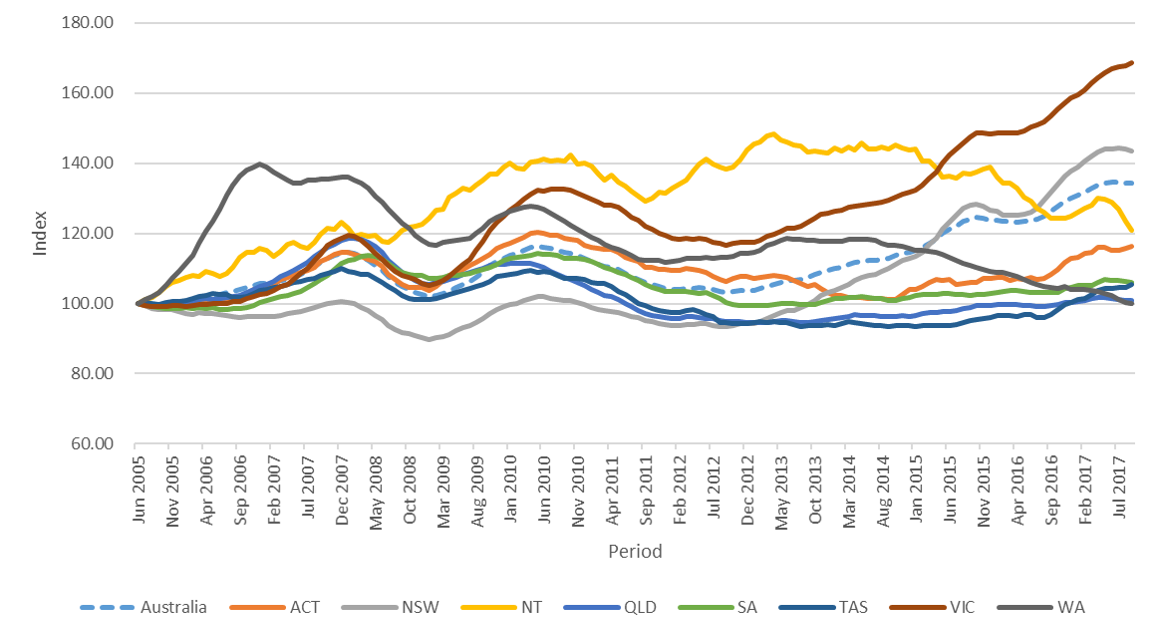
\includegraphics[width=\columnwidth]{Figures/Capital_houses_real_index_states.png}
 \caption{Real Capital Price Index (Houses) for Australia and by States}
 \label{fig:Capital_houses_real_index_states}
 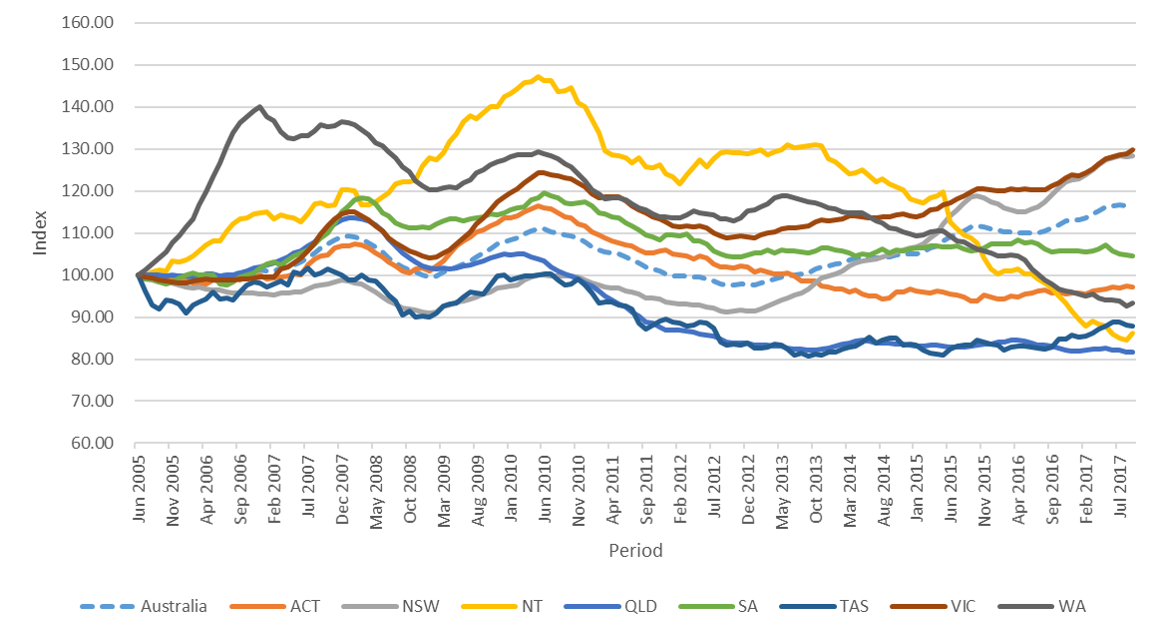
\includegraphics[width=\columnwidth]{Figures/Capital_units_real_index_states.png}
 \caption{Real Capital Price Index (Units) for Australia and by States}
 \label{fig:Capital_units_real_index_states}
\end{figure}


Figures \ref{fig:Capital_houses_real_index_states} and \ref{fig:Capital_units_real_index_states} show the real house price capital index from June 2005 to September 2017 for houses and units respectively. The house prices on average have increased by around 38\% since June 2005 with a CAGR of 2.47\%. The house prices in Victoria have seen the highest increase since 2005 of around 68\% with a CAGR of 4.32\%. New South Wales has a similar index movements but with lower price rise than Victoria of around 42\% with a CAGR of 2.9\%. The units have lower real price increases than houses on average. Units price index in Australia increased by around 18\% in September 2017 since June 2005 with CAGR of 1.35\%. The units price increase for Victoria and New South Wales was similar around 30\% with a CAGR of 2.1\%. The units price index for all other states closed at below 100 in September 2017 in real terms.




Figures \ref{fig:Rental_houses_real_index_states} and \ref{fig:Rental_units_real_index_states} show the real rental price index from June 2005 to September 2017 for houses and units respectively. For the period, the Australian real rental price index for houses on average has increased by around 12\% with a CAGR of 0.9\%. For New South Wales the house rental price index (real) has increased by 20\% with CAGR of 1.49\% while Victoria's house rental price index (real) has increased by 15\% with a CAGR of 1.14\%. The unit rental price index (real) for Australia has increase by 20\% with a CAGR of 1.49\% which is similar to that of Victoria. While for New South Wales, the units rental price index (real) has increased by 24\% with a CAGR of 1.77\%. The rental price index for Tasmania is available from October 2008 which is re-based to 100 and the rental price has remained constant as of September 2017.

In aggregate, we see that the real capital return for the period between June 2005 till September 2017 has been, on average, higher than the rental returns. When we look at it by property type, the real return on houses is higher than units in capital market whereas in the rental market there is higher returns on units than houses. This is in line with the expectations as lot of homeowners purchase units as part of investment and rent out the property whereas people who buy houses are mainly owner occupiers and therefore there is higher return on houses in capital markets.

\begin{figure}[!htb]
    \centering
     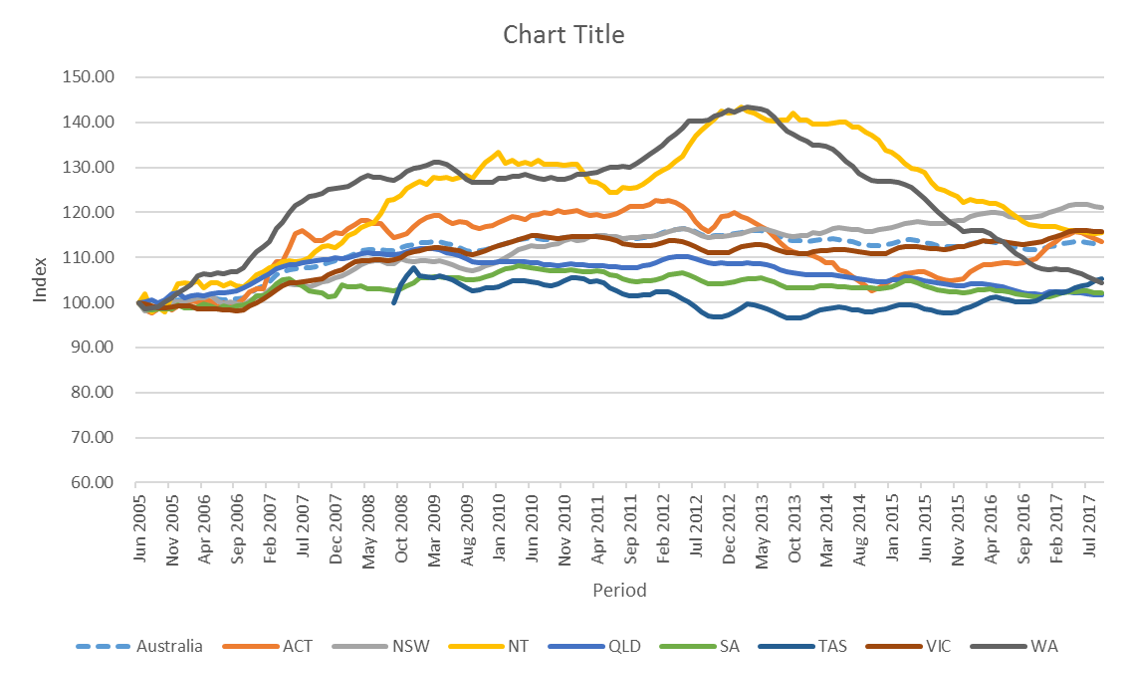
\includegraphics[width=\columnwidth]{Figures/Rental_houses_real_index_states.png}
 \caption{Real Rental Price Index (Houses) for Australia and by States}
 \label{fig:Rental_houses_real_index_states}
 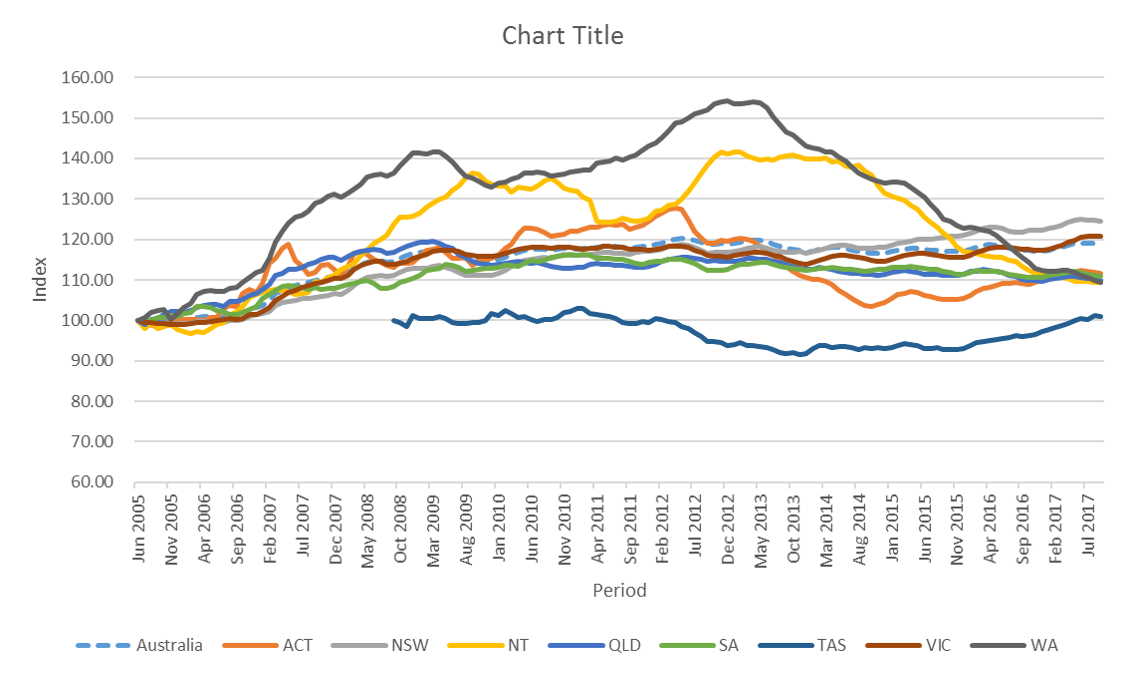
\includegraphics[width=\columnwidth]{Figures/Rental_units_real_index_states.png}
 \caption{Real Rental Price Index (Units) for Australia and by States}
 \label{fig:Rental_units_real_index_states}
\end{figure}


Tables \ref{tab:summary_stats_c_m} and \ref{tab:statistics_c_q} present the summary statistics for nationwide, states, greater capital cities and corresponding rest of states for the period June 2005 to September 2017 by property type for the real capital index returns at monthly and quarterly frequencies respectively. There are total of 148 monthly and 50 quarterly observations for all regions. The overall return at quarterly level is higher than the return at monthly level, as expected. In terms of property type, the real capital return for houses is higher than units with average return at national level for monthly (quarterly) frequency for houses being 0.4\% (1.2\%) and that for units being 0.3\% (0.9\%). The only region where units had higher average return is rest of South Australia where the average monthly (quarterly) return on houses is 0.1\% (0.2\%) and that for units is 0.2\% (0.6\%).

\newgeometry{margin=0.5in}
% Table generated by Excel2LaTeX from sheet 'capital index statistics'
\begin{table}[!ht]
  \centering
  \caption{Summary Statistics - Real Capital Monthly Log Returns (2005 - 2017)}  \label{tab:summary_stats_c_m}%
  \resizebox{0.65\textwidth}{!}{
 
\begin{threeparttable}
   
    \begin{tabular}{llHccHccHcc}
    \toprule
    \multicolumn{1}{l}{\multirow{2}[4]{*}{Region}} & \multicolumn{1}{l}{\multirow{2}[4]{*}{Sub Region}} & \multicolumn{3}{c}{All Dwellings} & \multicolumn{3}{c}{Houses} & \multicolumn{3}{c}{Units} \\
\cmidrule(lr){3-5} \cmidrule(lr){6-8}  \cmidrule(lr){9-11}           &       & \iffalse \multicolumn{1}{c}{Obs.} \fi & \multicolumn{1}{c}{Mean} & \multicolumn{1}{c}{Std. Dev.} & \iffalse \multicolumn{1}{c}{Obs.} \fi & \multicolumn{1}{c}{Mean} & \multicolumn{1}{c}{Std. Dev.} & \iffalse \multicolumn{1}{c}{Obs.} \fi & \multicolumn{1}{c}{Mean} & \multicolumn{1}{c}{Std. Dev.} \\
    
  &&& (\%)& (\%)&& (\%)& (\%)&& (\%)& (\%)\\
  
    \midrule
    
 
    Australia & Australia & 148   & 0.4 & 0.6 & 148   & 0.4 & 0.6 & 148   & 0.3 & 0.5 \\
    ACT   & ACT   & 148   & 0.3 & 0.6 & 148   & 0.3 & 0.7 & 148   & 0.2 & 0.7 \\
    \multirow{3}[0]{*}{NSW} & NSW   & 148   & 0.4 & 0.7 & 148   & 0.4 & 0.7 & 148   & 0.4 & 0.6 \\
          & GSYD  & 148   & 0.5 & 0.8 & 148   & 0.5 & 0.8 & 148   & 0.4 & 0.7 \\
          & RNSW  & 148   & 0.2 & 0.5 & 148   & 0.2 & 0.5 & 148   & 0.1 & 0.6 \\
    \multirow{3}[0]{*}{NT} & NT    & 148   & 0.3 & 1.0 & 148   & 0.3 & 1.1 & 148   & 0.1 & 1.3 \\
          & GDAR  & 148   & 0.2 & 1.0 & 148   & 0.3 & 1.2 & 148   & 0.1 & 1.4 \\
          & RNTE  & 148   & 0.3 & 1.7 & 148   & 0.4 & 2.0 & 148   & 0.2 & 2.6 \\
    \multirow{3}[0]{*}{QLD} & QLD   & 148   & 0.2 & 0.6 & 148   & 0.2 & 0.6 & 148   & 0.1 & 0.6 \\
          & GBRI  & 148   & 0.3 & 0.6 & 148   & 0.3 & 0.6 & 148   & 0.1 & 0.7 \\
          & RQLD  & 148   & 0.1 & 0.5 & 148   & 0.1 & 0.5 & 148   & 0.0 & 0.6 \\
    \multirow{3}[0]{*}{SA} & SA    & 148   & 0.2 & 0.5 & 148   & 0.2 & 0.5 & 148   & 0.2 & 0.7 \\
          & GADE  & 148   & 0.3 & 0.5 & 148   & 0.3 & 0.6 & 148   & 0.2 & 0.7 \\
          & RSAU  & 148   & 0.1 & 0.8 & 148   & 0.1 & 0.7 & 148   & 0.2 & 3.9 \\
    \multirow{3}[0]{*}{TAS} & TAS   & 148   & 0.2 & 0.6 & 148   & 0.2 & 0.6 & 148   & 0.1 & 1.2 \\
          & GHOB  & 148   & 0.3 & 0.7 & 148   & 0.3 & 0.7 & 148   & 0.1 & 1.5 \\
          & RTAS  & 148   & 0.2 & 0.6 & 148   & 0.2 & 0.7 & 148   & 0.1 & 1.8 \\
    \multirow{3}[0]{*}{VIC} & VIC   & 148   & 0.5 & 0.8 & 148   & 0.6 & 0.8 & 148   & 0.4 & 0.7 \\
          & GMEL  & 148   & 0.6 & 0.9 & 148   & 0.6 & 0.9 & 148   & 0.4 & 0.7 \\
          & RVIC  & 148   & 0.3 & 0.5 & 148   & 0.3 & 0.6 & 148   & 0.1 & 0.8 \\
    \multirow{3}[1]{*}{WA} & WA    & 148   & 0.2 & 1.0 & 148   & 0.2 & 1.0 & 148   & 0.2 & 1.0 \\
          & GPER  & 148   & 0.2 & 1.0 & 148   & 0.2 & 1.0 & 148   & 0.2 & 1.1 \\
          & RWAU  & 148   & 0.1 & 1.2 & 148   & 0.1 & 1.2 & 148   & -0.1 & 2.2 \\

    \bottomrule \\
   [-1.8ex]  
    
    \end{tabular}%

\begin{tablenotes}[para,flushleft]
  \LARGE
      Notes: This table reports the summary statistics of real capital index monthly log returns for nationwide, states, greater capital cities and corresponding rest of state for the period 2005 - 2017 with 148 observations for all regions.
\end{tablenotes}    

\end{threeparttable}


  }
  
   \caption{Summary Statistics - Real Capital Quarterly Log Returns (2005 - 2017)}
    \label{tab:statistics_c_q}%
   
   \resizebox{0.65\textwidth}{!}{
   
  \begin{threeparttable}
 
    \begin{tabular}{llHccHccHcc}
    \toprule
    \multicolumn{1}{l}{\multirow{2}[4]{*}{Region}} & \multicolumn{1}{l}{\multirow{2}[4]{*}{Sub Region}} & \multicolumn{3}{c}{All Dwellings} & \multicolumn{3}{c}{Houses} & \multicolumn{3}{c}{Units} \\
\cmidrule(lr){3-5} \cmidrule(lr){6-8}  \cmidrule(lr){9-11}           &       & \iffalse \multicolumn{1}{c}{Obs.} \fi & \multicolumn{1}{c}{Mean} & \multicolumn{1}{c}{Std. Dev.} & \iffalse \multicolumn{1}{c}{Obs.} \fi & \multicolumn{1}{c}{Mean} & \multicolumn{1}{c}{Std. Dev.} & \iffalse \multicolumn{1}{c}{Obs.} \fi & \multicolumn{1}{c}{Mean} & \multicolumn{1}{c}{Std. Dev.} \\
    
   
   &&& (\%)& (\%)&& (\%)& (\%)&& (\%)& (\%)\\

   
   
    \midrule
    
      Australia & Australia & 50    & 1.1 & 1.7 & 50    & 1.2 & 1.8 & 50    & 0.9 & 1.5 \\
    ACT   & ACT   & 50    & 0.8 & 1.6 & 50    & 0.9 & 1.7 & 50    & 0.6 & 1.6 \\
    \multirow{3}[0]{*}{NSW} & NSW   & 50    & 1.2 & 2.0 & 50    & 1.3 & 2.1 & 50    & 1.1 & 1.7 \\
          & GSYD  & 50    & 1.4 & 2.2 & 50    & 1.5 & 2.4 & 50    & 1.2 & 1.8 \\
          & RNSW  & 50    & 0.7 & 1.4 & 50    & 0.7 & 1.4 & 50    & 0.4 & 1.5 \\
    \multirow{3}[0]{*}{NT} & NT    & 50    & 0.8 & 2.3 & 50    & 1.0 & 2.5 & 50    & 0.3 & 2.9 \\
          & GDAR  & 50    & 0.7 & 2.5 & 50    & 1.0 & 2.7 & 50    & 0.3 & 3.1 \\
          & RNTE  & 50    & 0.9 & 3.2 & 50    & 1.0 & 3.7 & 50    & 0.5 & 4.1 \\
    \multirow{3}[0]{*}{QLD} & QLD   & 50    & 0.6 & 1.7 & 50    & 0.6 & 1.7 & 50    & 0.2 & 1.7 \\
          & GBRI  & 50    & 0.8 & 1.9 & 50    & 0.9 & 1.9 & 50    & 0.4 & 2.0 \\
          & RQLD  & 50    & 0.3 & 1.5 & 50    & 0.4 & 1.5 & 50    & 0.1 & 1.6 \\
    \multirow{3}[0]{*}{SA} & SA    & 50    & 0.7 & 1.4 & 50    & 0.7 & 1.4 & 50    & 0.7 & 1.7 \\
          & GADE  & 50    & 0.8 & 1.5 & 50    & 0.8 & 1.5 & 50    & 0.7 & 1.7 \\
          & RSAU  & 50    & 0.3 & 1.6 & 50    & 0.2 & 1.6 & 50    & 0.6 & 7.5 \\
    \multirow{3}[0]{*}{TAS} & TAS   & 50    & 0.7 & 1.5 & 50    & 0.7 & 1.5 & 50    & 0.4 & 2.5 \\
          & GHOB  & 50    & 0.8 & 1.8 & 50    & 0.9 & 1.8 & 50    & 0.3 & 3.1 \\
          & RTAS  & 50    & 0.6 & 1.4 & 50    & 0.6 & 1.5 & 50    & 0.4 & 3.0 \\
    \multirow{3}[0]{*}{VIC} & VIC   & 50    & 1.6 & 2.2 & 50    & 1.7 & 2.3 & 50    & 1.1 & 1.9 \\
          & GMEL  & 50    & 1.7 & 2.4 & 50    & 1.8 & 2.6 & 50    & 1.2 & 2.0 \\
          & RVIC  & 50    & 0.8 & 1.3 & 50    & 0.9 & 1.4 & 50    & 0.3 & 1.6 \\
    \multirow{3}[1]{*}{WA} & WA    & 50    & 0.6 & 2.8 & 50    & 0.7 & 2.8 & 50    & 0.5 & 2.9 \\
          & GPER  & 50    & 0.7 & 2.9 & 50    & 0.7 & 2.9 & 50    & 0.6 & 3.0 \\
          & RWAU  & 50    & 0.3 & 2.9 & 50    & 0.3 & 3.0 & 50    & -0.1 & 4.4 \\

  
  
    \bottomrule
    \end{tabular}%
 
\begin{tablenotes}[para,flushleft]
  \LARGE
      Notes: This table reports the summary statistics of real capital index quarterly log returns for nationwide, states, greater capital cities and corresponding rest of states for the period 2005 - 2017 with 50 observations for all regions.
\end{tablenotes}    

     
  \end{threeparttable} 
 
 
  }
  
  
  
\end{table}%

\restoregeometry


Tables \ref{tab:summary_stats_r_m} and \ref{tab:statistics_r_q} present the summary statistics for the period June 2005 to September 2017 by property type for the real rental index returns at monthly and quarterly frequencies respectively. For the period, there are 148 observations for all regions at monthly level except for Rest of Northern Territory houses and units that have 135 and 107 observations respectively, Rest of South Australia has 146 for Units, Tasmania and Greater Hobart have 109 and Rest of Tasmania has 108 observations. For quarterly frequency, there are 50 observations for all regions except for Rest of Northern Territory houses and units that have 45 and 36 observations respectively, Rest of South Australia with 49 for Units, Tasmania and Greater Hobart have 37 and Rest of Tasmania has 36 observations. The overall returns at quarterly level is higher than return at monthly level, as expected. In term of property type, the real rental return for houses at monthly level is the same as that of units at 0.3\%. However, at quarterly level, the return for units (0.8\%) is higher than that for houses (1\%).

\newgeometry{margin=0.5in}
% Table generated by Excel2LaTeX from sheet 'capital index statistics'
\begin{table}[!ht]
  \centering
  \caption{Summary Statistics - Real Rental Monthly Log Returns (2005 - 2017)}  \label{tab:summary_stats_r_m}%
  \resizebox{0.63\textwidth}{!}{
  \begin{threeparttable}
   
    \begin{tabular}{llHccHccHcc}
    \toprule
    \multicolumn{1}{l}{\multirow{2}[4]{*}{Region}} & \multicolumn{1}{l}{\multirow{2}[4]{*}{Sub Region}} & \multicolumn{3}{c}{All Dwellings} & \multicolumn{3}{c}{Houses} & \multicolumn{3}{c}{Units} \\
\cmidrule(lr){3-5} \cmidrule(lr){6-8}  \cmidrule(lr){9-11}           &       & \iffalse \multicolumn{1}{c}{Obs.} \fi & \multicolumn{1}{c}{Mean} & \multicolumn{1}{c}{Std. Dev.} & \iffalse \multicolumn{1}{c}{Obs.} \fi & \multicolumn{1}{c}{Mean} & \multicolumn{1}{c}{Std. Dev.} & \iffalse \multicolumn{1}{c}{Obs.} \fi & \multicolumn{1}{c}{Mean} & \multicolumn{1}{c}{Std. Dev.} \\
    

&&& (\%)& (\%)&& (\%)& (\%)&& (\%)& (\%)\\
    \midrule
    
    
 
      Australia & Australia & 148   & 0.3 & 0.3 & 148   & 0.3 & 0.3 & 148   & 0.3 & 0.3 \\
    ACT   & ACT   & 148   & 0.3 & 0.8 & 148   & 0.3 & 0.8 & 148   & 0.3 & 1.0 \\
    \multirow{3}[0]{*}{NSW} & NSW   & 148   & 0.3 & 0.4 & 148   & 0.3 & 0.4 & 148   & 0.4 & 0.4 \\
          & GSYD  & 148   & 0.4 & 0.4 & 148   & 0.4 & 0.4 & 148   & 0.4 & 0.4 \\
          & RNSW  & 148   & 0.3 & 0.6 & 148   & 0.2 & 0.7 & 148   & 0.3 & 0.5 \\
    \multirow{3}[0]{*}{NT} & NT    & 148   & 0.3 & 0.8 & 148   & 0.3 & 0.9 & 148   & 0.3 & 1.1 \\
          & GDAR  & 148   & 0.3 & 0.9 & 148   & 0.3 & 1.0 & 148   & 0.3 & 1.1 \\
          & RNTE  & 135   & 0.3 & 1.9 & 135   & 0.3 & 2.2 & 107   & 0.2 & 3.2 \\
    \multirow{3}[0]{*}{QLD} & QLD   & 148   & 0.2 & 0.4 & 148   & 0.2 & 0.4 & 148   & 0.3 & 0.5 \\
          & GBRI  & 148   & 0.3 & 0.3 & 148   & 0.3 & 0.3 & 148   & 0.3 & 0.5 \\
          & RQLD  & 148   & 0.2 & 0.6 & 148   & 0.1 & 0.6 & 148   & 0.2 & 0.6 \\
    \multirow{3}[0]{*}{SA} & SA    & 148   & 0.2 & 0.4 & 148   & 0.2 & 0.4 & 148   & 0.3 & 0.4 \\
          & GADE  & 148   & 0.2 & 0.3 & 148   & 0.2 & 0.4 & 148   & 0.3 & 0.4 \\
          & RSAU  & 148   & 0.1 & 1.7 & 148   & 0.1 & 1.8 & 146   & 0.1 & 2.9 \\
    \multirow{3}[0]{*}{TAS} & TAS   & 109   & 0.2 & 0.6 & 109   & 0.2 & 0.6 & 109   & 0.2 & 0.6 \\
          & GHOB  & 109   & 0.2 & 0.6 & 109   & 0.3 & 0.6 & 109   & 0.2 & 0.7 \\
          & RTAS  & 109   & 0.2 & 0.8 & 109   & 0.2 & 0.9 & 108   & 0.2 & 0.8 \\
    \multirow{3}[0]{*}{VIC} & VIC   & 148   & 0.3 & 0.3 & 148   & 0.3 & 0.3 & 148   & 0.3 & 0.4 \\
          & GMEL  & 148   & 0.3 & 0.3 & 148   & 0.3 & 0.3 & 148   & 0.3 & 0.4 \\
          & RVIC  & 148   & 0.2 & 0.6 & 148   & 0.2 & 0.6 & 148   & 0.2 & 1.1 \\
    \multirow{3}[1]{*}{WA} & WA    & 148   & 0.2 & 0.7 & 148   & 0.2 & 0.7 & 148   & 0.3 & 0.9 \\
          & GPER  & 148   & 0.3 & 0.8 & 148   & 0.3 & 0.7 & 148   & 0.3 & 0.9 \\
          & RWAU  & 148   & 0.1 & 1.2 & 148   & 0.1 & 1.3 & 148   & 0.2 & 3.8 \\

 
\bottomrule \\[-1.8ex] 

\end{tabular} 

\begin{tablenotes}[para,flushleft]
  \LARGE
       Notes: This table reports the summary statistics of real rental index monthly log returns for nationwide, states, greater capital cities and rest of states for the period 2005 - 2017. There are 148 obs. for all regions except for Rest of Northern Territory with 135 for Houses and 107 for Units, Rest of South Australia with 146 for Units, Tasmania and Greater Hobart with 109 and Rest of Tasmania with 108 observations.
\end{tablenotes}    



\end{threeparttable}

  }
  
   \caption{Summary Statistics - Real Rental Quarterly Log Returns (2005 - 2017)}
    \label{tab:statistics_r_q}%
   
   \resizebox{0.63\textwidth}{!}{
   
   \begin{threeparttable}
   
    \begin{tabular}{llHccHccHcc}
    \toprule
    \multicolumn{1}{l}{\multirow{2}[4]{*}{Region}} & \multicolumn{1}{l}{\multirow{2}[4]{*}{Sub Region}} & \multicolumn{3}{c}{All Dwellings} & \multicolumn{3}{c}{Houses} & \multicolumn{3}{c}{Units} \\
\cmidrule(lr){3-5} \cmidrule(lr){6-8}  \cmidrule(lr){9-11}           &       & \iffalse \multicolumn{1}{c}{Obs.} \fi & \multicolumn{1}{c}{Mean} & \multicolumn{1}{c}{Std. Dev.} & \iffalse \multicolumn{1}{c}{Obs.} \fi & \multicolumn{1}{c}{Mean} & \multicolumn{1}{c}{Std. Dev.} & \iffalse \multicolumn{1}{c}{Obs.} \fi & \multicolumn{1}{c}{Mean} & \multicolumn{1}{c}{Std. Dev.} \\
    

&&& (\%)& (\%)&& (\%)& (\%)&& (\%)& (\%)\\
    \midrule
    
    
      Australia & Australia & 50    & 0.8 & 1.0 & 50    & 0.8 & 1.1 & 50    & 1.0 & 0.9 \\
    ACT   & ACT   & 50    & 0.9 & 1.9 & 50    & 0.9 & 2.0 & 50    & 0.8 & 2.1 \\
    \multirow{3}[0]{*}{NSW} & NSW   & 50    & 1.0 & 1.0 & 50    & 0.9 & 1.3 & 50    & 1.1 & 0.9 \\
          & GSYD  & 50    & 1.0 & 1.0 & 50    & 0.9 & 1.3 & 50    & 1.1 & 1.0 \\
          & RNSW  & 50    & 0.6 & 1.5 & 50    & 0.6 & 1.6 & 50    & 1.0 & 1.0 \\
    \multirow{3}[0]{*}{NT} & NT    & 50    & -0.3 & 8.8 & 50    & -0.1 & 7.7 & 50    & -2.0 & 20.2 \\
          & GDAR  & 50    & -0.4 & 8.8 & 50    & -0.2 & 7.7 & 50    & -2.0 & 20.2 \\
          & RNTE  & 45    & 1.0 & 3.6 & 45    & 1.0 & 3.8 & 36    & 1.1 & 2.7 \\
    \multirow{3}[0]{*}{QLD} & QLD   & 50    & 0.7 & 0.9 & 50    & 0.6 & 0.8 & 50    & 0.6 & 1.7 \\
          & GBRI  & 50    & 0.8 & 0.9 & 50    & 0.8 & 0.9 & 50    & 0.7 & 1.8 \\
          & RQLD  & 50    & 0.6 & 1.0 & 50    & 0.5 & 1.0 & 50    & 0.7 & 1.1 \\
    \multirow{3}[0]{*}{SA} & SA    & 50    & 0.5 & 1.3 & 50    & 0.5 & 1.3 & 50    & 0.8 & 0.9 \\
          & GADE  & 50    & 0.8 & 0.9 & 50    & 0.7 & 0.9 & 50    & 0.9 & 0.9 \\
          & RSAU  & 50    & 0.2 & 2.1 & 50    & 0.2 & 2.3 & 49    & 0.3 & 5.5 \\
    \multirow{3}[0]{*}{TAS} & TAS   & 37    & 0.6 & 1.5 & 37    & 0.7 & 1.7 & 37    & 0.5 & 1.1 \\
          & GHOB  & 37    & 0.7 & 1.5 & 37    & 0.8 & 1.6 & 37    & 0.6 & 1.4 \\
          & RTAS  & 37    & 0.5 & 2.0 & 37    & 0.5 & 2.2 & 36    & 0.4 & 1.1 \\
    \multirow{3}[0]{*}{VIC} & VIC   & 50    & 0.9 & 0.9 & 50    & 0.9 & 0.9 & 50    & 1.0 & 1.0 \\
          & GMEL  & 50    & 1.0 & 1.0 & 50    & 1.0 & 1.0 & 50    & 1.0 & 1.1 \\
          & RVIC  & 50    & 0.5 & 1.4 & 50    & 0.5 & 1.4 & 50    & 0.5 & 1.8 \\
    \multirow{3}[1]{*}{WA} & WA    & 50    & 0.7 & 2.1 & 50    & 0.7 & 2.1 & 50    & 0.8 & 2.4 \\
          & GPER  & 50    & 0.8 & 2.2 & 50    & 0.8 & 2.1 & 50    & 0.8 & 2.4 \\
          & RWAU  & 50    & 0.4 & 2.6 & 50    & 0.4 & 2.7 & 50    & 0.6 & 7.8 \\

 
  
\bottomrule \\[-1.8ex] 

\end{tabular} 

\begin{tablenotes}[para,flushleft]
  \LARGE
        Notes: This table reports the summary statistics for real rental index quarterly log returns for nationwide, states, greater capital cities and rest of states for the period 2005 - 2017. There are 50 observations for all regions except for Rest of Northern Territory with 45 for Houses and 36 for Units, Rest of South Australia with 49 for Units, Tasmania and Greater Hobart with 37 and Rest of Tasmania with 36 observations.
\end{tablenotes}    



\end{threeparttable}
  }
  
  
  
\end{table}%

\restoregeometry


\section{Results}

\subsection{Summary Results across all Regions}


Tables \ref{tab:count_m_c} and \ref{tab:count_q_c} report the percentage distribution of regions with persistence in real housing capital monthly and quarterly returns from the period 2005 to 2017. At nationwide, state and GCC level, all regions have persistent returns at 1\% and 5\% significance levels for all dwellings. At SA4 (88 regions) and SA3 (332 regions) geographic region levels, we find that 83\% (84\%) and 69\% (75\%) of the regions are persistent at 1\% (5\%) significance. Across property types, overall there is higher persistence in houses than in units in capital returns.

The results are also consistent when we test the results using Runs two-sided test. We also test the persistence using one-sided runs tests (Runs (-) and Runs (+)). The runs (-) and runs (+) tests for the null of random walk against the alternative of trend and first order serial correlations respectively. We find that in the former, we reject the null of random walk in the favour of trend and in the case of latter, we do not find evidence of first order serial correlation. There is less persistence found in the quarterly level data however the patterns of persistence in variance ratio and runs test and across property types are similar.


Tables \ref{tab:count_m_r} and \ref{tab:count_q_r} report the percentage distribution of regions with persistence in real housing rental monthly and quarterly returns from the period 2005 to 2017. We find that overall for all dwellings there are less regions with persistent returns in rental market relative to capital market. The returns at nationwide level are found to be persistence. Out of eight states, we find 88\% and 100\% have persistent returns at 1\% and 5\% significance levels. For GCC region level, we find 60\% and 73\% of 15 regions to have persistent returns. At SA4 and SA3 level, we find 57\% (66\%) and 42\% (50\%) regions have persistent returns at 1\% (5\%) significant levels. If we look across property types in rental market, we find that units have greater number of regions with persistence as compared to houses vis-a-vis capital markets. 

In runs test two-sided, we find the result are similar. In case of runs (-) and runs (+), we find significant results in the favour of trend and no negative first order serial correlation respectively. Again for quarterly level data, there are lesser regions with persistence than at monthly data, however there are similar patterns in the persistence results for both variance ratio and runs test across property types.

Overall, as we go from lower to higher level of geographic regions, we find that there is more proportion of regions that have persistent returns indicating a stronger persistence in returns of regions that have persistence.

%%%%%%%%%%%%%%%%%%%%%%%%%%%%

\newgeometry{margin=1in}
% Table generated by Excel2LaTeX from sheet 'Sheet3'
\begin{table}[!ht]
  \centering
  
  \caption{\% Distribution of Regions with Persistence in Housing Capital (Monthly) Returns (2005---2017)}  \label{tab:count_m_c}%
  
    \resizebox{\textwidth}{!}{
   
   
   
    \begin{tabu} to \textwidth {X[0.65,l]X[0.9,l]X[1,c]X[0.8,r]X[0.8,r]X[0.8,r]X[0.8,r]X[0.8,r]X[0.8,r]X[0.8,r]X[0.8,r]}
    \toprule
    Type & 
    Level & 
    No. of Regions &
    VR Signif. 1\% &
    VR Signif. 5\% &
    Runs Signif 1\% &
    Runs Signif 5\% &
    Runs (-) Signif. 1\% &
    Runs (-) Signif. 5\% &
    Runs (+) Signif. 1\% &
    Runs (+) Signif. 5\%\\
    \midrule
 
  %  Dwelling & Nation & 1     & 1     & 1     & 1     & 1     & 1     & 1     & 0     & 0 \\
  %        & State & 8     & 8     & 8     & 8     & 8     & 8  %   & 8     & 0     & 0 \\
  %        & GCC   & 15    & 15    & 15    & 14    & 15    & 14 %   & 15    & 0     & 0 \\
  %        & SA4   & 88    & 73    & 74    & 68    & 72    & 70 %   & 74    & 0     & 1 \\
  %        & SA3   & 334   & 229   & 249   & 176   & 217   & 190   & 228   & 0     & 4 \\
  %  Houses & Nation & 1     & 1     & 1     & 1     & 1     & 1     & 1     & 0     & 0 \\
  %        & State & 8     & 8     & 8     & 7     & 7     & 7     & 7     & 0     & 0 \\
  %        & GCC   & 15    & 15    & 15    & 14    & 15    & 15    & 15    & 0     & 0 \\
  %        & SA4   & 88    & 73    & 74    & 68    & 73    & 70    & 75    & 0     & 1 \\
  %        & SA3   & 334   & 223   & 239   & 163   & 193   & 176   & 215   & 0     & 3 \\
  %  Units & Nation & 1     & 1     & 1     & 1     & 1     & 1     & 1     & 0     & 0 \\
   %       & State & 8     & 7     & 8     & 6     & 7     & 6     & 7     & 0     & 0 \\
    %      & GCC   & 15    & 10    & 12    & 7     & 9     & 8     & 11    & 0     & 0 \\
     %     & SA4   & 88    & 47    & 52    & 34    & 44    & 39    & 48    & 0     & 2 \\
      %    & SA3   & 331   & 140   & 169   & 82    & 120   & 97    & 138   & 1     & 5 \\
      
          
         \multicolumn{1}{l}{Dwellings} & Nation & 1     & 100 & 100 & 100 & 100 & 100 & 100 & 0   & 0 \\
          & State & 8     & 100 & 100 & 100 & 100 & 100 & 100 & 0   & 0 \\
          & GCC   & 15    & 100 & 100 & 93  & 100 & 93  & 100 & 0   & 0 \\
          & SA4   & 88    & 83  & 84  & 77  & 82  & 80  & 84  & 0   & 1 \\
          & SA3   & 334   & 69  & 75  & 53  & 65  & 57  & 68  & 0   & 1 \\
    \multicolumn{1}{l}{Houses} & Nation & 1     & 100 & 100 & 100 & 100 & 100 & 100 & 0   & 0 \\
          & State & 8     & 100 & 100 & 88  & 88  & 88  & 88  & 0   & 0 \\
          & GCC   & 15    & 100 & 100 & 93  & 100 & 100 & 100 & 0   & 0 \\
          & SA4   & 88    & 83  & 84  & 77  & 83  & 80  & 85  & 0   & 1 \\
          & SA3   & 334   & 67  & 72  & 49  & 58  & 53  & 64  & 0   & 1 \\
    \multicolumn{1}{l}{Units} & Nation & 1     & 100 & 100 & 100 & 100 & 100 & 100 & 0   & 0 \\
          & State & 8     & 88  & 100 & 75  & 88  & 75  & 88  & 0   & 0 \\
          & GCC   & 15    & 67  & 80  & 47  & 60  & 53  & 73  & 0   & 0 \\
          & SA4   & 88    & 53  & 59  & 39  & 50  & 44  & 55  & 0   & 2 \\
          & SA3   & 331   & 42  & 51  & 25  & 36  & 29  & 42  & 0   & 2 \\

         \bottomrule
    \end{tabu}%
    }
   \bigskip
    
    
     \caption{\% Distribution of Regions with Persistence in Housing Capital (Quarterly) Returns (2005---2017)} \label{tab:count_q_c}
\resizebox{\textwidth}{!}{


\begin{tabu} to \textwidth {X[0.65,l]X[0.9,l]X[1,c]X[0.8,r]X[0.8,r]X[0.8,r]X[0.8,r]X[0.8,r]X[0.8,r]X[0.8,r]X[0.8,r]}
    \toprule
    Type & 
    Level & 
    No. of Regions & 
    VR Signif. 1\% & 
    VR Signif. 5\% & 
    Runs Signif 1\% &
    Runs Signif 5\% &
    Runs (-) Signif. 1\% & 
    Runs (-) Signif. 5\% & 
    Runs (+) Signif. 1\% & 
    Runs (+) Signif. 5\% \\
    \midrule
    
 

 %   Dwelling & Nation & 1     & 1     & 1     & 1     & 1     & 1     & 1     & 0     & 0 \\
 %         & State & 8     & 4     & 7     & 7     & 8     & 8     & 8     & 0     & 0 \\
 %         & GCC   & 15    & 8     & 11    & 8     & 11    & 11    & 13    & 0     & 0 \\
 %         & SA4   & 88    & 49    & 62    & 50    & 63    & 56    & 65    & 1     & 2 \\
 %         & SA3   & 334   & 159   & 206   & 126   & 165   & 136   & 186   & 0     & 3 \\
 %   Houses & Nation & 1     & 1     & 1     & 1     & 1     & 1     & 1     & 0     & 0 \\
  %        & State & 8     & 3     & 7     & 6     & 8     & 7     & 8     & 0     & 0 \\
  %        & GCC   & 15    & 6     & 12    & 9     & 10    & 10    & 11    & 0     & 0 \\
   %       & SA4   & 88    & 48    & 65    & 47    & 59    & 52    & 61    & 0     & 1 \\
%          & SA3   & 334   & 146   & 199   & 109   & 157   & 125   & 174   & 1     & 1 \\
 %   Units & Nation & 1     & 0     & 0     & 1     & 1     & 1     & 1     & 0     & 0 \\
  %        & State & 8     & 4     & 6     & 5     & 5     & 5     & 6     & 0     & 0 \\
   %       & GCC   & 15    & 5     & 8     & 7     & 8     & 8     & 9     & 0     & 0 \\
   %       & SA4   & 88    & 30    & 45    & 22    & 33    & 23    & 41    & 0     & 1 \\
    %      & SA3   & 331   & 70    & 130   & 46    & 84    & 63    & 104   & 0     & 7 \\
   
 
 
     \multicolumn{1}{l}{Dwellings} & Nation & 1     &                     100  &                     100  &                        100  &                        100  &                              100  &                              100  &                                  0    &                                  0    \\
          & State & 8     &                       50  &                       88  &                           88  &                        100  &                              100  &                              100  &                                  0    &                                  0    \\
          & GCC   & 15    &                       53  &                       73  &                           53  &                           73  &                                73  &                                87  &                                  0    &                                  0    \\
          & SA4   & 88    &                       56  &                       70  &                           57  &                           72  &                                64  &                                74  &                                   1  &                                   2  \\
          & SA3   & 334   &                       48  &                       62  &                           38  &                           49  &                                41  &                                56  &                                  0    &                                   1  \\
    \multicolumn{1}{l}{Houses} & Nation & 1     &                     100  &                     100  &                        100  &                        100  &                              100  &                              100  &                                  0    &                                  0    \\
          & State & 8     &                       38  &                       88  &                           75  &                        100  &                                88  &                              100  &                                  0    &                                  0    \\
          & GCC   & 15    &                       40  &                       80  &                           60  &                           67  &                                67  &                                73  &                                  0    &                                  0    \\
          & SA4   & 88    &                       55  &                       74  &                           53  &                           67  &                                59  &                                69  &                                  0    &                                   1  \\
          & SA3   & 334   &                       44  &                       60  &                           33  &                           47  &                                37  &                                52  &                                   0  &                                   0  \\
    \multicolumn{1}{l}{Units} & Nation & 1     &                        0    &                        0    &                        100  &                        100  &                              100  &                              100  &                                  0    &                                  0    \\
          & State & 8     &                       50  &                       75  &                           63  &                           63  &                                63  &                                75  &                                  0    &                                  0    \\
          & GCC   & 15    &                       33  &                       53  &                           47  &                           53  &                                53  &                                60  &                                  0    &                                  0    \\
          & SA4   & 88    &                       34  &                       51  &                           25  &                           38  &                                26  &                                47  &                                  0    &                                   1  \\
          & SA3   & 331   &                       21  &                       39  &                           14  &                           25  &                                19  &                                31  &                                  0    &                                   2  \\

 
 
 
    \bottomrule
    \end{tabu}%
 }
  
\end{table}%

%% Table generated by Excel2LaTeX from sheet 'Sheet3'
\begin{table}[!htb]
  \centering
  \caption{Distribution of Regions with Persistent Housing Capital Quarterly Returns (2005 - 2017)}
    \resizebox{0.95\textwidth}{!}{
    \begin{tabu} to \textwidth {X[0.8,l]X[0.5,l]X[0.75,c]X[0.6,c]X[0.6,c]X[0.6,c]X[0.6,c]X[0.6,c]X[0.6,c]}
    \toprule
    Type & 
    Region & 
    No. of Regions & 
    VR Signif. 1\% & 
    VR Signif. 5\% & 
    Runs (-) Signif. 1\% & 
    Runs (-) Signif. 5\% & 
    Runs (+) Signif. 1\% & 
    Runs (+) Signif. 5\% \\
    \midrule
    
 
    \multicolumn{1}{l}{All Dwellings} & Country & 1     & 1     & 1     & 1     & 1     & 0     & 0 \\
          & State & 8     & 4     & 7     & 8     & 8     & 0     & 0 \\
          & GCC   & 15    & 8     & 11    & 11    & 13    & 0     & 0 \\
          & SA4   & 88    & 49    & 62    & 56    & 65    & 1     & 2 \\
          & SA3   & 334   & 159   & 206   & 136   & 186   & 0     & 3 \\
    \multicolumn{1}{l}{Houses} & Country & 1     & 1     & 1     & 1     & 1     & 0     & 0 \\
          & State & 8     & 4     & 7     & 8     & 8     & 0     & 0 \\
          & GCC   & 15    & 8     & 11    & 11    & 13    & 0     & 0 \\
          & SA4   & 88    & 49    & 62    & 56    & 65    & 1     & 2 \\
          & SA3   & 334   & 159   & 206   & 136   & 186   & 0     & 3 \\
    \multicolumn{1}{l}{Units} & Country & 1     & 1     & 1     & 1     & 1     & 0     & 0 \\
          & State & 8     & 4     & 7     & 8     & 8     & 0     & 0 \\
          & GCC   & 15    & 8     & 11    & 11    & 13    & 0     & 0 \\
          & SA4   & 88    & 49    & 62    & 56    & 65    & 1     & 2 \\
          & SA3   & 334   & 159   & 206   & 136   & 186   & 0     & 3 \\
   

    
  
    \bottomrule
    \end{tabu}%
  \label{tab:count_q_c}%
  }
\end{table}%

\restoregeometry


\newgeometry{margin=1in}
% Table generated by Excel2LaTeX from sheet 'Sheet3'
\begin{table}[!ht]
  \centering
  
  \caption{\% Distribution of Regions with Persistence in Housing Rental (Monthly) Returns (2005---2017)}  \label{tab:count_m_r}%
  
    \resizebox{\textwidth}{!}{
   
   
   
  \begin{tabu} to \textwidth {X[0.65,l]X[0.9,l]X[1,c]X[0.8,r]X[0.8,r]X[0.8,r]X[0.8,r]X[0.8,r]X[0.8,r]X[0.8,r]X[0.8,r]}
    \toprule
    Type & 
    Level & 
    No. of Regions &
    VR Signif. 1\% &
    VR Signif. 5\% &
    Runs Signif 1\% &
    Runs Signif 5\% &
    Runs (-) Signif. 1\% &
    Runs (-) Signif. 5\% &
    Runs (+) Signif. 1\% &
    Runs (+) Signif. 5\%\\
    \midrule
  

%     Dwellings & Nation & 1     & 1     & 0     & 1     & 0     & 1     & 0     & 0     & 0 \\
 %         & State & 8     & 7     & 1     & 8     & 0     & 8     & 0     & 0     & 0 \\
  %        & GCC   & 15    & 9     & 2     & 12    & 0     & 12    & 0     & 0     & 0 \\
  %        & SA4   & 88    & 50    & 8     & 52    & 14    & 58    & 9     & 0     & 0 \\
  %        & SA3   & 332   & 141   & 25    & 110   & 53    & 133   & 61    & 0     & 2 \\
  %  Houses & Nation & 1     & 1     & 0     & 1     & 0     & 1     & 0     & 0     & 0 \\
    %      & State & 8     & 7     & 0     & 8     & 0     & 8     & 0     & 0     & 0 \\
    %      & GCC   & 15    & 10    & 1     & 11    & 1     & 12    & 0     & 0     & 0 \\
    %      & SA4   & 88    & 36    & 3     & 41    & 8     & 44    & 9     & 0     & 1 \\
    %      & SA3   & 332   & 87    & 30    & 89    & 54    & 106   & 56    & 0     & 4 \\
%    Units & Nation & 1     & 1     & 0     & 1     & 0     & 1     & 0     & 0     & 0 \\
 %         & State & 8     & 8     & 0     & 8     & 0     & 8     & 0     & 0     & 0 \\
  %        & GCC   & 15    & 10    & 1     & 12    & 0     & 12    & 0     & 0     & 0 \\
  %        & SA4   & 88    & 53    & 5     & 56    & 6     & 61    & 9     & 0     & 1 \\
   %       & SA3   & 333   & 173   & 21    & 140   & 42    & 153   & 62    & 0     & 3 \\
  

       \multicolumn{1}{l}{Dwellings} & Nation & 1     & 100   & 100   & 100   & 100   & 100   & 100   & 0     & 0  \\
          & State & 8     & 88    & 100   & 100   & 100   & 100   & 100   & 0     & 0  \\
          & GCC   & 15    & 60    & 73    & 80    & 80    & 80    & 80    & 0     & 0  \\
          & SA4   & 88    & 57    & 66    & 59    & 75    & 66    & 76    & 0     & 0  \\
          & SA3   & 332   & 42    & 50    & 33    & 49    & 40    & 58    & 0     & 1  \\
    \multicolumn{1}{l}{Houses} & Nation & 1     & 100   & 100   & 100   & 100   & 100   & 100   & 0     & 0  \\
          & State & 8     & 88    & 88    & 100   & 100   & 100   & 100   & 0     & 0  \\
          & GCC   & 15    & 67    & 73    & 73    & 80    & 80    & 80    & 0     & 0  \\
          & SA4   & 88    & 41    & 44    & 47    & 56    & 50    & 60    & 0     & 1  \\
          & SA3   & 332   & 26    & 35    & 27    & 43    & 32    & 49    & 0     & 1  \\
    \multicolumn{1}{l}{Units} & Nation & 1     & 100   & 100   & 100   & 100   & 100   & 100   & 0     & 0  \\
          & State & 8     & 100   & 100   & 100   & 100   & 100   & 100   & 0     & 0  \\
          & GCC   & 15    & 67    & 73    & 80    & 80    & 80    & 80    & 0     & 0  \\
          & SA4   & 88    & 60    & 66    & 64    & 70    & 69    & 80    & 0     & 1  \\
          & SA3   & 333   & 52    & 58    & 42    & 55    & 46    & 65    & 0     & 1  \\

    
  
         \bottomrule
    \end{tabu}%
    }
   \bigskip
    
    
     \caption{\% Distribution of Regions with Persistence in Housing Rental (Quarterly) Returns (2005---2017)}  \label{tab:count_q_r}
     
\resizebox{\textwidth}{!}{


\begin{tabu} to \textwidth {X[0.65,l]X[0.9,l]X[1,c]X[0.8,r]X[0.8,r]X[0.8,r]X[0.8,r]X[0.8,r]X[0.8,r]X[0.8,r]X[0.8,r]}
    \toprule
    Type & 
    Level & 
    No. of Regions & 
    VR Signif. 1\% & 
    VR Signif. 5\% & 
    Runs Signif 1\% &
    Runs Signif 5\% &
    Runs (-) Signif. 1\% & 
    Runs (-) Signif. 5\% & 
    Runs (+) Signif. 1\% & 
    Runs (+) Signif. 5\% \\
    \midrule
 
    
 %   Dwellings & Nation & 1     & 0     & 0     & 0     & 0     & 0     & 0     & 0     & 0 \\
 %         & State & 8     & 3     & 1     & 1     & 1     & 2     & 0     & 0     & 0 \\
  %        & GCC   & 15    & 4     & 1     & 2     & 1     & 3     & 0     & 0     & 0 \\
  %        & SA4   & 88    & 23    & 4     & 8     & 7     & 13    & 5     & 0     & 0 \\
  %        & SA3   & 332   & 52    & 29    & 22    & 23    & 29    & 33    & 1     & 6 \\
  %  Houses & Nation & 1     & 1     & 0     & 0     & 0     & 0     & 0     & 0     & 0 \\
  %        & State & 8     & 5     & 0     & 2     & 0     & 2     & 1     & 0     & 0 \\
  %      & GCC   & 15    & 5     & 1     & 2     & 2     & 3     & 3     & 0     & 0 \\
  %        & SA4   & 88    & 20    & 7     & 8     & 4     & 9     & 10    & 0     & 0 \\
  %        & SA3   & 332   & 34    & 18    & 17    & 25    & 23    & 35    & 0     & 3 \\
  % Units & Nation & 1     & 0     & 1     & 0     & 0     & 0     & 0     & 0     & 0 \\
  %        & State & 8     & 4     & 1     & 2     & 0     & 2     & 0     & 0     & 0 \\
  %        & GCC   & 15    & 5     & 1     & 4     & 0     & 4     & 0     & 0     & 0 \\
  %        & SA4   & 88    & 24    & 5     & 9     & 8     & 13    & 9     & 0     & 0 \\
  %        & SA3   & 333   & 71    & 24    & 28    & 21    & 34    & 31    & 1     & 6 \\
  
  
     \multicolumn{1}{l}{Dwellings} & Nation & 1     & 0     & 0     & 0     & 0     & 0     & 0     & 0     & 0  \\
          & State & 8     & 38    & 50    & 13    & 25    & 25    & 25    & 0     & 0  \\
          & GCC   & 15    & 27    & 33    & 13    & 20    & 20    & 20    & 0     & 0  \\
          & SA4   & 88    & 26    & 31    & 9     & 17    & 15    & 20    & 0     & 0  \\
          & SA3   & 332   & 16    & 24    & 7     & 14    & 9     & 19    & 0     & 2  \\
    \multicolumn{1}{l}{Houses} & Nation & 1     & 100   & 100   & 0     & 0     & 0     & 0     & 0     & 0  \\
          & State & 8     & 63    & 63    & 25    & 25    & 25    & 38    & 0     & 0  \\
          & GCC   & 15    & 33    & 40    & 13    & 27    & 20    & 40    & 0     & 0  \\
          & SA4   & 88    & 23    & 31    & 9     & 14    & 10    & 22    & 0     & 0  \\
          & SA3   & 332   & 10    & 16    & 5     & 13    & 7     & 17    & 0     & 1  \\
    \multicolumn{1}{l}{Units} & Nation & 1     & 0     & 100   & 0     & 0     & 0     & 0     & 0     & 0  \\
          & State & 8     & 50    & 63    & 25    & 25    & 25    & 25    & 0     & 0  \\
          & GCC   & 15    & 33    & 40    & 27    & 27    & 27    & 27    & 0     & 0  \\
          & SA4   & 88    & 27    & 33    & 10    & 19    & 15    & 25    & 0     & 0  \\
          & SA3   & 333   & 21    & 29    & 8     & 15    & 10    & 20    & 0     & 2  \\

  
 
    \bottomrule
    \end{tabu}%
 }
  
\end{table}%

\restoregeometry

%%%%%%%%%%%%%%%%%%%%%%%%%%%%



\begin{sidewaysfigure}[!htbp]
    \centering
     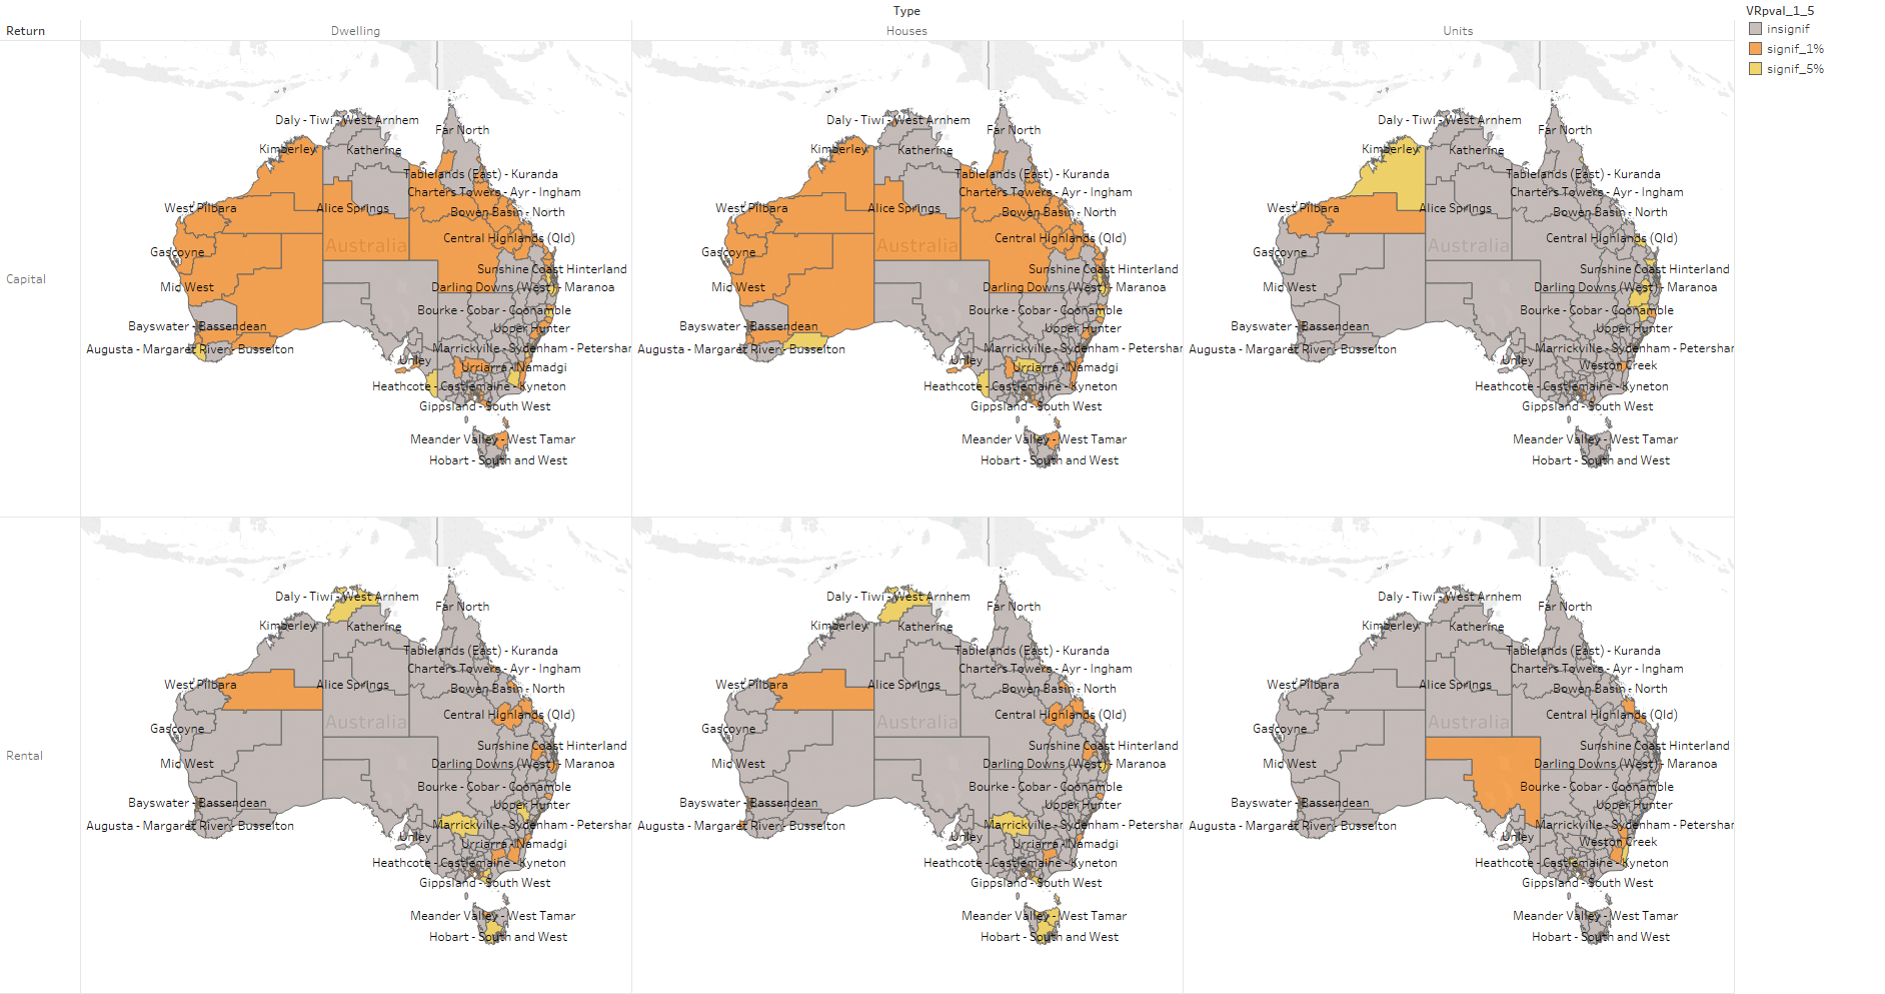
\includegraphics[width=\columnwidth]{Figures/maps_monthly_all.png}
 \caption{Persistence at SA3 geographic level by property type - Capital and Rental Monthly Returns}
 \label{fig:maps_monthly_all}
\end{sidewaysfigure}


\begin{sidewaysfigure}[!htbp]
    \centering
     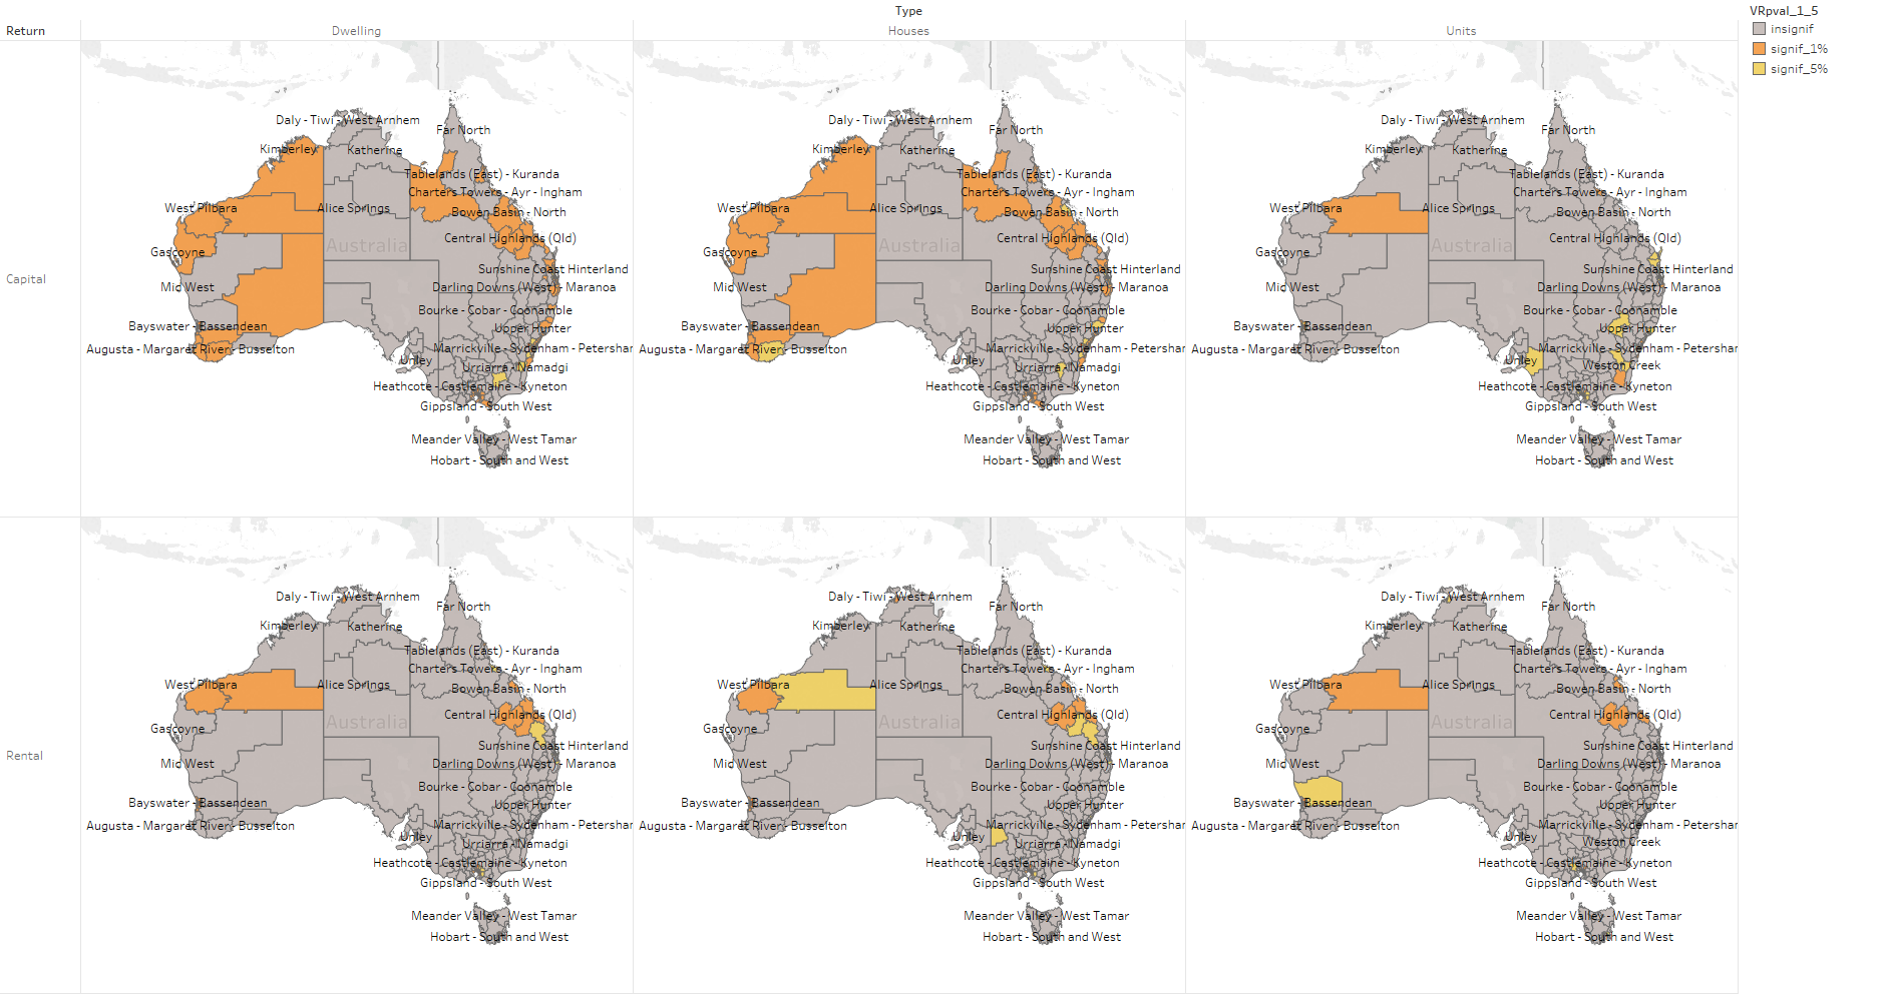
\includegraphics[width=\columnwidth]{Figures/maps_quarterly_all.png}
 \caption{Persistence at SA3 geographic level by property type - Capital and Rental Monthly Returns}
 \label{fig:maps_quarterly_all}
\end{sidewaysfigure}



\subsection{Results - Wild Bootstrap Automatic Variance Ratio Test}


Tables \ref{tab:results_m} and \ref{tab:results_q_c} present the wild bootstrap automatic variance ratio test results for real monthly and quarterly capital returns respectively at nationwide, state, greater capital cities and rest of states levels. Panels A, B and C provide results for all dwelling, houses and units respectively. The tables report the automatic variance ratio (VRSum), test statistics and the p-value which is calculated from the boostrapped sample distribution of the variance ratios and represents the proportion of cases in which the VRSum (t-statistic) lies between the 95\% confidence interval. The CI.VRSum.lower and CI.VRSum.upper, and CI.stat.lower and CI.stat.upper represent the 2.5 percentile and 97.5 percentile of the bootstrapped distribution.

We find that for all dwellings and houses, all regions have persistent returns at 1\% significance levels. For units, overall, we have less persistence than for houses. Nationwide the capital returns are persistent at 1\% level. At state level, all states have persistent returns at 1\% level except with Tasmania where the return are persistent at 5\% significance. Among greater cities, Greater Hobart is persistent at 5\% significance and for rest for states, we find that for \textit{Rest of Northern Territory}, \textit{Rest of South Australia} and \textit{Rest of Tasmania}, we cannot the reject the null of random walk at 5\% level. \textit{Rest of Western Australia} is found to have persistent capital returns at 5\% significance. 

At quarterly level, there are lesser number of regions with persistent returns but the pattern of persistence across property types is similar.


\newgeometry{margin=1in}
% Table generated by Excel2LaTeX from sheet 'Sheet5'
\begin{table}[htbp]
  \centering
  \caption{Capital Return - Wild Bootstrap Automatic Variance Ratio Test Result (Monthly)}
    \label{tab:results_m}%

     \resizebox{0.8\textwidth}{!}{
    \begin{tabular}{llrrrrrrr}
    \multicolumn{9}{c}{Panel A - All Dwellings} \\
    \midrule
    Region & Sub Region & \multicolumn{1}{l}{ VRsum} & \multicolumn{1}{l}{ test.stat} & \multicolumn{1}{l}{ pval} & \multicolumn{1}{l}{ CI.VRsum.lower} & \multicolumn{1}{l}{ CI.VRsum.upper} & \multicolumn{1}{l}{ CI.stat.lower} & \multicolumn{1}{l}{ CI.stat.upper} \\
    \midrule
    
  
    Australia & Australia & 6.9316 & 8.8230 & 0     & 0.6835 & 1.5810 & -1.8472 & 2.7688 \\
    ACT   & ACT   & 5.4752 & 12.5949 & 0     & 0.7350 & 1.4862 & -1.5490 & 2.2893 \\
    \multirow{3}[0]{*}{NSW} & NSW   & 10.8795 & 16.0241 & 0     & 0.6575 & 1.4918 & -1.9910 & 2.4128 \\
          & GSYD  & 10.5431 & 15.7791 & 0     & 0.6514 & 1.5145 & -1.9848 & 2.4041 \\
          & RNSW  & 8.7782 & 16.5977 & 0     & 0.6735 & 1.4553 & -1.8852 & 2.2190 \\
    \multirow{3}[0]{*}{NT} & NT    & 3.1648 & 7.8435 & 0     & 0.7767 & 1.2816 & -1.3389 & 1.4675 \\
          & GDAR  & 2.7761 & 6.6982 & 0     & 0.7573 & 1.2875 & -1.4452 & 1.5106 \\
          & RNT   & 1.3574 & 1.8292 & 0     & 0.8479 & 1.1703 & -0.9575 & 0.9549 \\
    \multirow{3}[0]{*}{QLD} & QLD   & 7.7572 & 10.2220 & 0     & 0.5923 & 1.7033 & -2.2978 & 3.1541 \\
          & GBRI  & 7.8993 & 10.1888 & 0     & 0.5952 & 1.6806 & -2.2828 & 3.1054 \\
          & RQLD  & 6.8993 & 11.0072 & 0     & 0.6152 & 1.7200 & -2.1885 & 3.3510 \\
    \multirow{3}[0]{*}{SA} & SA    & 6.4146 & 12.2984 & 0     & 0.6423 & 1.6283 & -2.0580 & 2.6855 \\
          & GADE  & 6.9592 & 13.1219 & 0     & 0.6285 & 1.6795 & -2.1040 & 2.9718 \\
          & RSAU  & 1.9703 & 4.0661 & 0     & 0.7934 & 1.3310 & -1.2250 & 1.6827 \\
    \multirow{3}[0]{*}{TAS} & TAS   & 5.2528 & 11.6764 & 0     & 0.6823 & 1.5421 & -1.8626 & 2.5038 \\
          & GHOB  & 4.1083 & 10.1835 & 0     & 0.7289 & 1.3821 & -1.5879 & 1.8557 \\
          & RTAS  & 2.9697 & 6.9695 & 0     & 0.7105 & 1.4230 & -1.7025 & 2.1129 \\
    \multirow{3}[0]{*}{VIC} & VIC   & 7.7297 & 10.4605 & 0     & 0.6474 & 1.6306 & -2.0060 & 2.8562 \\
          & GMEL  & 7.9585 & 10.7756 & 0     & 0.6580 & 1.6099 & -1.9803 & 2.8449 \\
          & RVIC  & 3.5136 & 8.1533 & 0     & 0.7675 & 1.3262 & -1.3954 & 1.7218 \\
    \multirow{3}[1]{*}{WA} & WA    & 8.3286 & 10.6523 & 0     & 0.6050 & 1.6663 & -2.3010 & 3.1541 \\
          & GPER  & 7.5303 & 9.3188 & 0     & 0.6127 & 1.7109 & -2.2203 & 3.3194 \\
          & RWAU  & 3.7244 & 9.7274 & 0     & 0.7508 & 1.3117 & -1.4828 & 1.6397 \\
    \midrule \\
    \multicolumn{9}{c}{Panel B:- Houses} \\
    \midrule
    Region & Sub Region & \multicolumn{1}{l}{ VRsum} & \multicolumn{1}{l}{ test.stat} & \multicolumn{1}{l}{ pval} & \multicolumn{1}{l}{ CI.VRsum.lower} & \multicolumn{1}{l}{ CI.VRsum.upper} & \multicolumn{1}{l}{ CI.stat.lower} & \multicolumn{1}{l}{ CI.stat.upper} \\
    \midrule
    Australia & Australia & 7.5732 & 9.5748 & 0     & 0.6874 & 1.5762 & -1.7731 & 2.7765 \\
    ACT   & ACT   & 4.8164 & 11.5001 & 0     & 0.7610 & 1.4145 & -1.4540 & 2.0588 \\
    \multirow{3}[0]{*}{NSW} & NSW   & 11.0538 & 16.2134 & 0     & 0.6507 & 1.5040 & -2.0199 & 2.5018 \\
          & GSYD  & 10.6643 & 15.8555 & 0     & 0.6482 & 1.4957 & -2.0110 & 2.4173 \\
          & RNSW  & 8.1062 & 15.8613 & 0     & 0.6874 & 1.4287 & -1.8162 & 2.1511 \\
    \multirow{3}[0]{*}{NT} & NT    & 2.3601 & 5.4039 & 0     & 0.7608 & 1.2616 & -1.4662 & 1.4616 \\
          & GDAR  & 2.1011 & 4.5482 & 0     & 0.7577 & 1.2811 & -1.4524 & 1.5369 \\
          & RNT   & 1.3800 & 1.9316 & 0.002 & 0.8487 & 1.1718 & -0.9534 & 1.0186 \\
    \multirow{3}[0]{*}{QLD} & QLD   & 7.0333 & 9.6301 & 0     & 0.5980 & 1.6764 & -2.2752 & 3.0698 \\
          & GBRI  & 7.8483 & 10.5657 & 0     & 0.6144 & 1.6437 & -2.2052 & 3.0179 \\
          & RQLD  & 6.2972 & 10.5463 & 0     & 0.6062 & 1.7271 & -2.2045 & 3.2937 \\
    \multirow{3}[0]{*}{SA} & SA    & 6.4904 & 12.6775 & 0     & 0.6524 & 1.5782 & -1.9947 & 2.5974 \\
          & GADE  & 7.0630 & 13.6593 & 0     & 0.6487 & 1.6312 & -1.9750 & 2.7610 \\
          & RSAU  & 2.0322 & 4.0910 & 0     & 0.7979 & 1.3035 & -1.2186 & 1.6047 \\
    \multirow{3}[0]{*}{TAS} & TAS   & 5.5165 & 12.0312 & 0     & 0.6681 & 1.4826 & -1.9077 & 2.3630 \\
          & GHOB  & 4.5509 & 11.1564 & 0     & 0.7338 & 1.3325 & -1.5971 & 1.7319 \\
          & RTAS  & 2.8728 & 6.7096 & 0     & 0.7108 & 1.4443 & -1.6730 & 2.2143 \\
    \multirow{3}[0]{*}{VIC} & VIC   & 8.4228 & 11.5824 & 0     & 0.6435 & 1.5793 & -2.0225 & 2.8416 \\
          & GMEL  & 8.6559 & 11.9034 & 0     & 0.6521 & 1.5739 & -2.0181 & 2.7861 \\
          & RVIC  & 3.4985 & 8.2755 & 0     & 0.7612 & 1.3582 & -1.4290 & 1.8116 \\
    \multirow{3}[1]{*}{WA} & WA    & 8.1115 & 10.8656 & 0     & 0.5952 & 1.6819 & -2.3237 & 3.2297 \\
          & GPER  & 7.4011 & 9.4932 & 0     & 0.6100 & 1.7103 & -2.2526 & 3.3067 \\
          & RWAU  & 3.5252 & 9.2192 & 0     & 0.7543 & 1.3107 & -1.4561 & 1.6586 \\
    \midrule \\
    \multicolumn{9}{c}{Panel C - Units} \\
    \midrule
    Region & Sub Region & \multicolumn{1}{l}{ VRsum} & \multicolumn{1}{l}{ test.stat} & \multicolumn{1}{l}{ pval} & \multicolumn{1}{l}{ CI.VRsum.lower} & \multicolumn{1}{l}{ CI.VRsum.upper} & \multicolumn{1}{l}{ CI.stat.lower} & \multicolumn{1}{l}{ CI.stat.upper} \\
    \midrule
    Australia & Australia & 5.2856 & 8.0250 & 0     & 0.6900 & 1.5221 & -1.7946 & 2.5096 \\
    ACT   & ACT   & 2.3223 & 5.6465 & 0     & 0.7604 & 1.3449 & -1.4362 & 1.8179 \\
    \multirow{3}[0]{*}{NSW} & NSW   & 7.8786 & 14.5462 & 0     & 0.6823 & 1.4755 & -1.8569 & 2.2562 \\
          & GSYD  & 7.5855 & 14.2665 & 0     & 0.6779 & 1.4582 & -1.8647 & 2.2334 \\
          & RNSW  & 4.5897 & 11.4863 & 0     & 0.6826 & 1.3785 & -1.8376 & 1.9366 \\
    \multirow{3}[0]{*}{NT} & NT    & 2.4934 & 5.8759 & 0     & 0.7822 & 1.2192 & -1.2939 & 1.2415 \\
          & GDAR  & 2.2715 & 5.1903 & 0     & 0.7657 & 1.2154 & -1.3984 & 1.1880 \\
          & RNT   & 0.8596 & -0.9094 & 0.176 & 0.7679 & 1.2574 & -1.3968 & 1.4163 \\
    \multirow{3}[0]{*}{QLD} & QLD   & 7.8703 & 13.0989 & 0     & 0.6236 & 1.6310 & -2.1550 & 2.8441 \\
          & GBRI  & 7.2298 & 12.7908 & 0     & 0.6171 & 1.6637 & -2.2034 & 3.0948 \\
          & RQLD  & 6.7252 & 14.8956 & 0     & 0.6848 & 1.5169 & -1.8281 & 2.5827 \\
    \multirow{3}[0]{*}{SA} & SA    & 2.9926 & 7.0827 & 0     & 0.7227 & 1.4545 & -1.6102 & 2.2125 \\
          & GADE  & 2.9303 & 7.0850 & 0     & 0.7183 & 1.3997 & -1.6589 & 1.9915 \\
          & RSAU  & 1.0124 & 0.1011 & 0.716 & 0.7617 & 1.2758 & -1.4416 & 1.5002 \\
    \multirow{3}[0]{*}{TAS} & TAS   & 1.3533 & 1.7167 & 0.044 & 0.7305 & 1.3279 & -1.5876 & 1.7632 \\
          & GHOB  & 1.3659 & 1.7141 & 0.048 & 0.7254 & 1.3793 & -1.6010 & 1.9234 \\
          & RTAS  & 1.0799 & 0.5236 & 0.454 & 0.7628 & 1.2945 & -1.4279 & 1.5243 \\
    \multirow{3}[0]{*}{VIC} & VIC   & 5.5933 & 9.5143 & 0     & 0.6469 & 1.6456 & -2.0466 & 2.9424 \\
          & GMEL  & 5.5735 & 9.2868 & 0     & 0.6315 & 1.6461 & -2.1229 & 2.9420 \\
          & RVIC  & 1.4897 & 2.3954 & 0.004 & 0.7486 & 1.3449 & -1.4963 & 1.7927 \\
    \multirow{3}[1]{*}{WA} & WA    & 8.5607 & 15.5996 & 0     & 0.6718 & 1.5322 & -1.8908 & 2.5808 \\
          & GPER  & 8.1724 & 14.9775 & 0     & 0.6589 & 1.5700 & -1.9734 & 2.7501 \\
          & RWAU  & 1.4042 & 2.0458 & 0.018 & 0.7735 & 1.2852 & -1.3629 & 1.5946 \\
   

    
  
    \bottomrule
    \end{tabular}%
  
  }
\end{table}%

\restoregeometry

\newgeometry{margin=1in}
% Table generated by Excel2LaTeX from sheet 'Sheet5'
\begin{table}[htbp]
  \centering
  \caption{Capital Return - Wild Bootstrap Automatic Variance Ratio Test Result (Quarterly)}
    \label{tab:results_q_c}%

     \resizebox{0.8\textwidth}{!}{

    \begin{tabular}{llrrrrrrr}
    \multicolumn{9}{c}{Panel A - All Dwellings} \\
    \midrule
    Region & Sub Region & \multicolumn{1}{l}{VRsum} & \multicolumn{1}{l}{test.stat} & \multicolumn{1}{l}{pval} & \multicolumn{1}{l}{CI.VRsum.lower} & \multicolumn{1}{l}{CI.VRsum.upper} & \multicolumn{1}{l}{CI.stat.lower} & \multicolumn{1}{l}{CI.stat.upper} \\
    \midrule
    
    
    Australia & Australia & 2.5789 & 2.3105 & 0.01  & 0.5598 & 1.6622 & -1.5771 & 1.7881 \\
    ACT   & ACT   & 1.7898 & 1.5201 & 0.064 & 0.5901 & 1.6808 & -1.4608 & 1.8326 \\
    \multirow{3}[0]{*}{NSW} & NSW   & 4.5072 & 5.1602 & 0     & 0.5458 & 1.7137 & -1.6136 & 1.9145 \\
          & GSYD  & 4.4702 & 5.1719 & 0     & 0.5428 & 1.6683 & -1.6314 & 1.8497 \\
          & RNSW  & 3.5662 & 4.6486 & 0     & 0.6044 & 1.6317 & -1.4087 & 1.8129 \\
    \multirow{3}[0]{*}{NT} & NT    & 3.0034 & 4.3291 & 0     & 0.6791 & 1.4894 & -1.1713 & 1.4655 \\
          & GDAR  & 2.8535 & 4.0969 & 0     & 0.7244 & 1.4509 & -1.0141 & 1.3507 \\
          & RNT   & 1.2316 & 0.7422 & 0.28  & 0.6473 & 1.5977 & -1.2745 & 1.7250 \\
    \multirow{3}[0]{*}{QLD} & QLD   & 2.7606 & 2.6868 & 0.014 & 0.5058 & 1.7827 & -1.7352 & 2.1270 \\
          & GBRI  & 2.8188 & 2.6101 & 0.018 & 0.4787 & 1.8777 & -1.8142 & 2.2269 \\
          & RQLD  & 2.7237 & 2.9201 & 0.008 & 0.5138 & 1.7786 & -1.7006 & 2.0585 \\
    \multirow{3}[0]{*}{SA} & SA    & 2.2699 & 2.4208 & 0.014 & 0.5692 & 1.6625 & -1.5462 & 1.8231 \\
          & GADE  & 2.4050 & 2.5059 & 0.014 & 0.5441 & 1.6889 & -1.5998 & 1.8768 \\
          & RSAU  & 1.1634 & 0.6251 & 0.282 & 0.6644 & 1.5681 & -1.2070 & 1.5659 \\
    \multirow{3}[0]{*}{TAS} & TAS   & 2.4036 & 2.7703 & 0.002 & 0.6056 & 1.5818 & -1.4152 & 1.6516 \\
          & GHOB  & 2.5663 & 3.1951 & 0.002 & 0.6854 & 1.5241 & -1.1422 & 1.5409 \\
          & RTAS  & 1.8225 & 1.8908 & 0.012 & 0.6036 & 1.5643 & -1.4137 & 1.6401 \\
    \multirow{3}[0]{*}{VIC} & VIC   & 3.2048 & 2.9743 & 0.004 & 0.5024 & 1.7220 & -1.7471 & 2.0399 \\
          & GMEL  & 3.3089 & 3.1241 & 0.002 & 0.5163 & 1.6756 & -1.6874 & 1.9017 \\
          & RVIC  & 1.8648 & 2.1196 & 0.006 & 0.6645 & 1.5157 & -1.2154 & 1.5089 \\
    \multirow{3}[1]{*}{WA} & WA    & 2.9113 & 2.6326 & 0.04  & 0.4097 & 2.1314 & -2.0391 & 2.8660 \\
          & GPER  & 2.6752 & 2.3614 & 0.064 & 0.4136 & 2.1129 & -2.0509 & 2.7551 \\
          & RWAU  & 3.9682 & 5.2026 & 0     & 0.5045 & 1.7659 & -1.7355 & 2.0753 \\
    \midrule \\
    \multicolumn{9}{c}{Panel B:- Houses} \\
    \midrule
    Region & Sub Region & \multicolumn{1}{l}{ VRsum} & \multicolumn{1}{l}{ test.stat} & \multicolumn{1}{l}{ pval} & \multicolumn{1}{l}{ CI.VRsum.lower} & \multicolumn{1}{l}{ CI.VRsum.upper} & \multicolumn{1}{l}{ CI.stat.lower} & \multicolumn{1}{l}{ CI.stat.upper} \\
    \midrule
    Australia & Australia & 2.7864 & 2.5752 & 0.008 & 0.5633 & 1.6583 & -1.5587 & 1.7878 \\
    ACT   & ACT   & 1.8492 & 1.6681 & 0.042 & 0.5955 & 1.6908 & -1.4431 & 1.8103 \\
    \multirow{3}[0]{*}{NSW} & NSW   & 4.5410 & 5.2111 & 0     & 0.5431 & 1.7522 & -1.6121 & 2.0001 \\
          & GSYD  & 4.4604 & 5.1689 & 0     & 0.5422 & 1.6838 & -1.6260 & 1.8667 \\
          & RNSW  & 3.3354 & 4.4695 & 0     & 0.6283 & 1.6048 & -1.3341 & 1.7113 \\
    \multirow{3}[0]{*}{NT} & NT    & 1.5821 & 1.5171 & 0.024 & 0.6742 & 1.4250 & -1.2050 & 1.2628 \\
          & GDAR  & 1.4828 & 1.2959 & 0.028 & 0.6920 & 1.3844 & -1.1408 & 1.1853 \\
          & RNT   & 1.1964 & 0.7036 & 0.264 & 0.6654 & 1.5405 & -1.2172 & 1.5787 \\
    \multirow{3}[0]{*}{QLD} & QLD   & 2.6074 & 2.4723 & 0.014 & 0.5088 & 1.7687 & -1.7290 & 2.0215 \\
          & GBRI  & 2.8713 & 2.7043 & 0.014 & 0.4983 & 1.8327 & -1.7501 & 2.1284 \\
          & RQLD  & 2.3694 & 2.3666 & 0.016 & 0.5407 & 1.7680 & -1.6130 & 2.0935 \\
    \multirow{3}[0]{*}{SA} & SA    & 2.2714 & 2.4031 & 0.012 & 0.5880 & 1.6410 & -1.4705 & 1.7188 \\
          & GADE  & 2.4072 & 2.4738 & 0.012 & 0.5549 & 1.6479 & -1.5729 & 1.8553 \\
          & RSAU  & 1.1504 & 0.6259 & 0.292 & 0.6374 & 1.5629 & -1.3012 & 1.5950 \\
    \multirow{3}[0]{*}{TAS} & TAS   & 2.5008 & 2.9117 & 0.002 & 0.6003 & 1.6286 & -1.4104 & 1.7049 \\
          & GHOB  & 2.7137 & 3.2509 & 0.002 & 0.6534 & 1.5564 & -1.2449 & 1.5901 \\
          & RTAS  & 1.6789 & 1.6268 & 0.038 & 0.5976 & 1.5818 & -1.4409 & 1.6151 \\
    \multirow{3}[0]{*}{VIC} & VIC   & 3.5509 & 3.3753 & 0.002 & 0.4946 & 1.7255 & -1.7614 & 1.9958 \\
          & GMEL  & 3.6534 & 3.5392 & 0     & 0.5163 & 1.6649 & -1.6882 & 1.9056 \\
          & RVIC  & 2.0025 & 2.3873 & 0.002 & 0.6501 & 1.5614 & -1.2580 & 1.5802 \\
    \multirow{3}[1]{*}{WA} & WA    & 2.7669 & 2.3911 & 0.056 & 0.4236 & 2.1458 & -1.9934 & 2.8056 \\
          & GPER  & 2.5681 & 2.1721 & 0.086 & 0.4322 & 2.1171 & -1.9935 & 2.7233 \\
          & RWAU  & 3.5589 & 4.6970 & 0.002 & 0.5160 & 1.7692 & -1.7192 & 2.0490 \\
    \midrule \\
    \multicolumn{9}{c}{Panel C - Units} \\
    \midrule
    Region & Sub Region & \multicolumn{1}{l}{ VRsum} & \multicolumn{1}{l}{ test.stat} & \multicolumn{1}{l}{ pval} & \multicolumn{1}{l}{ CI.VRsum.lower} & \multicolumn{1}{l}{ CI.VRsum.upper} & \multicolumn{1}{l}{ CI.stat.lower} & \multicolumn{1}{l}{ CI.stat.upper} \\
    \midrule
    Australia & Australia & 1.8897 & 1.4148 & 0.086 & 0.5628 & 1.6341 & -1.5490 & 1.7943 \\
    ACT   & ACT   & 1.9482 & 2.1265 & 0.014 & 0.6150 & 1.6792 & -1.3895 & 1.9153 \\
    \multirow{3}[0]{*}{NSW} & NSW   & 3.9325 & 4.5531 & 0     & 0.5580 & 1.6524 & -1.5603 & 1.8150 \\
          & GSYD  & 3.9387 & 4.6406 & 0     & 0.5668 & 1.6514 & -1.5459 & 1.7381 \\
          & RNSW  & 3.7069 & 4.7676 & 0     & 0.5893 & 1.6257 & -1.4576 & 1.7590 \\
    \multirow{3}[0]{*}{NT} & NT    & 3.5253 & 5.2349 & 0     & 0.6967 & 1.5706 & -1.1048 & 1.6630 \\
          & GDAR  & 3.3273 & 5.0102 & 0     & 0.7051 & 1.4687 & -1.0876 & 1.4230 \\
          & RNT   & 1.1357 & 0.4706 & 0.43  & 0.6346 & 1.5717 & -1.3074 & 1.6118 \\
    \multirow{3}[0]{*}{QLD} & QLD   & 3.5488 & 3.9288 & 0     & 0.5386 & 1.7722 & -1.6395 & 2.1380 \\
          & GBRI  & 3.2458 & 3.4372 & 0.006 & 0.4897 & 1.7790 & -1.7841 & 2.0143 \\
          & RQLD  & 3.7986 & 4.6722 & 0     & 0.5531 & 1.8432 & -1.5728 & 2.1867 \\
    \multirow{3}[0]{*}{SA} & SA    & 1.7454 & 1.9155 & 0.03  & 0.5761 & 1.6946 & -1.5295 & 1.9043 \\
          & GADE  & 2.0297 & 2.5018 & 0.012 & 0.5976 & 1.7027 & -1.4318 & 1.8636 \\
          & RSAU  & 0.9576 & -0.1734 & 0.7   & 0.5894 & 1.6417 & -1.4844 & 1.7791 \\
    \multirow{3}[0]{*}{TAS} & TAS   & 1.0448 & 0.1847 & 0.51  & 0.7765 & 1.3506 & -0.8491 & 1.0992 \\
          & GHOB  & 1.1119 & 0.4445 & 0.204 & 0.8021 & 1.2763 & -0.7563 & 0.9343 \\
          & RTAS  & 1.1362 & 0.4943 & 0.424 & 0.6085 & 1.5265 & -1.3936 & 1.5615 \\
    \multirow{3}[0]{*}{VIC} & VIC   & 1.9501 & 1.4701 & 0.116 & 0.5529 & 1.7943 & -1.5774 & 2.1235 \\
          & GMEL  & 2.1099 & 1.6843 & 0.078 & 0.5423 & 1.8008 & -1.5994 & 2.1406 \\
          & RVIC  & 1.1033 & 0.4194 & 0.53  & 0.6092 & 1.4906 & -1.4046 & 1.4625 \\
    \multirow{3}[1]{*}{WA} & WA    & 3.1784 & 3.5357 & 0.004 & 0.4456 & 2.0256 & -1.9457 & 2.6875 \\
          & GPER  & 2.9072 & 3.1223 & 0.014 & 0.4143 & 2.0797 & -2.0340 & 2.8230 \\
          & RWAU  & 1.3396 & 1.0365 & 0.16  & 0.5666 & 1.5250 & -1.5303 & 1.5430 \\
  
    
   
    \bottomrule
    \end{tabular}%


   
 
  }%
\end{table}%

   
\restoregeometry

Tables \ref{tab:results_m_r} and \ref{tab:results_q_r} present the wild bootstrap automatic variance ratio test results for real monthly and quarterly rental returns respectively. Panel A, B and C provide results for all dwelling, houses and units respectively. We find that for all dwelling, at nationwide  level and for all states, the monthly returns are persistent at 1\% significance level. Among greater capital cities, all cities have persistent returns at 1\% significance except for Greater Adelaide where the returns are persistent at 5\% significance level. On rest of states level, \textit{Rest of New South Wales}, \textit{Rest of Northern Territory}, \textit{Rest of South Australia} and \textit{Rest of Tasmania} have insignificant persistence in returns at 5\% levels. 

Across property types, we find that in case of houses, there is persistence in monthly returns at nationwide and state level at 1\% significance, except for the state of Tasmania where the persistence in returns is significant at 5\%. We also find that all greater capital cities have persistent returns except for Greater Adelaide where the monthly returns are persistent at 5\% significance. For rest of states, we find that \textit{Rest of New South Wales}, \textit{Rest of Northern Territory}, \textit{Rest of South Australia} and \textit{Rest of Tasmania} do not find evidence of persistence at 5\% level.

In case of units, we find persistence at nationwide and state level, except for the state of Tasmania where persistence in rental returns is insignificant even at 5\%. We find that all greater capital cities have persistent rental returns at 1\% significance. For most of the rest of states we find persistence at 1\% level except for \textit{Rest of Tasmania} where persistence in rental return is found to be significant at 5\% level. For \textit{Rest of Northern Territory}, \textit{Rest of South Australia}, \textit{Rest of Victoria} and \textit{Rest of Western Australia}, we do not find evidence of persistence in rental returns even at 5\% significance. Overall we find that the persistence in the rental returns is less than in the capital market.

At quarterly level, there are lesser number of regions with persistent returns but the pattern of persistence across property types is similar.

\newgeometry{margin=1in}
% Table generated by Excel2LaTeX from sheet 'Sheet5'
\begin{table}[htbp]
  \centering
  \caption{Rental Return - Wild Bootstrap Automatic Variance Ratio Test Result (Monthly)}
     \resizebox{0.8\textwidth}{!}{
    \begin{tabular}{llrrrrrrr}
    \multicolumn{9}{c}{Panel A - All Dwellings} \\
    \midrule
    Region & Sub Region & \multicolumn{1}{l}{VRsum} & \multicolumn{1}{l}{test.stat} & \multicolumn{1}{l}{pval} & \multicolumn{1}{l}{CI.VRsum.lower} & \multicolumn{1}{l}{CI.VRsum.upper} & \multicolumn{1}{l}{CI.stat.lower} & \multicolumn{1}{l}{CI.stat.upper} \\
    \midrule
    
  
    Australia & Australia & 5.2793 & 9.9009 & 0     & 0.6609 & 1.5609 & -1.9628 & 2.6247 \\
    ACT   & ACT   & 2.8047 & 5.8190 & 0     & 0.6958 & 1.4241 & -1.7705 & 2.0811 \\
    \multirow{3}[0]{*}{NSW} & NSW   & 2.8248 & 5.6064 & 0     & 0.7039 & 1.4480 & -1.7461 & 2.1476 \\
          & GSYD  & 4.0102 & 7.9466 & 0     & 0.6610 & 1.5658 & -1.9067 & 2.6654 \\
          & RNSW  & 0.9975 & -0.0282 & 0.936 & 0.6427 & 1.5137 & -2.0419 & 2.4919 \\
    \multirow{3}[0]{*}{NT} & NT    & 4.4076 & 11.2613 & 0     & 0.7172 & 1.3223 & -1.6664 & 1.6803 \\
          & GDAR  & 5.8305 & 14.2289 & 0     & 0.6712 & 1.3658 & -1.8752 & 1.8559 \\
          & RNT   & 0.9451 & -0.3995 & 0.614 & 0.7306 & 1.4283 & -1.5419 & 2.0913 \\
    \multirow{3}[0]{*}{QLD} & QLD   & 3.5165 & 8.1860 & 0     & 0.6840 & 1.5131 & -1.8259 & 2.4994 \\
          & GBRI  & 8.0398 & 17.6920 & 0     & 0.6648 & 1.6590 & -1.9710 & 3.1355 \\
          & RQLD  & 1.7362 & 3.4655 & 0.006 & 0.6551 & 1.5240 & -1.9641 & 2.5495 \\
    \multirow{3}[0]{*}{SA} & SA    & 2.1475 & 4.0905 & 0     & 0.7267 & 1.3265 & -1.6200 & 1.6613 \\
          & GADE  & 2.2214 & 3.1786 & 0.012 & 0.6770 & 1.5037 & -1.8510 & 2.4206 \\
          & RSAU  & 0.9972 & -0.0203 & 0.932 & 0.6215 & 1.5927 & -2.1618 & 2.7094 \\
    \multirow{3}[0]{*}{TAS} & TAS   & 2.2706 & 3.7322 & 0.01  & 0.6097 & 1.8960 & -1.9342 & 3.3491 \\
          & GHOB  & 1.9955 & 2.6780 & 0.004 & 0.7006 & 1.4259 & -1.5410 & 1.8175 \\
          & RTAS  & 1.5510 & 1.9245 & 0.158 & 0.5267 & 1.8758 & -2.3035 & 3.2187 \\
    \multirow{3}[0]{*}{VIC} & VIC   & 6.4515 & 11.9854 & 0     & 0.6554 & 1.5289 & -1.9821 & 2.4730 \\
          & GMEL  & 8.4780 & 14.8861 & 0     & 0.6459 & 1.6016 & -2.0473 & 2.7782 \\
          & RVIC  & 1.8571 & 3.7632 & 0     & 0.8322 & 1.2445 & -1.0571 & 1.3320 \\
    \multirow{3}[1]{*}{WA} & WA    & 10.3629 & 20.4666 & 0     & 0.6755 & 1.4179 & -1.8961 & 2.0583 \\
          & GPER  & 13.2199 & 22.6434 & 0     & 0.6635 & 1.4339 & -1.9575 & 2.1773 \\
          & RWAU  & 1.5319 & 2.7102 & 0.008 & 0.7005 & 1.3745 & -1.7428 & 1.8927 \\
    \midrule \\
    \multicolumn{9}{c}{Panel B:- Houses} \\
    \midrule
    Region & Sub Region & \multicolumn{1}{l}{VRsum} & \multicolumn{1}{l}{test.stat} & \multicolumn{1}{l}{pval} & \multicolumn{1}{l}{CI.VRsum.lower} & \multicolumn{1}{l}{CI.VRsum.upper} & \multicolumn{1}{l}{CI.stat.lower} & \multicolumn{1}{l}{CI.stat.upper} \\
    \midrule
    Australia & Australia & 4.4108 & 8.2501 & 0     & 0.6686 & 1.5557 & -1.8887 & 2.7229 \\
    ACT   & ACT   & 2.6758 & 5.7160 & 0     & 0.6885 & 1.3816 & -1.8289 & 1.9092 \\
    \multirow{3}[0]{*}{NSW} & NSW   & 2.5675 & 5.5952 & 0     & 0.7266 & 1.4085 & -1.6378 & 2.0334 \\
          & GSYD  & 2.9493 & 5.8931 & 0     & 0.7126 & 1.5676 & -1.6876 & 2.5305 \\
          & RNSW  & 0.9984 & -0.0125 & 0.958 & 0.6333 & 1.5660 & -2.0937 & 2.6413 \\
    \multirow{3}[0]{*}{NT} & NT    & 1.7508 & 3.6333 & 0.002 & 0.6273 & 1.4051 & -2.1237 & 1.9286 \\
          & GDAR  & 2.4120 & 5.9656 & 0     & 0.6399 & 1.3582 & -2.0837 & 1.8639 \\
          & RNT   & 0.8167 & -1.0700 & 0.256 & 0.6849 & 1.4420 & -1.7741 & 2.0231 \\
    \multirow{3}[0]{*}{QLD} & QLD   & 3.1980 & 7.5930 & 0     & 0.6862 & 1.5046 & -1.8575 & 2.4507 \\
          & GBRI  & 7.2183 & 16.4706 & 0     & 0.6668 & 1.6320 & -1.9287 & 2.9583 \\
          & RQLD  & 1.5282 & 2.5964 & 0.032 & 0.6499 & 1.5066 & -2.0445 & 2.5501 \\
    \multirow{3}[0]{*}{SA} & SA    & 2.0919 & 4.2707 & 0     & 0.7461 & 1.3001 & -1.4978 & 1.5853 \\
          & GADE  & 1.9017 & 2.5427 & 0.024 & 0.6868 & 1.4824 & -1.8141 & 2.2724 \\
          & RSAU  & 1.0012 & 0.0091 & 0.966 & 0.6298 & 1.5855 & -2.1093 & 2.6396 \\
    \multirow{3}[0]{*}{TAS} & TAS   & 2.1730 & 3.4420 & 0.024 & 0.5910 & 1.9047 & -2.0098 & 3.3679 \\
          & GHOB  & 2.1725 & 3.2782 & 0     & 0.6969 & 1.4041 & -1.5581 & 1.7455 \\
          & RTAS  & 1.5378 & 1.8488 & 0.19  & 0.5333 & 1.8689 & -2.3123 & 3.2453 \\
    \multirow{3}[0]{*}{VIC} & VIC   & 5.1335 & 9.6436 & 0     & 0.6933 & 1.4582 & -1.7743 & 2.2367 \\
          & GMEL  & 7.5874 & 13.4841 & 0     & 0.6631 & 1.5824 & -1.9695 & 2.7158 \\
          & RVIC  & 1.7659 & 3.4344 & 0     & 0.8353 & 1.2377 & -1.0291 & 1.2971 \\
    \multirow{3}[1]{*}{WA} & WA    & 8.9590 & 18.5944 & 0     & 0.6957 & 1.3762 & -1.7538 & 1.8909 \\
          & GPER  & 11.9471 & 21.6379 & 0     & 0.6948 & 1.4333 & -1.8060 & 2.0830 \\
          & RWAU  & 1.4804 & 2.4850 & 0.008 & 0.7064 & 1.3596 & -1.7368 & 1.8280 \\
    \midrule \\
    \multicolumn{9}{c}{Panel C - Units} \\
    \midrule
    Region & Sub Region & \multicolumn{1}{l}{VRsum} & \multicolumn{1}{l}{test.stat} & \multicolumn{1}{l}{pval} & \multicolumn{1}{l}{CI.VRsum.lower} & \multicolumn{1}{l}{CI.VRsum.upper} & \multicolumn{1}{l}{CI.stat.lower} & \multicolumn{1}{l}{CI.stat.upper} \\
    \midrule
    Australia & Australia & 5.8899 & 11.6442 & 0     & 0.6322 & 1.6078 & -2.0948 & 2.8498 \\
    ACT   & ACT   & 2.2612 & 4.6083 & 0.002 & 0.6822 & 1.4398 & -1.8491 & 2.1306 \\
    \multirow{3}[0]{*}{NSW} & NSW   & 3.9598 & 8.1719 & 0     & 0.6559 & 1.5630 & -1.9481 & 2.6218 \\
          & GSYD  & 3.9914 & 8.3007 & 0     & 0.6467 & 1.5514 & -2.0167 & 2.5785 \\
          & RNSW  & 2.0403 & 4.2076 & 0     & 0.8033 & 1.2846 & -1.2073 & 1.4888 \\
    \multirow{3}[0]{*}{NT} & NT    & 3.9088 & 10.1558 & 0     & 0.7518 & 1.3527 & -1.4962 & 1.8031 \\
          & GDAR  & 4.9372 & 12.3095 & 0     & 0.7221 & 1.4059 & -1.6352 & 2.0338 \\
          & RNT   & 0.7171 & -1.4032 & 0.382 & 0.3416 & 2.0015 & -3.1335 & 3.5385 \\
    \multirow{3}[0]{*}{QLD} & QLD   & 3.3560 & 8.1889 & 0     & 0.7081 & 1.4882 & -1.7012 & 2.3868 \\
          & GBRI  & 3.8443 & 9.4378 & 0     & 0.7175 & 1.4695 & -1.6447 & 2.3398 \\
          & RQLD  & 1.9395 & 4.3403 & 0     & 0.6884 & 1.4429 & -1.8274 & 2.1673 \\
    \multirow{3}[0]{*}{SA} & SA    & 2.4118 & 4.8463 & 0     & 0.7056 & 1.4541 & -1.7609 & 2.2727 \\
          & GADE  & 2.5130 & 4.9380 & 0     & 0.7090 & 1.5028 & -1.7532 & 2.3829 \\
          & RSAU  & 1.3200 & 1.4791 & 0.18  & 0.6022 & 1.5512 & -2.3196 & 2.6220 \\
    \multirow{3}[0]{*}{TAS} & TAS   & 1.1997 & 1.0112 & 0.208 & 0.7198 & 1.4284 & -1.4611 & 1.8390 \\
          & GHOB  & 1.8930 & 3.5679 & 0     & 0.6995 & 1.4536 & -1.5275 & 1.9228 \\
          & RTAS  & 0.6110 & -1.9398 & 0.024 & 0.7065 & 1.4169 & -1.5222 & 1.8161 \\
    \multirow{3}[0]{*}{VIC} & VIC   & 6.0566 & 12.1443 & 0     & 0.6532 & 1.5982 & -2.0154 & 2.7229 \\
          & GMEL  & 7.0652 & 13.4116 & 0     & 0.6284 & 1.6476 & -2.0675 & 2.8731 \\
          & RVIC  & 0.7321 & -1.5566 & 0.314 & 0.4601 & 1.7465 & -2.9433 & 3.1080 \\
    \multirow{3}[1]{*}{WA} & WA    & 6.9974 & 15.4358 & 0     & 0.6656 & 1.4910 & -1.9388 & 2.3429 \\
          & GPER  & 9.0517 & 17.9923 & 0     & 0.6445 & 1.5278 & -2.0565 & 2.4752 \\
          & RWAU  & 1.3295 & 1.5710 & 0.212 & 0.5925 & 1.7143 & -2.2887 & 3.1405 \\
   






  
    \bottomrule
    \end{tabular}%
  \label{tab:results_m_r}%
  
  }
\end{table}%

\restoregeometry

\newgeometry{margin=1in}
% Table generated by Excel2LaTeX from sheet 'Sheet5'
\begin{table}[htbp]
  \centering
  \caption{Rental Return - Wild Bootstrap Automatic Variance Ratio Test Result (Quarterly)}
     \resizebox{0.8\textwidth}{!}{
    \begin{tabular}{llrrrrrrr}
    \multicolumn{9}{c}{Panel A - All Dwellings} \\
    \midrule
    Region & Sub Region & \multicolumn{1}{l}{VRsum} & \multicolumn{1}{l}{test.stat} & \multicolumn{1}{l}{pval} & \multicolumn{1}{l}{CI.VRsum.lower} & \multicolumn{1}{l}{CI.VRsum.upper} & \multicolumn{1}{l}{CI.stat.lower} & \multicolumn{1}{l}{CI.stat.upper} \\
    \midrule
 
    Australia & Australia & 1.8495 & 2.0953 & 0.016 & 0.5727 & 1.7137 & -1.5153 & 1.9130 \\
    ACT   & ACT   & 1.6448 & 1.6756 & 0.072 & 0.5853 & 1.7229 & -1.4752 & 1.9555 \\
    \multirow{3}[0]{*}{NSW} & NSW   & 1.5934 & 1.5252 & 0.05  & 0.6368 & 1.5983 & -1.3224 & 1.6553 \\
          & GSYD  & 1.8956 & 2.1687 & 0.004 & 0.6351 & 1.5430 & -1.3215 & 1.5989 \\
          & RNSW  & 1.0121 & 0.0364 & 0.84  & 0.6208 & 1.6388 & -1.3531 & 1.8932 \\
    \multirow{3}[0]{*}{NT} & NT    & 4.6890 & 6.5590 & 0     & 0.6187 & 1.7239 & -1.3865 & 2.0173 \\
          & GDAR  & 4.9390 & 6.7563 & 0     & 0.6102 & 1.6907 & -1.4100 & 1.9006 \\
          & RNT   & 1.1945 & 0.6888 & 0.22  & 0.6727 & 1.5866 & -1.1519 & 1.5933 \\
    \multirow{3}[0]{*}{QLD} & QLD   & 2.2151 & 2.9253 & 0.002 & 0.5744 & 1.7296 & -1.5138 & 1.9341 \\
          & GBRI  & 5.1426 & 7.2101 & 0     & 0.4854 & 2.0334 & -1.7943 & 2.5468 \\
          & RQLD  & 1.1766 & 0.5737 & 0.402 & 0.6189 & 1.4797 & -1.3671 & 1.4059 \\
    \multirow{3}[0]{*}{SA} & SA    & 0.9610 & -0.1282 & 0.71  & 0.7103 & 1.4908 & -1.0668 & 1.4493 \\
          & GADE  & 0.9154 & -0.2672 & 0.598 & 0.6777 & 1.5034 & -1.1763 & 1.4520 \\
          & RSAU  & 0.6932 & -1.1328 & 0.286 & 0.5320 & 2.0844 & -1.6477 & 2.7533 \\
    \multirow{3}[0]{*}{TAS} & TAS   & 0.9719 & -0.1335 & 0.668 & 0.6933 & 1.5209 & -0.9860 & 1.2985 \\
          & GHOB  & 0.8852 & -0.3140 & 0.566 & 0.6318 & 1.5654 & -1.1666 & 1.4703 \\
          & RTAS  & 0.7298 & -0.8693 & 0.358 & 0.4843 & 1.8776 & -1.5881 & 1.9233 \\
    \multirow{3}[0]{*}{VIC} & VIC   & 2.1864 & 2.8229 & 0.004 & 0.5874 & 1.6240 & -1.4565 & 1.6997 \\
          & GMEL  & 2.7299 & 3.8289 & 0     & 0.5484 & 1.7367 & -1.6107 & 2.0435 \\
          & RVIC  & 1.0473 & 0.2265 & 0.572 & 0.6769 & 1.4973 & -1.1745 & 1.4152 \\
    \multirow{3}[1]{*}{WA} & WA    & 5.2894 & 7.4103 & 0     & 0.6113 & 1.6654 & -1.3855 & 1.8971 \\
          & GPER  & 5.2792 & 7.4076 & 0     & 0.6575 & 1.6193 & -1.2361 & 1.7427 \\
          & RWAU  & 1.6974 & 1.9327 & 0.028 & 0.6039 & 1.6778 & -1.4114 & 1.9317 \\
    \midrule \\
    \multicolumn{9}{c}{Panel B:- Houses} \\
    \midrule
    Region & Sub Region & \multicolumn{1}{l}{VRsum} & \multicolumn{1}{l}{test.stat} & \multicolumn{1}{l}{pval} & \multicolumn{1}{l}{CI.VRsum.lower} & \multicolumn{1}{l}{CI.VRsum.upper} & \multicolumn{1}{l}{CI.stat.lower} & \multicolumn{1}{l}{CI.stat.upper} \\
    \midrule
    Australia & Australia & 1.5610 & 1.4635 & 0.08  & 0.5858 & 1.7120 & -1.4732 & 1.9181 \\
    ACT   & ACT   & 1.5239 & 1.4316 & 0.106 & 0.5498 & 1.7689 & -1.6031 & 2.0649 \\
    \multirow{3}[0]{*}{NSW} & NSW   & 1.3514 & 0.9559 & 0.178 & 0.6315 & 1.6177 & -1.3459 & 1.7233 \\
          & GSYD  & 1.6908 & 1.7507 & 0.028 & 0.6197 & 1.5652 & -1.3730 & 1.6958 \\
          & RNSW  & 1.0840 & 0.2465 & 0.636 & 0.6007 & 1.6864 & -1.4283 & 1.9367 \\
    \multirow{3}[0]{*}{NT} & NT    & 3.2108 & 4.7154 & 0     & 0.6554 & 1.5732 & -1.2593 & 1.6558 \\
          & GDAR  & 4.0455 & 5.8495 & 0     & 0.6414 & 1.6001 & -1.2914 & 1.6842 \\
          & RNT   & 0.9935 & -0.0430 & 0.83  & 0.6200 & 1.7025 & -1.3250 & 1.7947 \\
    \multirow{3}[0]{*}{QLD} & QLD   & 1.9795 & 2.4754 & 0.006 & 0.5959 & 1.6688 & -1.4480 & 1.8072 \\
          & GBRI  & 5.1357 & 7.1562 & 0     & 0.4414 & 2.0451 & -1.9374 & 2.5136 \\
          & RQLD  & 1.1955 & 0.6998 & 0.344 & 0.5759 & 1.5227 & -1.5136 & 1.4833 \\
    \multirow{3}[0]{*}{SA} & SA    & 1.0989 & 0.3466 & 0.504 & 0.7228 & 1.4970 & -1.0252 & 1.4292 \\
          & GADE  & 1.0484 & 0.1624 & 0.67  & 0.6763 & 1.4797 & -1.1760 & 1.4325 \\
          & RSAU  & 0.6803 & -1.1786 & 0.26  & 0.5251 & 2.1714 & -1.6719 & 2.8510 \\
    \multirow{3}[0]{*}{TAS} & TAS   & 1.0031 & 0.0133 & 0.902 & 0.6912 & 1.5450 & -0.9843 & 1.3600 \\
          & GHOB  & 0.9528 & -0.1326 & 0.698 & 0.6199 & 1.5865 & -1.2024 & 1.4679 \\
          & RTAS  & 0.7250 & -0.8828 & 0.336 & 0.4908 & 1.8511 & -1.5790 & 1.8833 \\
    \multirow{3}[0]{*}{VIC} & VIC   & 1.7607 & 1.9475 & 0.018 & 0.6268 & 1.6367 & -1.3440 & 1.7789 \\
          & GMEL  & 2.4243 & 3.2802 & 0.002 & 0.5537 & 1.7148 & -1.5738 & 1.9416 \\
          & RVIC  & 1.0106 & 0.0658 & 0.738 & 0.6801 & 1.4949 & -1.1648 & 1.4018 \\
    \multirow{3}[1]{*}{WA} & WA    & 4.9097 & 7.0506 & 0     & 0.6210 & 1.6719 & -1.3649 & 1.8650 \\
          & GPER  & 5.1474 & 7.2981 & 0     & 0.6598 & 1.6113 & -1.2398 & 1.7024 \\
          & RWAU  & 1.5089 & 1.5185 & 0.054 & 0.6203 & 1.6662 & -1.3541 & 1.8952 \\
    \midrule \\
    \multicolumn{9}{c}{Panel C - Units} \\
    \midrule
    Region & Sub Region & \multicolumn{1}{l}{VRsum} & \multicolumn{1}{l}{test.stat} & \multicolumn{1}{l}{pval} & \multicolumn{1}{l}{CI.VRsum.lower} & \multicolumn{1}{l}{CI.VRsum.upper} & \multicolumn{1}{l}{CI.stat.lower} & \multicolumn{1}{l}{CI.stat.upper} \\
    \midrule
    Australia & Australia & 2.6827 & 3.7147 & 0     & 0.5674 & 1.6745 & -1.5340 & 1.9195 \\
    ACT   & ACT   & 1.2534 & 0.7299 & 0.27  & 0.6356 & 1.5414 & -1.3278 & 1.5561 \\
    \multirow{3}[0]{*}{NSW} & NSW   & 2.1333 & 2.6460 & 0     & 0.6461 & 1.5278 & -1.2842 & 1.5580 \\
          & GSYD  & 2.2168 & 2.8067 & 0     & 0.6519 & 1.5295 & -1.2574 & 1.6036 \\
          & RNSW  & 0.9518 & -0.1563 & 0.692 & 0.6581 & 1.5756 & -1.2284 & 1.7280 \\
    \multirow{3}[0]{*}{NT} & NT    & 3.9190 & 5.5917 & 0     & 0.6400 & 1.6131 & -1.2981 & 1.7763 \\
          & GDAR  & 4.1766 & 5.9837 & 0     & 0.5911 & 1.6134 & -1.4617 & 1.7103 \\
          & RNT   & 0.7703 & -0.7532 & 0.392 & 0.4839 & 1.7455 & -1.5683 & 1.7031 \\
    \multirow{3}[0]{*}{QLD} & QLD   & 2.5734 & 3.5872 & 0     & 0.5514 & 1.7105 & -1.5932 & 1.9702 \\
          & GBRI  & 3.1306 & 4.7423 & 0     & 0.5910 & 1.6443 & -1.4526 & 1.8635 \\
          & RQLD  & 1.6948 & 1.7847 & 0.024 & 0.6011 & 1.5837 & -1.4335 & 1.6906 \\
    \multirow{3}[0]{*}{SA} & SA    & 1.0761 & 0.2219 & 0.686 & 0.6188 & 1.7342 & -1.3743 & 1.9553 \\
          & GADE  & 1.3342 & 0.8995 & 0.224 & 0.6344 & 1.5882 & -1.3144 & 1.7295 \\
          & RSAU  & 0.7098 & -1.0701 & 0.426 & 0.3058 & 2.3755 & -2.3556 & 2.9755 \\
    \multirow{3}[0]{*}{TAS} & TAS   & 1.3141 & 0.7688 & 0.158 & 0.6661 & 1.4811 & -1.0679 & 1.2433 \\
          & GHOB  & 1.0655 & 0.1736 & 0.63  & 0.6267 & 1.5217 & -1.1641 & 1.3029 \\
          & RTAS  & 1.3686 & 0.8853 & 0.144 & 0.6292 & 1.5688 & -1.1629 & 1.4711 \\
    \multirow{3}[0]{*}{VIC} & VIC   & 2.7318 & 3.8487 & 0.002 & 0.5693 & 1.7329 & -1.5244 & 2.0274 \\
          & GMEL  & 2.7614 & 3.9066 & 0.002 & 0.5630 & 1.7649 & -1.5241 & 2.0806 \\
          & RVIC  & 1.0028 & 0.0139 & 0.906 & 0.6586 & 1.4662 & -1.2549 & 1.3749 \\
    \multirow{3}[1]{*}{WA} & WA    & 4.8665 & 7.1101 & 0     & 0.6196 & 1.6479 & -1.3527 & 1.7994 \\
          & GPER  & 4.8704 & 6.9495 & 0     & 0.5965 & 1.6070 & -1.4500 & 1.6975 \\
          & RWAU  & 0.7789 & -0.8368 & 0.342 & 0.5252 & 1.6985 & -1.6753 & 1.8274 \\
   
  

  
    \bottomrule
    \end{tabular}%
  \label{tab:results_q_r}%
  
  }
\end{table}%

\restoregeometry

%%%%%%%%%%%%%%%%%%%%%%%%%%%%%%%%%%%%%%

\subsection{Results - Independent Runs Test}

Tables \ref{tab:runs_c_m} and \ref{tab:runs_c_q} present the results from the independent runs test for monthly and quarterly returns. As part of independent runs test, we test for the null of random walk against three alternatives two-sided test of persistence, left-sided test (-) that indicates less number of runs (or under-mixing) which represents trend and right-sided test that indicates more number of runs (or over-mixing) which represents oscillations. If the positive and negative returns are well mixed without any pattern then the returns can be considered as random and the number of runs in such case should equal the expected number of runs. On the other hand if the positive and negative returns are under mixed then there will be less number of runs which will give a trend in a particular direction or if the returns are over-mixed then there will be greater number of runs leading to oscillations in the time series. 

The Runs test represents the two-sided runs test against persistence. Runs test (-) represents the one-sided runs test when the number of runs are less than expected and the Runs Test (+) represent the one-sided test when the number of run are more than the expected runs.

We find that, for all dwellings, all regions are persistent at 1\% significance except for Rest of Northern Territory where the returns are found to be persistent at 5\% significance. In terms of one-sided right tailed test, we find that for all regions, we cannot reject the null of random walk which confirms mean aversion. However when we test the null of random walk against the alternative of trend (left-sided test), we find all regions are significant at 1\% with exception of Rest of Northern territory which is significant at 5\%. This suggests that there is strong persistence (or momentum) in monthly capital return.

In case of houses, all regions are persistent at 1\% significance except for Greater Darwin which is significant at 5\% and Northern Territory which is insignificant at 5\%. In term of one-sided test, we cannot reject the null of random walk against the alternative of over-mixing where as for alternative of under mixing we find all regions are strongly persistent with trend, with exception of Northern Territory where the return are marginally insignificant at 5\% level.

For units, we find that there is less persistence in monthly capital returns across regions. While most regions are persistent, we find Australian Capital Territory and Greater Adelaide have persistent returns are 5\% significance level. 


\newgeometry{margin=1in}
% Table generated by Excel2LaTeX from sheet 'Results Monthly'
\begin{sidewaystable}[htbp]
  \centering
  \caption{Capital Return - Independent Runs Test (Monthly)}
  \resizebox{\textwidth}{!}{
   
 
    \begin{tabu} to \textwidth {X[0.9,l]X[0.9,l]X[0.6,r]X[0.6,r]X[0.6,r]X[0.6,r]X[0.6,r]X[0.6,r]X[0.6,r]X[0.6,r]X[0.6,r]X[0.6,r]X[0.6,r]X[0.6,r]}
    \toprule
    \multirow{3}[6]{*}{Region} & \multirow{3}[6]{*}{Sub Region} & \multicolumn{4}{c}{Panel A - All Dwellings} & \multicolumn{4}{c}{Panel B - Houses} & \multicolumn{4}{c}{Panel C - Units} \\
\cmidrule(r){3-6} \cmidrule(lr){7-10} \cmidrule(l){11-14}        &       & \multirow{3}[6]{*}{Statistic} & \multicolumn{3}{c}{ p.value} & \multirow{3}[6]{*}{Statistic} & \multicolumn{3}{c}{ p.value} & \multirow{3}[6]{*}{Statistic} & \multicolumn{3}{c}{ p.value} \\
\cmidrule(r){4-6}\cmidrule(lr){8-10}\cmidrule(l){12-14}          &       &       & Runs Test & Runs Test (-) & Runs Test (+) &       & Runs Test  & Runs Test (-) & Runs Test (+) &       & Runs Test  & Runs Test (-) & Runs Test (+) \\
    \midrule
    Australia & Australia & -9.41 & 0.0000 & 0.0000 & 1.0000 & -9.25 & 0.0000 & 0.0000 & 1.0000 & -8.16 & 0.0000 & 0.0000 & 1.0000 \\
    ACT   & ACT   & -3.99 & 0.0001 & 0.0000 & 1.0000 & -4.95 & 0.0000 & 0.0000 & 1.0000 & -2.20 & 0.0280 & 0.0140 & 0.9860 \\
    \multirow{3}[0]{*}{NSW} & NSW   & -9.14 & 0.0000 & 0.0000 & 1.0000 & -8.80 & 0.0000 & 0.0000 & 1.0000 & -8.33 & 0.0000 & 0.0000 & 1.0000 \\
          & GSYD  & -8.80 & 0.0000 & 0.0000 & 1.0000 & -8.45 & 0.0000 & 0.0000 & 1.0000 & -7.91 & 0.0000 & 0.0000 & 1.0000 \\
          & RNSW  & -7.89 & 0.0000 & 0.0000 & 1.0000 & -7.84 & 0.0000 & 0.0000 & 1.0000 & -4.71 & 0.0000 & 0.0000 & 1.0000 \\
    \multirow{3}[0]{*}{NT} & NT    & -4.71 & 0.0000 & 0.0000 & 1.0000 & -1.60 & 0.1103 & 0.0552 & 0.9448 & -4.39 & 0.0000 & 0.0000 & 1.0000 \\
          & GDAR  & -3.34 & 0.0008 & 0.0004 & 0.9996 & -2.49 & 0.0126 & 0.0063 & 0.9937 & -4.01 & 0.0001 & 0.0000 & 1.0000 \\
          & RNT   & -1.99 & 0.0471 & 0.0235 & 0.9765 & -2.70 & 0.0069 & 0.0034 & 0.9966 & 0.42  & 0.6752 & 0.6624 & 0.3376 \\
    \multirow{3}[0]{*}{QLD} & QLD   & -8.51 & 0.0000 & 0.0000 & 1.0000 & -8.16 & 0.0000 & 0.0000 & 1.0000 & -7.20 & 0.0000 & 0.0000 & 1.0000 \\
          & GBRI  & -7.54 & 0.0000 & 0.0000 & 1.0000 & -7.75 & 0.0000 & 0.0000 & 1.0000 & -5.77 & 0.0000 & 0.0000 & 1.0000 \\
          & RQLD  & -6.83 & 0.0000 & 0.0000 & 1.0000 & -6.85 & 0.0000 & 0.0000 & 1.0000 & -5.59 & 0.0000 & 0.0000 & 1.0000 \\
    \multirow{3}[0]{*}{SA} & SA    & -5.81 & 0.0000 & 0.0000 & 1.0000 & -5.77 & 0.0000 & 0.0000 & 1.0000 & -4.21 & 0.0000 & 0.0000 & 1.0000 \\
          & GADE  & -5.85 & 0.0000 & 0.0000 & 1.0000 & -5.51 & 0.0000 & 0.0000 & 1.0000 & -2.54 & 0.0110 & 0.0055 & 0.9945 \\
          & RSAU  & -2.73 & 0.0063 & 0.0032 & 0.9968 & -2.73 & 0.0064 & 0.0032 & 0.9968 & -1.22 & 0.2237 & 0.1119 & 0.8881 \\
    \multirow{3}[0]{*}{TAS} & TAS   & -4.66 & 0.0000 & 0.0000 & 1.0000 & -5.77 & 0.0000 & 0.0000 & 1.0000 & -1.57 & 0.1160 & 0.0580 & 0.9420 \\
          & GHOB  & -3.95 & 0.0001 & 0.0000 & 1.0000 & -4.62 & 0.0000 & 0.0000 & 1.0000 & -1.89 & 0.0585 & 0.0293 & 0.9707 \\
          & RTAS  & -4.05 & 0.0001 & 0.0000 & 1.0000 & -3.01 & 0.0026 & 0.0013 & 0.9987 & 0.28  & 0.7822 & 0.6089 & 0.3911 \\
    \multirow{3}[0]{*}{VIC} & VIC   & -7.56 & 0.0000 & 0.0000 & 1.0000 & -7.85 & 0.0000 & 0.0000 & 1.0000 & -5.60 & 0.0000 & 0.0000 & 1.0000 \\
          & GMEL  & -8.56 & 0.0000 & 0.0000 & 1.0000 & -8.87 & 0.0000 & 0.0000 & 1.0000 & -6.28 & 0.0000 & 0.0000 & 1.0000 \\
          & RVIC  & -4.81 & 0.0000 & 0.0000 & 1.0000 & -4.73 & 0.0000 & 0.0000 & 1.0000 & -1.29 & 0.1957 & 0.0979 & 0.9021 \\
    \multirow{3}[1]{*}{WA} & WA    & -9.57 & 0.0000 & 0.0000 & 1.0000 & -8.23 & 0.0000 & 0.0000 & 1.0000 & -7.66 & 0.0000 & 0.0000 & 1.0000 \\
          & GPER  & -8.59 & 0.0000 & 0.0000 & 1.0000 & -7.32 & 0.0000 & 0.0000 & 1.0000 & -7.00 & 0.0000 & 0.0000 & 1.0000 \\
          & RWAU  & -3.37 & 0.0007 & 0.0004 & 0.9996 & -4.16 & 0.0000 & 0.0000 & 1.0000 & -1.73 & 0.0837 & 0.0419 & 0.9581 \\
  

    \bottomrule
    \end{tabu}%
    }
  \label{tab:runs_c_m}%
  
\end{sidewaystable}%


\restoregeometry

\newgeometry{margin=1in}
% Table generated by Excel2LaTeX from sheet 'Results Monthly'
\begin{sidewaystable}[htbp]
  \centering
  \caption{Capital Return - Independent Runs Test (Quarterly)}
  \resizebox{\textwidth}{!}{
   
 
    \begin{tabu} to \textwidth {X[0.9,l]X[0.9,l]X[0.6,r]X[0.6,r]X[0.6,r]X[0.6,r]X[0.6,r]X[0.6,r]X[0.6,r]X[0.6,r]X[0.6,r]X[0.6,r]X[0.6,r]X[0.6,r]}
    \toprule
    \multirow{3}[6]{*}{Region} & \multirow{3}[6]{*}{Sub Region} & \multicolumn{4}{c}{Panel A - All Dwellings} & \multicolumn{4}{c}{Panel B - Houses} & \multicolumn{4}{c}{Panel C - Units} \\
\cmidrule(r){3-6} \cmidrule(lr){7-10} \cmidrule(l){11-14}        &       & \multirow{3}[6]{*}{Statistic} & \multicolumn{3}{c}{ p.value} & \multirow{3}[6]{*}{Statistic} & \multicolumn{3}{c}{ p.value} & \multirow{3}[6]{*}{Statistic} & \multicolumn{3}{c}{ p.value} \\
\cmidrule(r){4-6}\cmidrule(lr){8-10}\cmidrule(l){12-14}          &       &       & Runs Test & Runs Test (-) & Runs Test (+) &       & Runs Test  & Runs Test (-) & Runs Test (+) &       & Runs Test  & Runs Test (-) & Runs Test (+) \\
    \midrule
    
    
    Australia & Australia & -4.54 & 0.0000 & 0.0000 & 1.0000 & -4.54 & 0.0000 & 0.0000 & 1.0000 & -4.91 & 0.0000 & 0.0000 & 1.0000 \\
    ACT   & ACT   & -3.32 & 0.0009 & 0.0005 & 0.9995 & -2.74 & 0.0061 & 0.0031 & 0.9969 & -1.87 & 0.0608 & 0.0304 & 0.9696 \\
    \multirow{3}[0]{*}{NSW} & NSW   & -4.72 & 0.0000 & 0.0000 & 1.0000 & -4.04 & 0.0001 & 0.0000 & 1.0000 & -5.01 & 0.0000 & 0.0000 & 1.0000 \\
          & GSYD  & -4.09 & 0.0000 & 0.0000 & 1.0000 & -4.09 & 0.0000 & 0.0000 & 1.0000 & -5.01 & 0.0000 & 0.0000 & 1.0000 \\
          & RNSW  & -3.73 & 0.0002 & 0.0001 & 0.9999 & -3.79 & 0.0002 & 0.0001 & 0.9999 & -4.47 & 0.0000 & 0.0000 & 1.0000 \\
    \multirow{3}[0]{*}{NT} & NT    & -3.89 & 0.0001 & 0.0001 & 0.9999 & -2.11 & 0.0345 & 0.0172 & 0.9828 & -3.57 & 0.0004 & 0.0002 & 0.9998 \\
          & GDAR  & -4.47 & 0.0000 & 0.0000 & 1.0000 & -0.95 & 0.3436 & 0.1718 & 0.8282 & -3.90 & 0.0001 & 0.0000 & 1.0000 \\
          & RNT   & 0.17  & 0.8638 & 0.5681 & 0.4319 & -0.36 & 0.7164 & 0.3582 & 0.6418 & -0.43 & 0.6669 & 0.3335 & 0.6665 \\
    \multirow{3}[0]{*}{QLD} & QLD   & -2.95 & 0.0032 & 0.0016 & 0.9984 & -2.82 & 0.0048 & 0.0024 & 0.9976 & -3.49 & 0.0005 & 0.0002 & 0.9998 \\
          & GBRI  & -4.04 & 0.0001 & 0.0000 & 1.0000 & -4.04 & 0.0001 & 0.0000 & 1.0000 & -3.19 & 0.0014 & 0.0007 & 0.9993 \\
          & RQLD  & -2.44 & 0.0148 & 0.0074 & 0.9926 & -2.45 & 0.0142 & 0.0071 & 0.9929 & -3.35 & 0.0008 & 0.0004 & 0.9996 \\
    \multirow{3}[0]{*}{SA} & SA    & -2.45 & 0.0142 & 0.0071 & 0.9929 & -2.44 & 0.0148 & 0.0074 & 0.9926 & -0.50 & 0.6168 & 0.3084 & 0.6916 \\
          & GADE  & -2.45 & 0.0142 & 0.0071 & 0.9929 & -3.03 & 0.0024 & 0.0012 & 0.9988 & -2.41 & 0.0161 & 0.0081 & 0.9919 \\
          & RSAU  & -0.50 & 0.6168 & 0.3084 & 0.6916 & -0.59 & 0.5553 & 0.2777 & 0.7223 & 0.22  & 0.8256 & 0.5872 & 0.4128 \\
    \multirow{3}[0]{*}{TAS} & TAS   & -2.70 & 0.0070 & 0.0035 & 0.9965 & -2.59 & 0.0095 & 0.0047 & 0.9953 & -0.50 & 0.6168 & 0.3084 & 0.6916 \\
          & GHOB  & -3.83 & 0.0001 & 0.0001 & 0.9999 & -3.83 & 0.0001 & 0.0001 & 0.9999 & -0.72 & 0.4720 & 0.2360 & 0.7640 \\
          & RTAS  & -1.87 & 0.0608 & 0.0304 & 0.9696 & -1.24 & 0.2154 & 0.1077 & 0.8923 & -0.07 & 0.9430 & 0.4715 & 0.5285 \\
    \multirow{3}[0]{*}{VIC} & VIC   & -5.33 & 0.0000 & 0.0000 & 1.0000 & -5.25 & 0.0000 & 0.0000 & 1.0000 & -3.66 & 0.0002 & 0.0001 & 0.9999 \\
          & GMEL  & -5.33 & 0.0000 & 0.0000 & 1.0000 & -5.25 & 0.0000 & 0.0000 & 1.0000 & -4.22 & 0.0000 & 0.0000 & 1.0000 \\
          & RVIC  & -1.82 & 0.0684 & 0.0342 & 0.9658 & -1.86 & 0.0633 & 0.0316 & 0.9684 & -0.41 & 0.6832 & 0.3416 & 0.6584 \\
    \multirow{3}[1]{*}{WA} & WA    & -3.66 & 0.0002 & 0.0001 & 0.9999 & -3.73 & 0.0002 & 0.0001 & 0.9999 & -3.73 & 0.0002 & 0.0001 & 0.9999 \\
          & GPER  & -3.66 & 0.0002 & 0.0001 & 0.9999 & -3.79 & 0.0002 & 0.0001 & 0.9999 & -3.73 & 0.0002 & 0.0001 & 0.9999 \\
          & RWAU  & -2.52 & 0.0119 & 0.0059 & 0.9941 & -2.59 & 0.0095 & 0.0047 & 0.9953 & -1.02 & 0.3063 & 0.1531 & 0.8469 \\
    \bottomrule
    \end{tabu}%
    }
  \label{tab:runs_c_q}%
  
\end{sidewaystable}%
\restoregeometry

\newgeometry{margin=1in}
% Table generated by Excel2LaTeX from sheet 'Results Monthly'
\begin{sidewaystable}[htbp]
  \centering
  \caption{Rental Return - Independent Runs Test (Monthly)}
   \label{tab:runs_r_m}%
  
  \resizebox{\textwidth}{!}{
   
 
    \begin{tabu} to \textwidth {X[0.9,l]X[0.9,l]X[0.6,r]X[0.6,r]X[0.6,r]X[0.6,r]X[0.6,r]X[0.6,r]X[0.6,r]X[0.6,r]X[0.6,r]X[0.6,r]X[0.6,r]X[0.6,r]}
    \toprule
    \multirow{3}[6]{*}{Region} & \multirow{3}[6]{*}{Sub Region} & \multicolumn{4}{c}{Panel A - All Dwellings} & \multicolumn{4}{c}{Panel B - Houses} & \multicolumn{4}{c}{Panel C - Units} \\
\cmidrule(r){3-6} \cmidrule(lr){7-10} \cmidrule(l){11-14}        &       & \multirow{3}[6]{*}{Statistic} & \multicolumn{3}{c}{ p.value} & \multirow{3}[6]{*}{Statistic} & \multicolumn{3}{c}{ p.value} & \multirow{3}[6]{*}{Statistic} & \multicolumn{3}{c}{ p.value} \\
\cmidrule(r){4-6}\cmidrule(lr){8-10}\cmidrule(l){12-14}          &       &       & Runs Test & Runs Test (-) & Runs Test (+) &       & Runs Test  & Runs Test (-) & Runs Test (+) &       & Runs Test  & Runs Test (-) & Runs Test (+) \\
    \midrule
   
 
    Australia & Australia & -9.62 & 0.0000 & 0.0000 & 1.0000 & -9.57 & 0.0000 & 0.0000 & 1.0000 & -7.00 & 0.0000 & 0.0000 & 1.0000 \\
    ACT   & ACT   & -3.55 & 0.0004 & 0.0002 & 0.9998 & -3.60 & 0.0000 & 0.0000 & 1.0000 & -4.81 & 0.0000 & 0.0000 & 1.0000 \\
    \multirow{3}[0]{*}{NSW} & NSW   & -7.81 & 0.0000 & 0.0000 & 1.0000 & -6.69 & 0.0000 & 0.0000 & 1.0000 & -4.67 & 0.0000 & 0.0000 & 1.0000 \\
          & GSYD  & -7.11 & 0.0000 & 0.0000 & 1.0000 & -7.04 & 0.0000 & 0.0000 & 1.0000 & -4.09 & 0.0000 & 0.0000 & 1.0000 \\
          & RNSW  & -4.12 & 0.0000 & 0.0000 & 1.0000 & -4.57 & 0.0002 & 0.0001 & 0.9999 & -3.04 & 0.0024 & 0.0012 & 0.9988 \\
    \multirow{3}[0]{*}{NT} & NT    & -2.87 & 0.0041 & 0.0020 & 0.9980 & -0.72 & 0.0038 & 0.0019 & 0.9981 & -5.70 & 0.0000 & 0.0000 & 1.0000 \\
          & GDAR  & -1.86 & 0.0630 & 0.0315 & 0.9685 & -0.73 & 0.0000 & 0.0000 & 1.0000 & -6.04 & 0.0000 & 0.0000 & 1.0000 \\
          & RNT   & 0.18  & 0.8541 & 0.5730 & 0.4270 & 0.22  & 0.8643 & 0.4322 & 0.5678 & -2.56 & 0.0106 & 0.0053 & 0.9947 \\
    \multirow{3}[0]{*}{QLD} & QLD   & -6.38 & 0.0000 & 0.0000 & 1.0000 & -6.38 & 0.0000 & 0.0000 & 1.0000 & -6.20 & 0.0000 & 0.0000 & 1.0000 \\
          & GBRI  & -6.61 & 0.0000 & 0.0000 & 1.0000 & -6.82 & 0.0000 & 0.0000 & 1.0000 & -4.88 & 0.0000 & 0.0000 & 1.0000 \\
          & RQLD  & -5.18 & 0.0000 & 0.0000 & 1.0000 & -4.50 & 0.0003 & 0.0001 & 0.9999 & -3.87 & 0.0001 & 0.0001 & 0.9999 \\
    \multirow{3}[0]{*}{SA} & SA    & -4.51 & 0.0000 & 0.0000 & 1.0000 & -3.80 & 0.0000 & 0.0000 & 1.0000 & -6.02 & 0.0000 & 0.0000 & 1.0000 \\
          & GADE  & -5.65 & 0.0000 & 0.0000 & 1.0000 & -5.96 & 0.0000 & 0.0000 & 1.0000 & -5.21 & 0.0000 & 0.0000 & 1.0000 \\
          & RSAU  & 0.04  & 0.9646 & 0.5177 & 0.4823 & -1.38 & 0.8612 & 0.4306 & 0.5694 & -0.38 & 0.7021 & 0.3511 & 0.6489 \\
    \multirow{3}[0]{*}{TAS} & TAS   & -2.98 & 0.0029 & 0.0014 & 0.9986 & -3.60 & 0.0000 & 0.0000 & 1.0000 & -2.71 & 0.0068 & 0.0034 & 0.9966 \\
          & GHOB  & -3.03 & 0.0024 & 0.0012 & 0.9988 & -3.92 & 0.0000 & 0.0000 & 1.0000 & -3.83 & 0.0001 & 0.0001 & 0.9999 \\
          & RTAS  & -1.63 & 0.1028 & 0.0514 & 0.9486 & -2.34 & 0.0023 & 0.0011 & 0.9989 & 1.26  & 0.2063 & 0.8968 & 0.1032 \\
    \multirow{3}[0]{*}{VIC} & VIC   & -7.52 & 0.0000 & 0.0000 & 1.0000 & -8.38 & 0.0000 & 0.0000 & 1.0000 & -5.83 & 0.0000 & 0.0000 & 1.0000 \\
          & GMEL  & -7.24 & 0.0000 & 0.0000 & 1.0000 & -8.08 & 0.0000 & 0.0000 & 1.0000 & -6.86 & 0.0000 & 0.0000 & 1.0000 \\
          & RVIC  & -1.03 & 0.3015 & 0.1508 & 0.8492 & -1.94 & 0.0000 & 0.0000 & 1.0000 & -2.70 & 0.0070 & 0.0035 & 0.9965 \\
    \multirow{3}[1]{*}{WA} & WA    & -8.08 & 0.0000 & 0.0000 & 1.0000 & -7.71 & 0.0000 & 0.0000 & 1.0000 & -7.34 & 0.0000 & 0.0000 & 1.0000 \\
          & GPER  & -9.07 & 0.0000 & 0.0000 & 1.0000 & -8.36 & 0.0000 & 0.0000 & 1.0000 & -8.02 & 0.0000 & 0.0000 & 1.0000 \\
          & RWAU  & -0.62 & 0.5321 & 0.2661 & 0.7339 & -0.65 & 0.8940 & 0.5530 & 0.4470 & -1.43 & 0.1530 & 0.0765 & 0.9235 \\
   
  
  

    \bottomrule
    \end{tabu}%
    }
 
  
\end{sidewaystable}%


\restoregeometry

\newgeometry{margin=1in}
% Table generated by Excel2LaTeX from sheet 'Results Monthly'
\begin{sidewaystable}[htbp]
  \centering
  \caption{Rental Return - Independent Runs Test (Quarterly)}
  
 \label{tab:runs_r_q}%
  \resizebox{\textwidth}{!}{
   
 
    \begin{tabu} to \textwidth {X[0.9,l]X[0.9,l]X[0.6,r]X[0.6,r]X[0.6,r]X[0.6,r]X[0.6,r]X[0.6,r]X[0.6,r]X[0.6,r]X[0.6,r]X[0.6,r]X[0.6,r]X[0.6,r]}
    \toprule
    \multirow{3}[6]{*}{Region} & \multirow{3}[6]{*}{Sub Region} & \multicolumn{4}{c}{Panel A - All Dwellings} & \multicolumn{4}{c}{Panel B - Houses} & \multicolumn{4}{c}{Panel C - Units} \\
\cmidrule(r){3-6} \cmidrule(lr){7-10} \cmidrule(l){11-14}        &       & \multirow{3}[6]{*}{Statistic} & \multicolumn{3}{c}{ p.value} & \multirow{3}[6]{*}{Statistic} & \multicolumn{3}{c}{ p.value} & \multirow{3}[6]{*}{Statistic} & \multicolumn{3}{c}{ p.value} \\
\cmidrule(r){4-6}\cmidrule(lr){8-10}\cmidrule(l){12-14}          &       &       & Runs Test & Runs Test (-) & Runs Test (+) &       & Runs Test  & Runs Test (-) & Runs Test (+) &       & Runs Test  & Runs Test (-) & Runs Test (+) \\
    \midrule
    
  
 
    Australia & Australia & -0.66 & 0.5124 & 0.2562 & 0.7438 & -0.50 & 0.6168 & 0.3084 & 0.6916 & -1.10 & 0.2720 & 0.1360 & 0.8640 \\
    ACT   & ACT   & -0.59 & 0.5553 & 0.2777 & 0.7223 & -0.99 & 0.3202 & 0.1601 & 0.8399 & -1.18 & 0.2382 & 0.1191 & 0.8809 \\
    \multirow{3}[0]{*}{NSW} & NSW   & -0.41 & 0.6814 & 0.3407 & 0.6593 & 0.00  & 1.0000 & 0.5000 & 0.5000 & -0.44 & 0.6569 & 0.3285 & 0.6715 \\
          & GSYD  & 0.39  & 0.6944 & 0.6528 & 0.3472 & -0.28 & 0.7807 & 0.3903 & 0.6097 & 0.04  & 0.9707 & 0.5146 & 0.4854 \\
          & RNSW  & -0.18 & 0.8561 & 0.4280 & 0.5720 & 0.07  & 0.9443 & 0.5278 & 0.4722 & 0.53  & 0.5975 & 0.7013 & 0.2987 \\
    \multirow{3}[0]{*}{NT} & NT    & -4.76 & 0.0000 & 0.0000 & 1.0000 & -2.44 & 0.0148 & 0.0074 & 0.9926 & -3.60 & 0.0003 & 0.0002 & 0.9998 \\
          & GDAR  & -4.76 & 0.0000 & 0.0000 & 1.0000 & -4.19 & 0.0000 & 0.0000 & 1.0000 & -3.57 & 0.0004 & 0.0002 & 0.9998 \\
          & RNT   & -0.87 & 0.3859 & 0.1929 & 0.8071 & -0.31 & 0.7603 & 0.3802 & 0.6198 & -1.80 & 0.0714 & 0.0357 & 0.9643 \\
    \multirow{3}[0]{*}{QLD} & QLD   & -0.66 & 0.5124 & 0.2562 & 0.7438 & -0.66 & 0.5124 & 0.2562 & 0.7438 & -1.59 & 0.1128 & 0.0564 & 0.9436 \\
          & GBRI  & -2.74 & 0.0061 & 0.0031 & 0.9969 & -2.45 & 0.0142 & 0.0071 & 0.9929 & -2.11 & 0.0345 & 0.0172 & 0.9828 \\
          & RQLD  & -1.18 & 0.2382 & 0.1191 & 0.8809 & -1.34 & 0.1795 & 0.0897 & 0.9103 & -1.70 & 0.0898 & 0.0449 & 0.9551 \\
    \multirow{3}[0]{*}{SA} & SA    & -0.07 & 0.9430 & 0.4715 & 0.5285 & -0.07 & 0.9430 & 0.4715 & 0.5285 & -0.99 & 0.3232 & 0.1616 & 0.8384 \\
          & GADE  & -0.14 & 0.8875 & 0.4437 & 0.5563 & -0.14 & 0.8875 & 0.4437 & 0.5563 & -0.99 & 0.3232 & 0.1616 & 0.8384 \\
          & RSAU  & 0.29  & 0.7681 & 0.6160 & 0.3840 & 0.88  & 0.3763 & 0.8118 & 0.1882 & 0.01  & 0.9903 & 0.5049 & 0.4951 \\
    \multirow{3}[0]{*}{TAS} & TAS   & -0.61 & 0.5425 & 0.2713 & 0.7287 & -0.61 & 0.5425 & 0.2713 & 0.7287 & -1.91 & 0.0555 & 0.0278 & 0.9722 \\
          & GHOB  & -1.22 & 0.2230 & 0.1115 & 0.8885 & -0.61 & 0.5425 & 0.2713 & 0.7287 & -1.35 & 0.1761 & 0.0881 & 0.9119 \\
          & RTAS  & 0.02  & 0.9850 & 0.5075 & 0.4925 & 0.02  & 0.9850 & 0.5075 & 0.4925 & -2.57 & 0.0101 & 0.0051 & 0.9949 \\
    \multirow{3}[0]{*}{VIC} & VIC   & -0.12 & 0.9058 & 0.4529 & 0.5471 & -1.30 & 0.1947 & 0.0973 & 0.9027 & -0.88 & 0.3763 & 0.1882 & 0.8118 \\
          & GMEL  & -1.10 & 0.2720 & 0.1360 & 0.8640 & -0.99 & 0.3202 & 0.1601 & 0.8399 & -0.80 & 0.4240 & 0.2120 & 0.7880 \\
          & RVIC  & 0.51  & 0.6085 & 0.6957 & 0.3043 & -0.12 & 0.9058 & 0.4529 & 0.5471 & 0.10  & 0.9222 & 0.5389 & 0.4611 \\
    \multirow{3}[1]{*}{WA} & WA    & -4.18 & 0.0000 & 0.0000 & 1.0000 & -4.19 & 0.0000 & 0.0000 & 1.0000 & -4.47 & 0.0000 & 0.0000 & 1.0000 \\
          & GPER  & -4.18 & 0.0000 & 0.0000 & 1.0000 & -4.18 & 0.0000 & 0.0000 & 1.0000 & -2.70 & 0.0070 & 0.0035 & 0.9965 \\
          & RWAU  & -3.26 & 0.0011 & 0.0006 & 0.9994 & -0.50 & 0.6168 & 0.3084 & 0.6916 & -1.01 & 0.3134 & 0.1567 & 0.8433 \\
   
  
    
  
    \bottomrule
    \end{tabu}%
    }
 
  
\end{sidewaystable}%
\restoregeometry


%%%%%%%%%%%%%%%%%%%%%%%%%%%%%%%%%%%%%%%%

\section{Conclusion}


A further research topic for future work is the evaluation of the wild bootstrapping method for variance ratio tests.







\begin{comment}


\section{Notes}

\citet{kim2009automatic} proposes the use of wild bootstrap automatic variance ratio tests as they show that wild bootstrap shows no size distortions and has substantially higher power than other tests such as the Chen-Deo test and wild bootstrap Chow-Denning test.

There are three random walks -- rw1, rw2 and rw3..

rw1 is the strictest form of rnadom walk where the error terms is iid(0,1) that is the distribution of error terms for each time point is independently and identically distributed.

rw2 is where we relax the assumption of identical distribution but not the independence that is we allow for the variance to be different over time there this means we are allowing for a heteroskedastic process...

rw3 is where is where we further relax the independence distribution. this allows the error terms to be correlated over time.. Hence the rw3 is a random walk where the process is allowed to have autocorrleation and heteroskedacity.. resulting in the ARCH/GARCh process..

For random walk there are two conditions required.. independence and identical distribution

if we relax the criteria of identical then the process can be heteroskedacity

if we relax the idea of independence then the process can be serially correlated..

the returns of random walk are epislon distributed iid(0, sigma\_square)

what this means is that the return are distributed with a mean zero and variance sigma square which is constant

so if the variance of returns is constant then it is a homeskedastic process but in real world the procesess are often found to be non homoskedastic. 

multiple variance ratio test considers multiple intervals and then 

\end{comment}


\bibliographystyle{aea}
\bibliography{sample}

% The appendix command is issued once, prior to all appendices, if any.

\appendix
\section{Appendix}

\begin{comment}

\newgeometry{margin=1in}
\begin{sidewaysfigure}[!htbp]
    \centering
     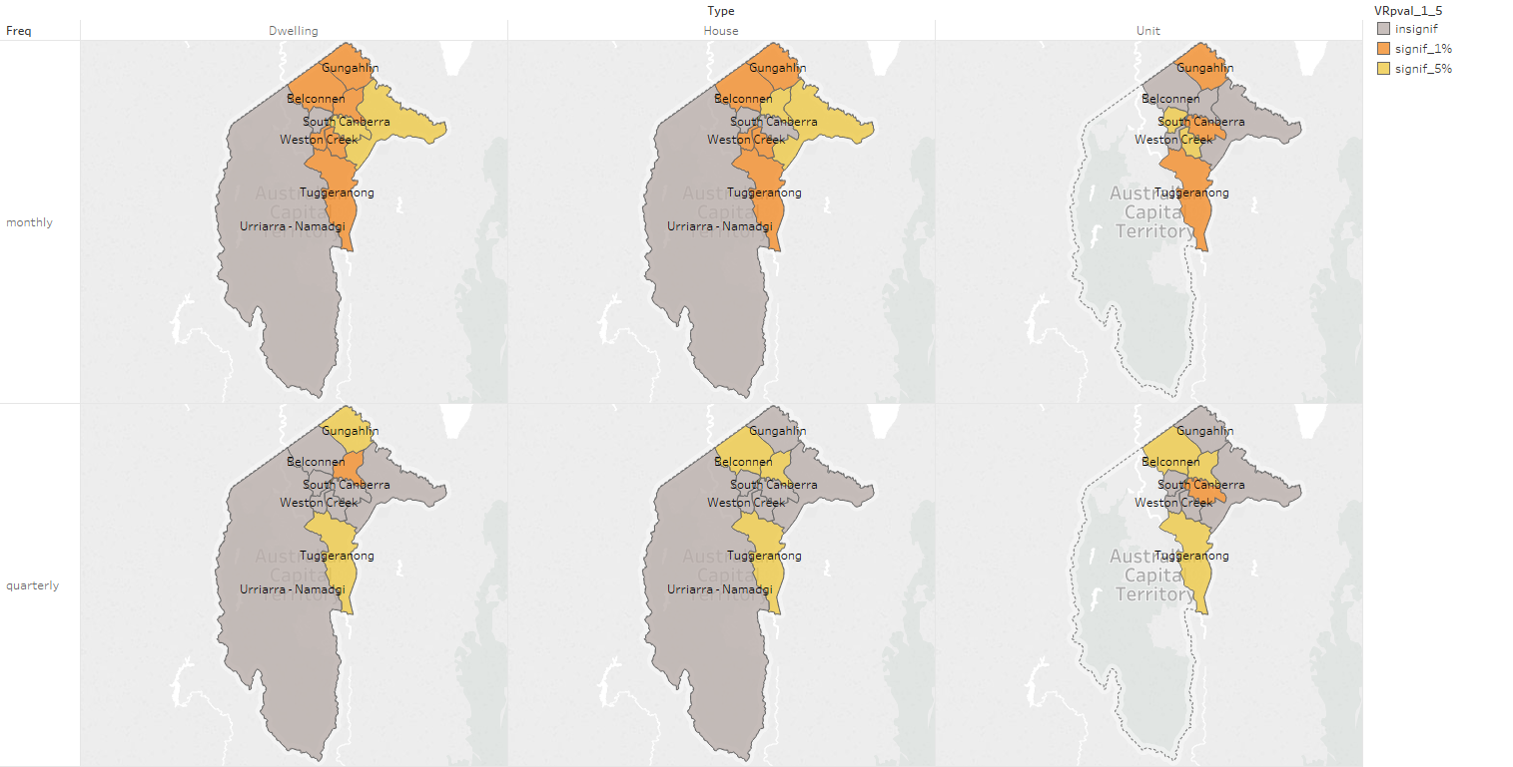
\includegraphics[width=\columnwidth]{Figures/maps_c_act.png}
 \caption{Persistence in Capital Returns at SA3 geographic level - Australian Capital Territory}
 \label{fig:maps_c_act}
\end{sidewaysfigure}

\begin{sidewaysfigure}[!htbp]
    \centering
     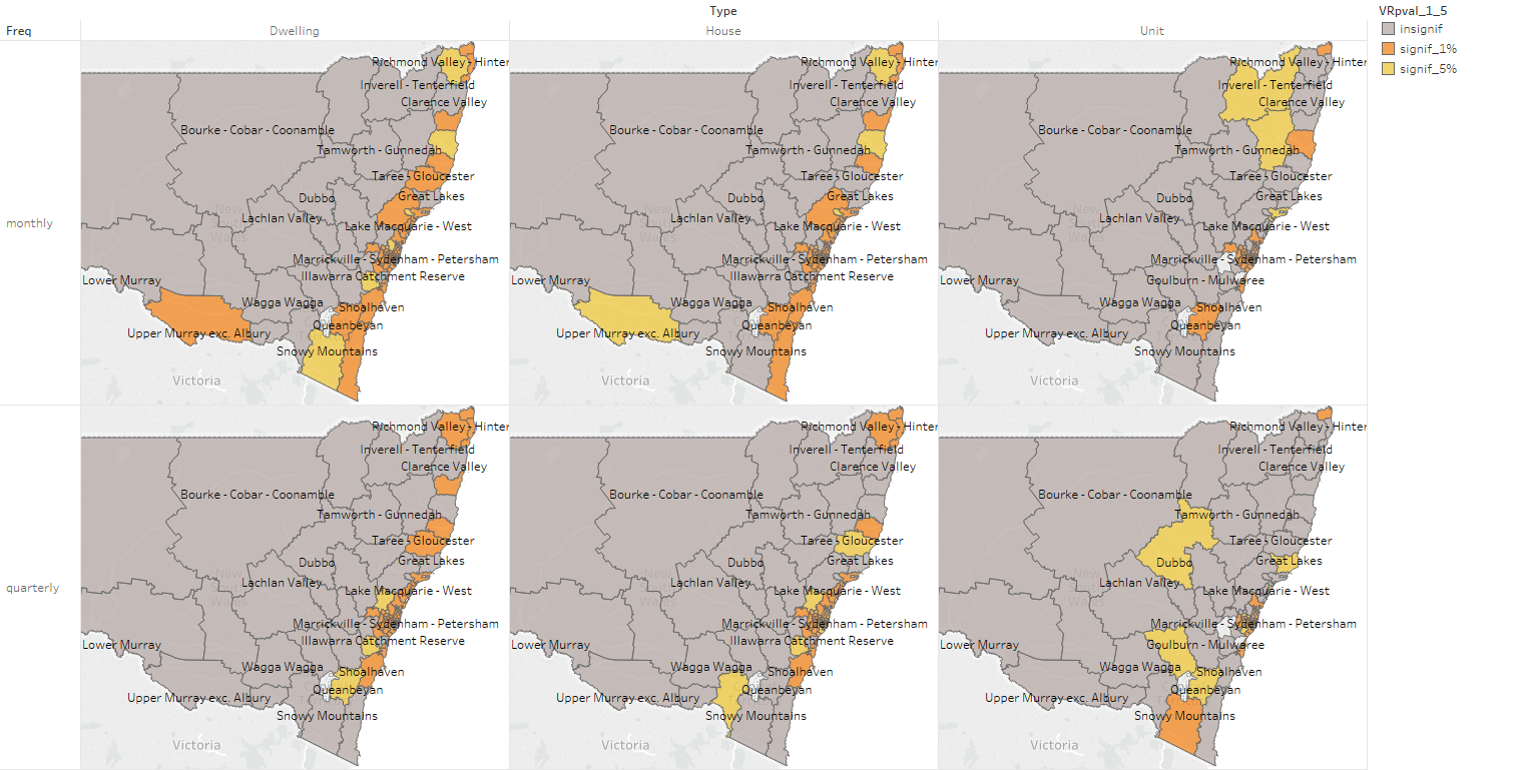
\includegraphics[width=\columnwidth]{Figures/maps_c_nsw.png}
 \caption{Persistence in Capital Returns at SA3 geographic level - New South Wales}
 \label{fig:maps_c_nsw}
\end{sidewaysfigure}


\begin{sidewaysfigure}[!htbp]
    \centering
     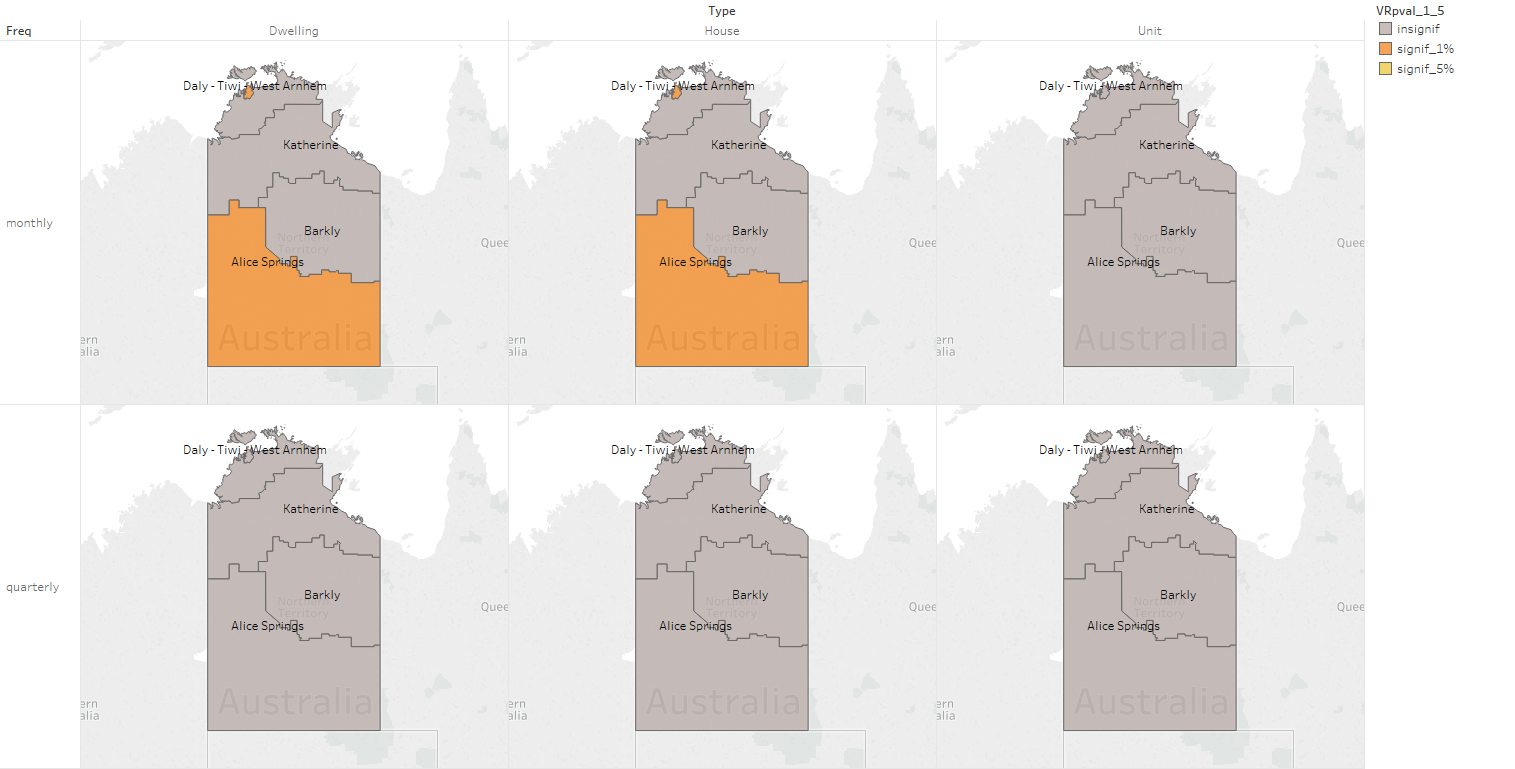
\includegraphics[width=\columnwidth]{Figures/maps_c_nt.png}
 \caption{Persistence in Capital Returns at SA3 geographic level - Northern Territory}
 \label{fig:maps_c_nt}
\end{sidewaysfigure}

\begin{sidewaysfigure}[!htbp]
    \centering
     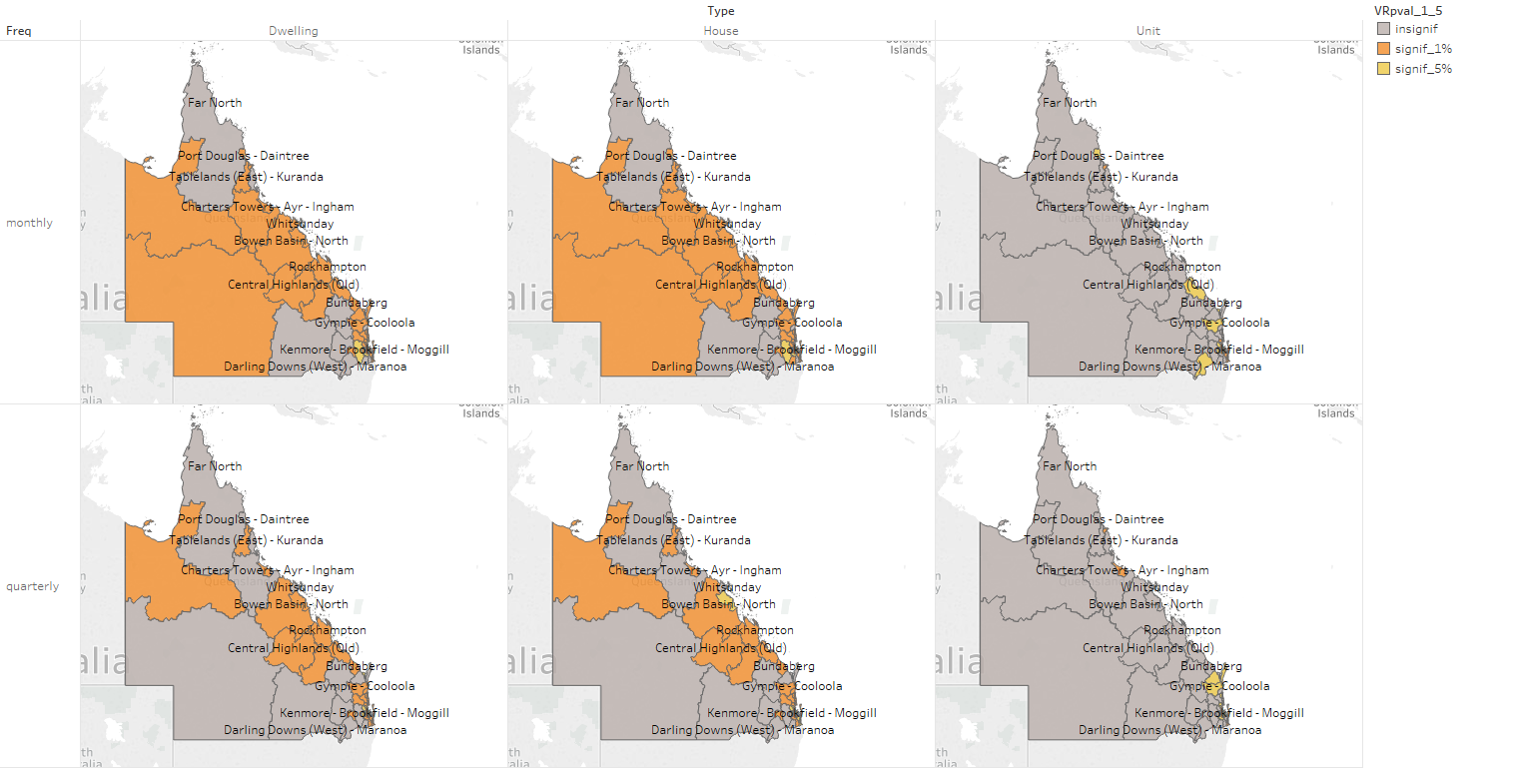
\includegraphics[width=\columnwidth]{Figures/maps_c_qld.png}
 \caption{Persistence in Capital Returns at SA3 geographic level - Queensland}
 \label{fig:maps_c_qld}
\end{sidewaysfigure}

\begin{sidewaysfigure}[!htbp]
    \centering
     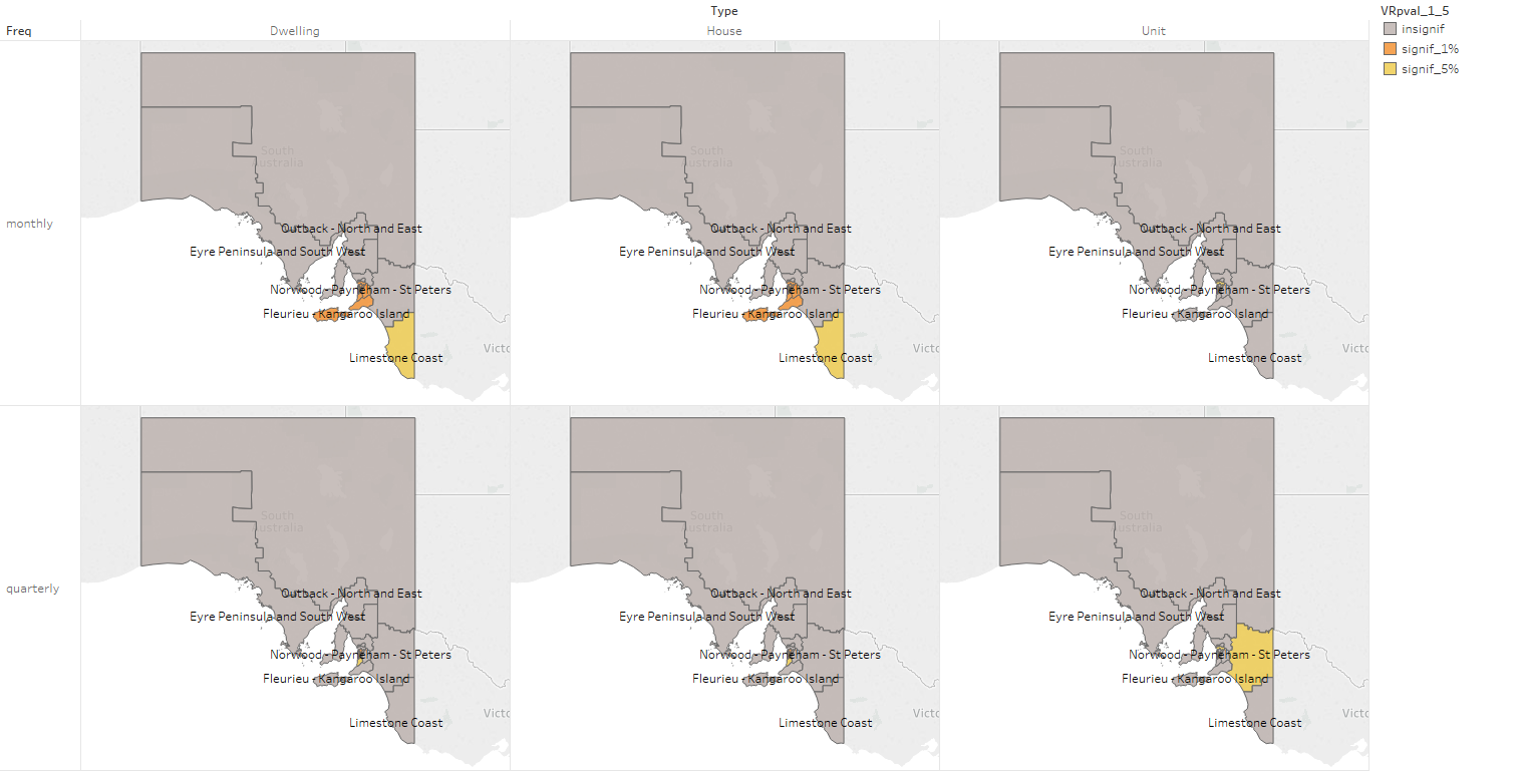
\includegraphics[width=\columnwidth]{Figures/maps_c_sa.png}
 \caption{Persistence in Capital Returns at SA3 geographic level - South Australia}
 \label{fig:maps_c_sa}
\end{sidewaysfigure}

\begin{sidewaysfigure}[!htbp]
    \centering
     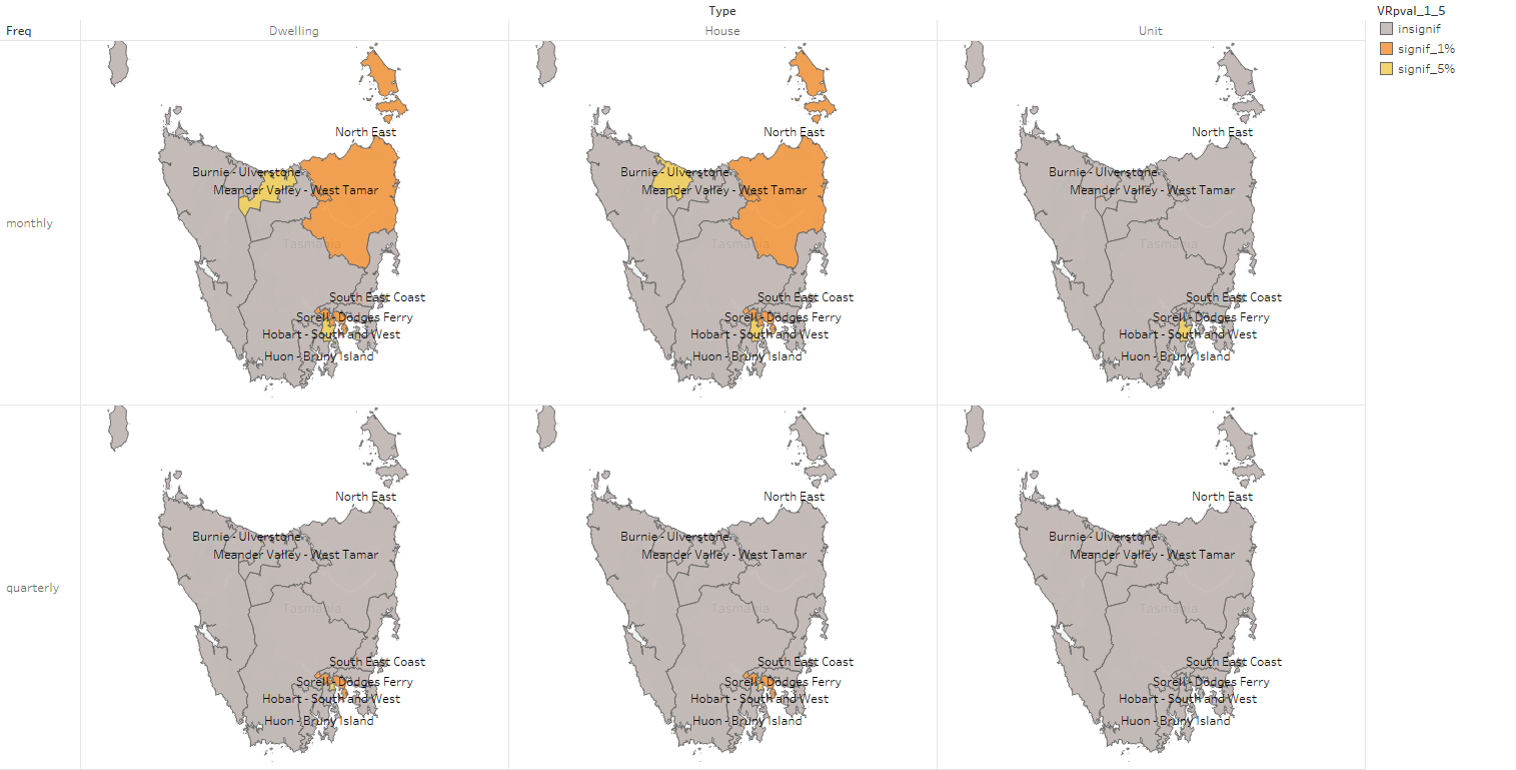
\includegraphics[width=\columnwidth]{Figures/maps_c_tas.png}
 \caption{Persistence in Capital Returns at SA3 geographic level - Tasmania}
 \label{fig:maps_c_tas}
\end{sidewaysfigure}

\begin{sidewaysfigure}[!htbp]
    \centering
     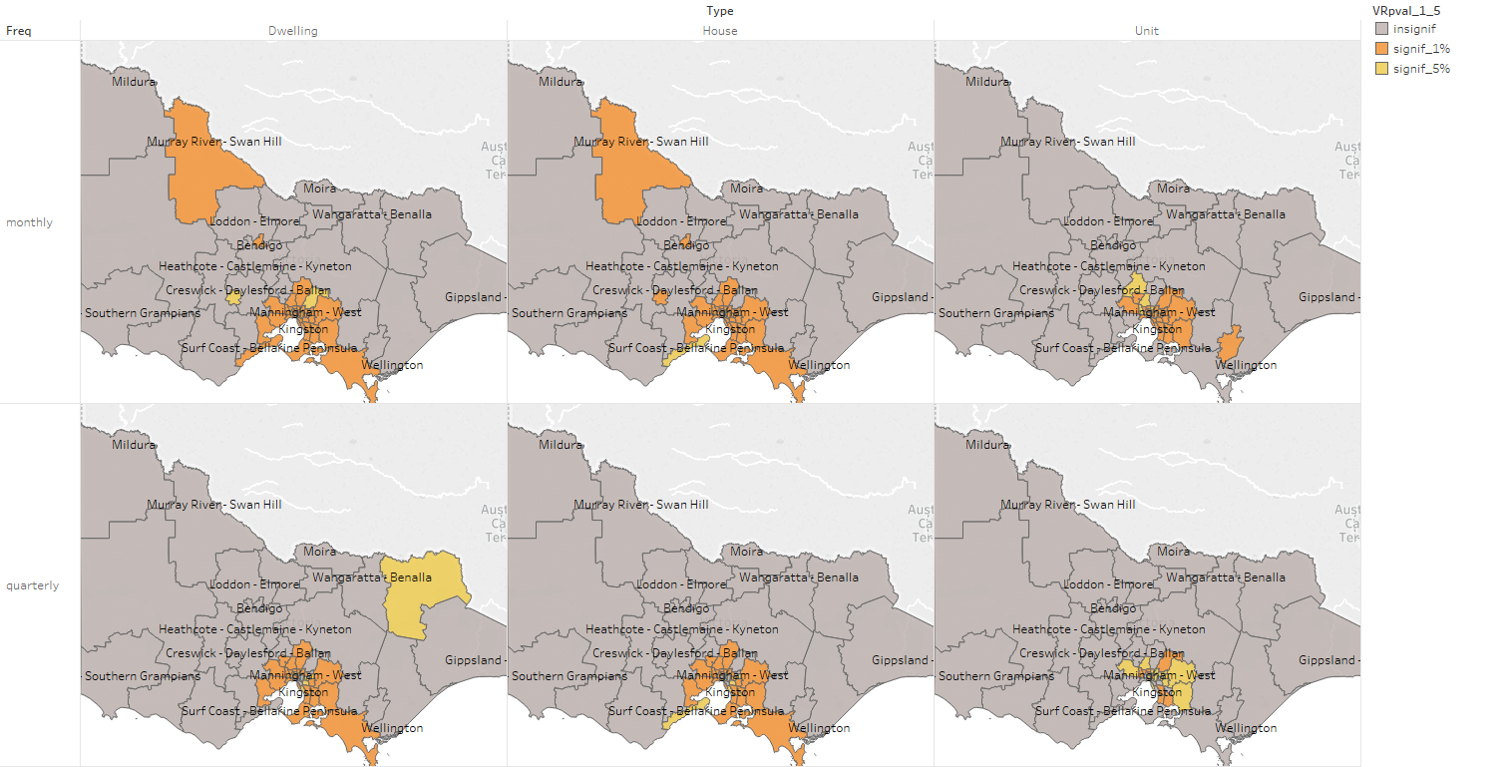
\includegraphics[width=\columnwidth]{Figures/maps_c_vic.png}
 \caption{Persistence in Capital Returns at SA3 geographic level - Victoria}
 \label{fig:maps_c_vic}
\end{sidewaysfigure}

\begin{sidewaysfigure}[!htbp]
    \centering
     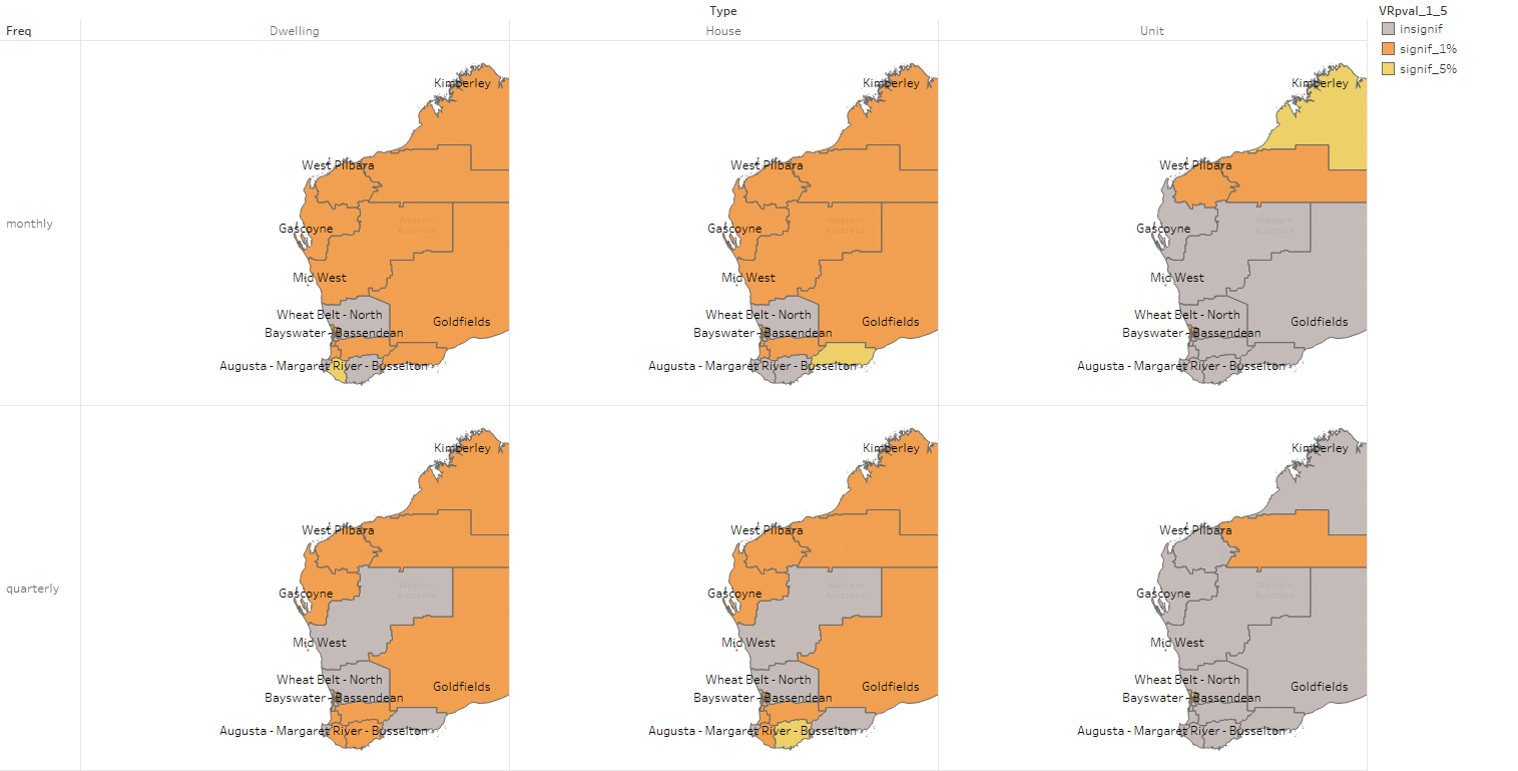
\includegraphics[width=\columnwidth]{Figures/maps_c_wa.png}
 \caption{Persistence in Capital Returns at SA3 geographic level - Western Australia}
 \label{fig:maps_c_wa}
\end{sidewaysfigure}

\begin{sidewaysfigure}[!htbp]
    \centering
     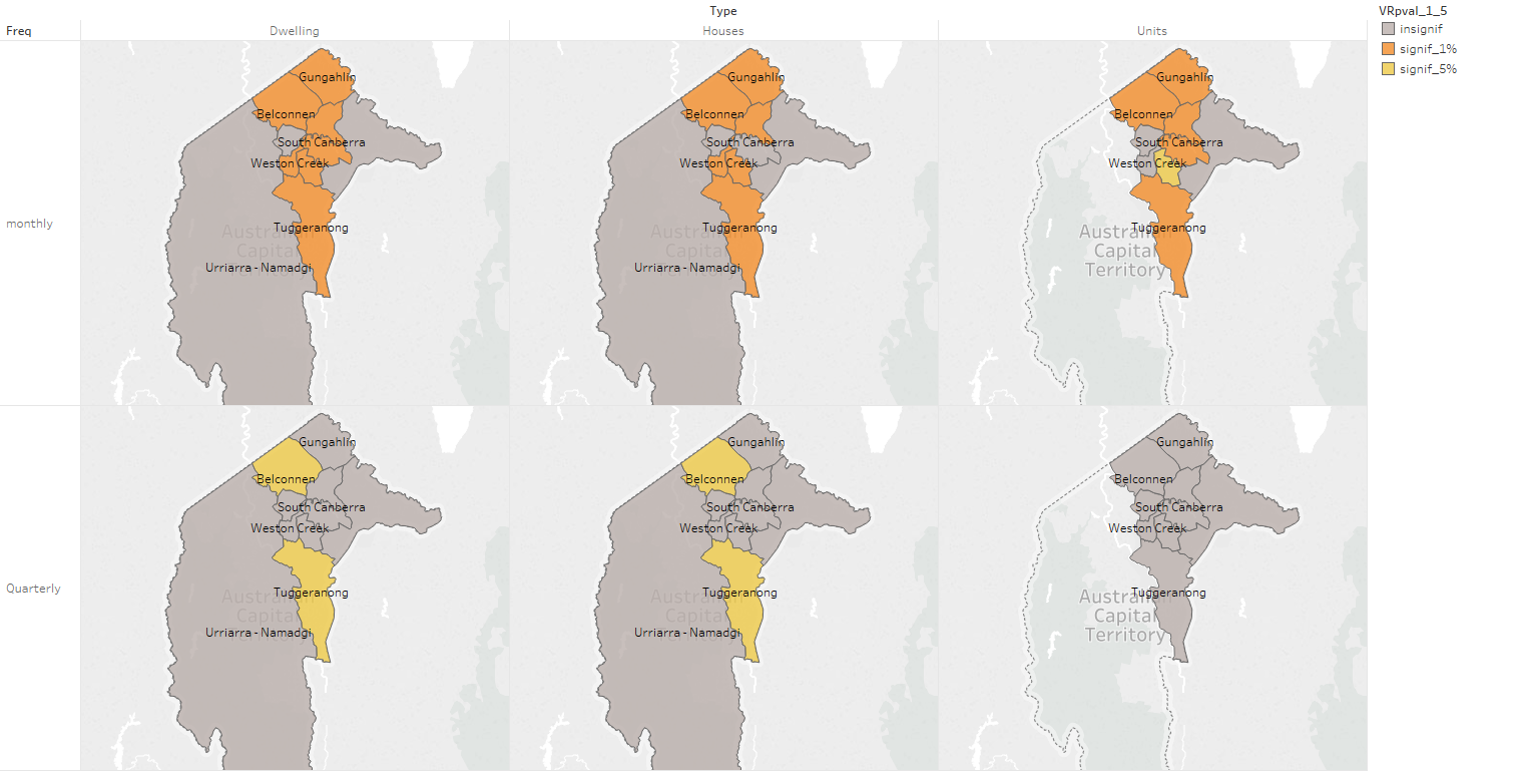
\includegraphics[width=\columnwidth]{Figures/maps_r_act.png}
 \caption{Persistence in Rental Returns at SA3 geographic level - Australian Capital Territory}
 \label{fig:maps_r_act}
\end{sidewaysfigure}


\begin{sidewaysfigure}[!htbp]
    \centering
     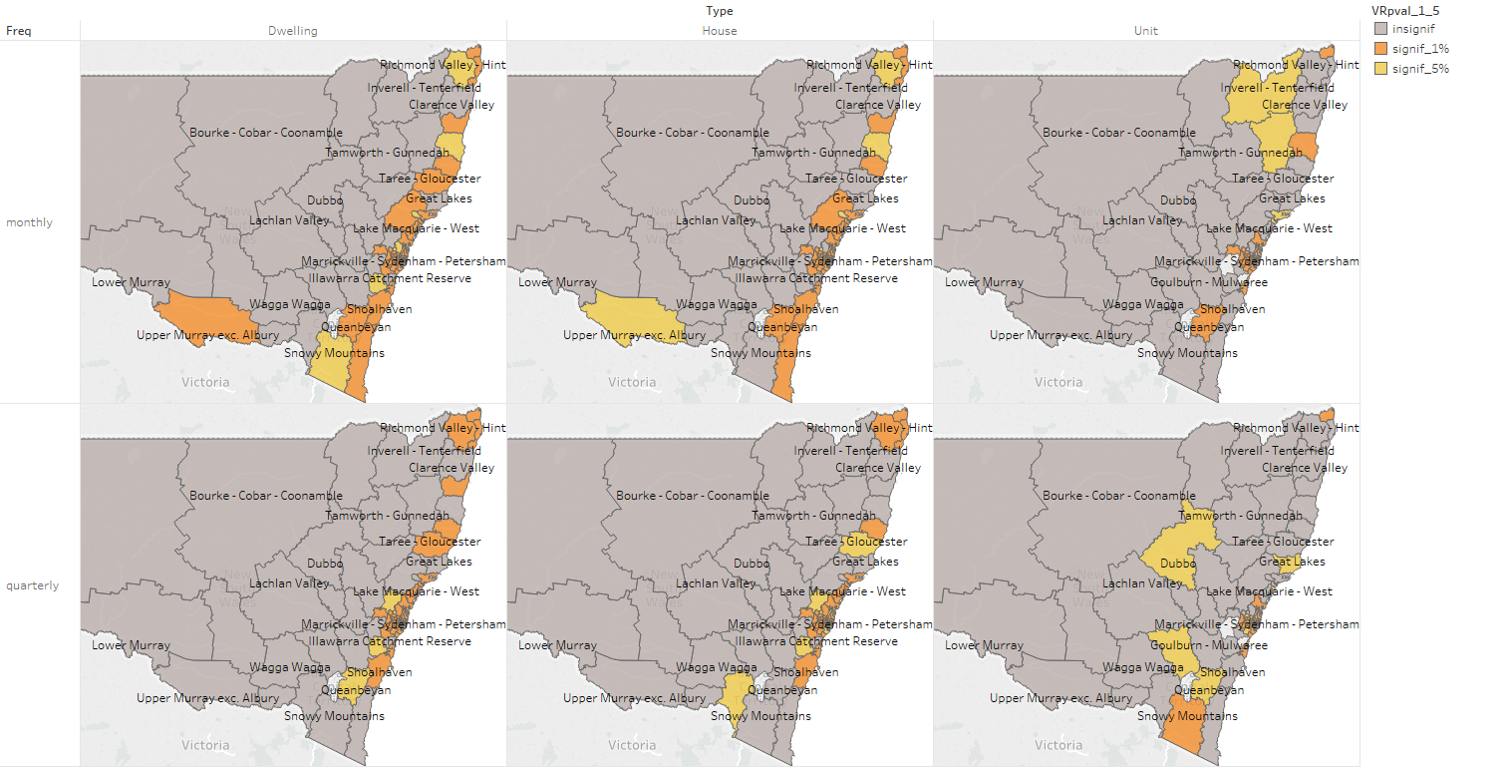
\includegraphics[width=\columnwidth]{Figures/maps_r_nsw.png}
 \caption{Persistence in Rental Returns at SA3 geographic level - New South Wales}
 \label{fig:maps_r_nsw}
\end{sidewaysfigure}

\begin{sidewaysfigure}[!htbp]
    \centering
     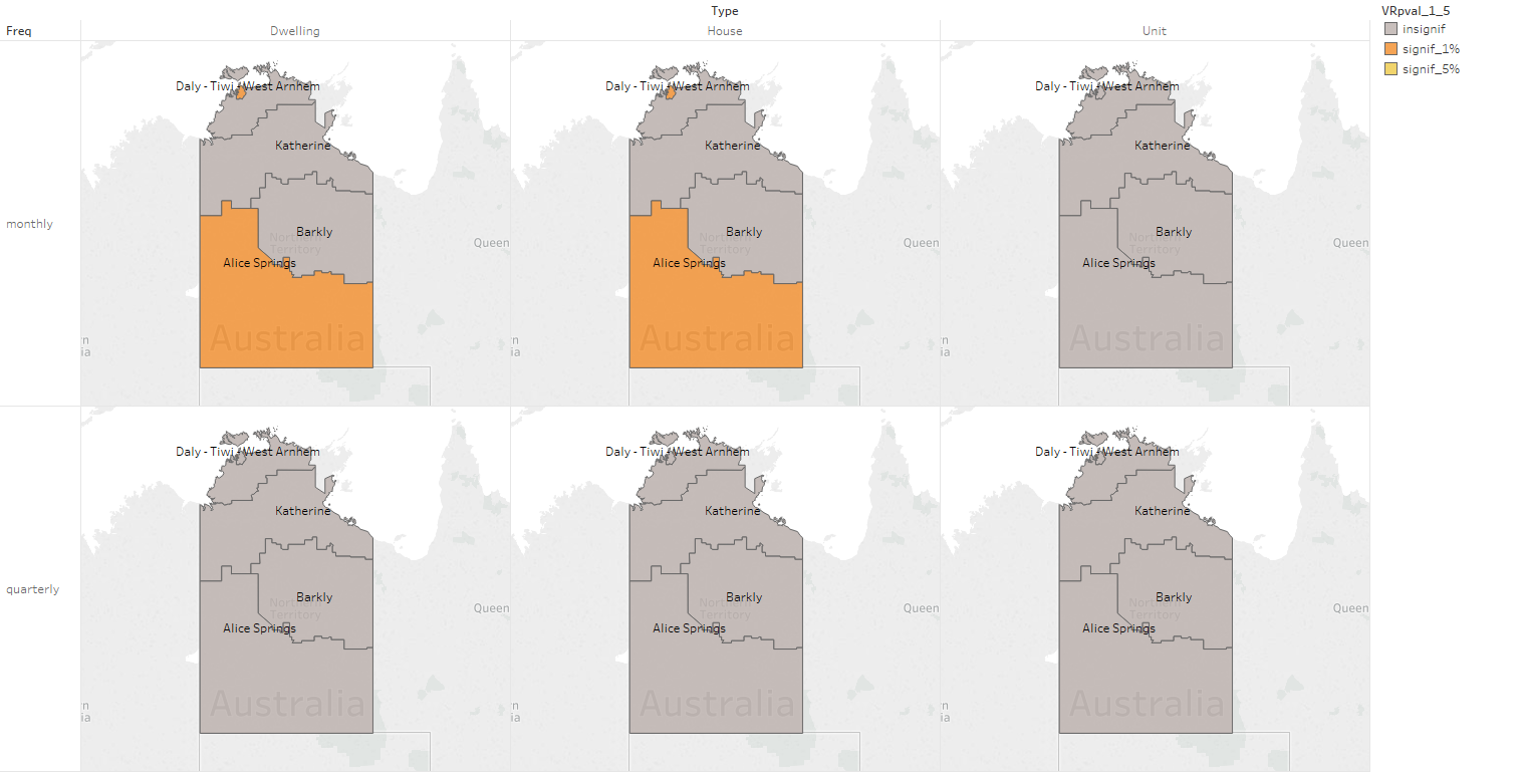
\includegraphics[width=\columnwidth]{Figures/maps_r_nt.png}
 \caption{Persistence in Rental Returns at SA3 geographic level - Northern Territory}
 \label{fig:maps_r_nt}
\end{sidewaysfigure}

\begin{sidewaysfigure}[!htbp]
    \centering
     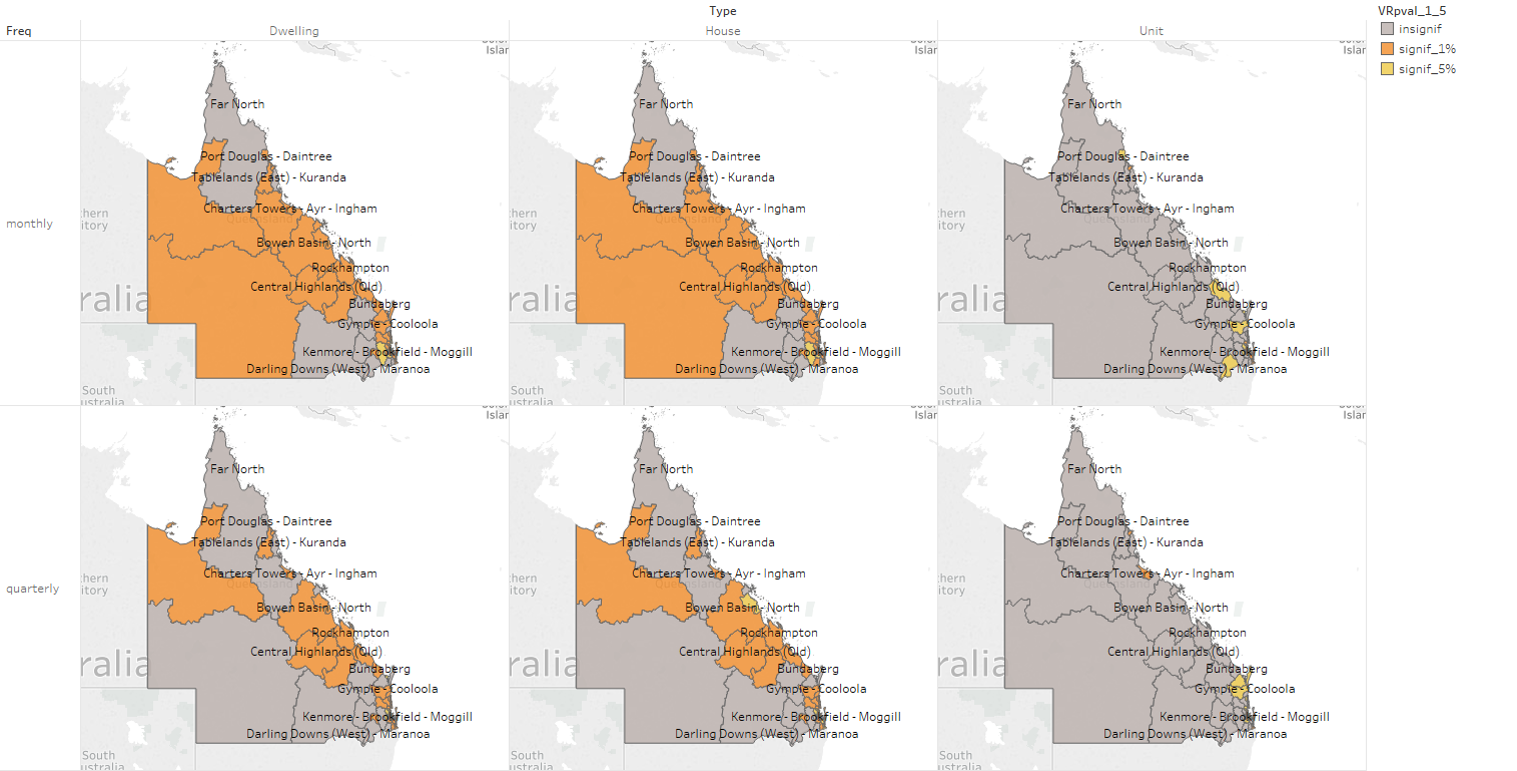
\includegraphics[width=\columnwidth]{Figures/maps_r_qld.png}
 \caption{Persistence in Rental Returns at SA3 geographic level - Queensland}
 \label{fig:maps_r_qld}
\end{sidewaysfigure}

\begin{sidewaysfigure}[!htbp]
    \centering
     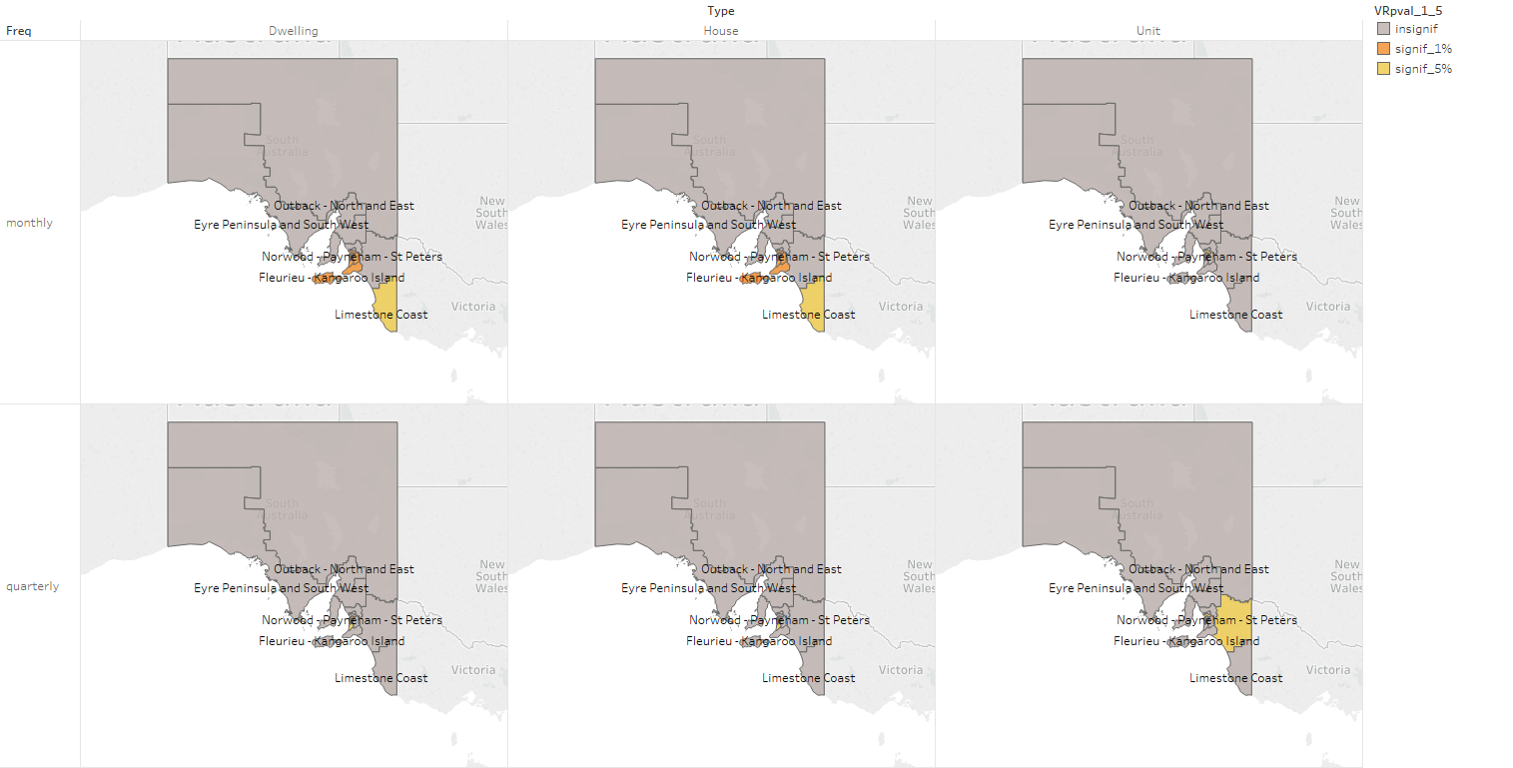
\includegraphics[width=\columnwidth]{Figures/maps_r_sa.png}
 \caption{Persistence in Rental Returns at SA3 geographic level - South Australia}
 \label{fig:maps_r_sa}
\end{sidewaysfigure}


\begin{sidewaysfigure}[!htbp]
    \centering
     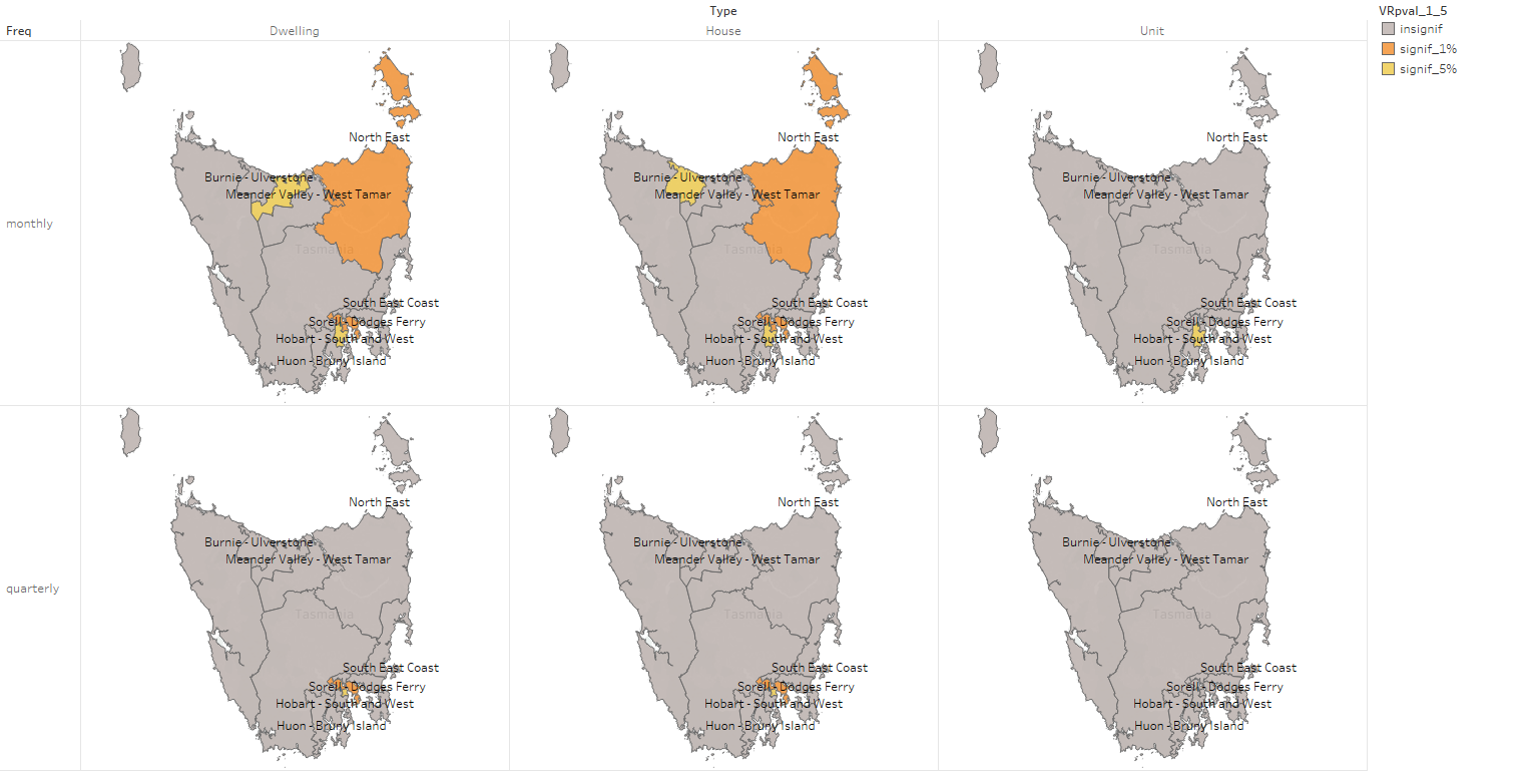
\includegraphics[width=\columnwidth]{Figures/maps_r_tas.png}
 \caption{Persistence in Rental Returns at SA3 geographic level - Tasmania}
 \label{fig:maps_r_tas}
\end{sidewaysfigure}

\begin{sidewaysfigure}[!htbp]
    \centering
     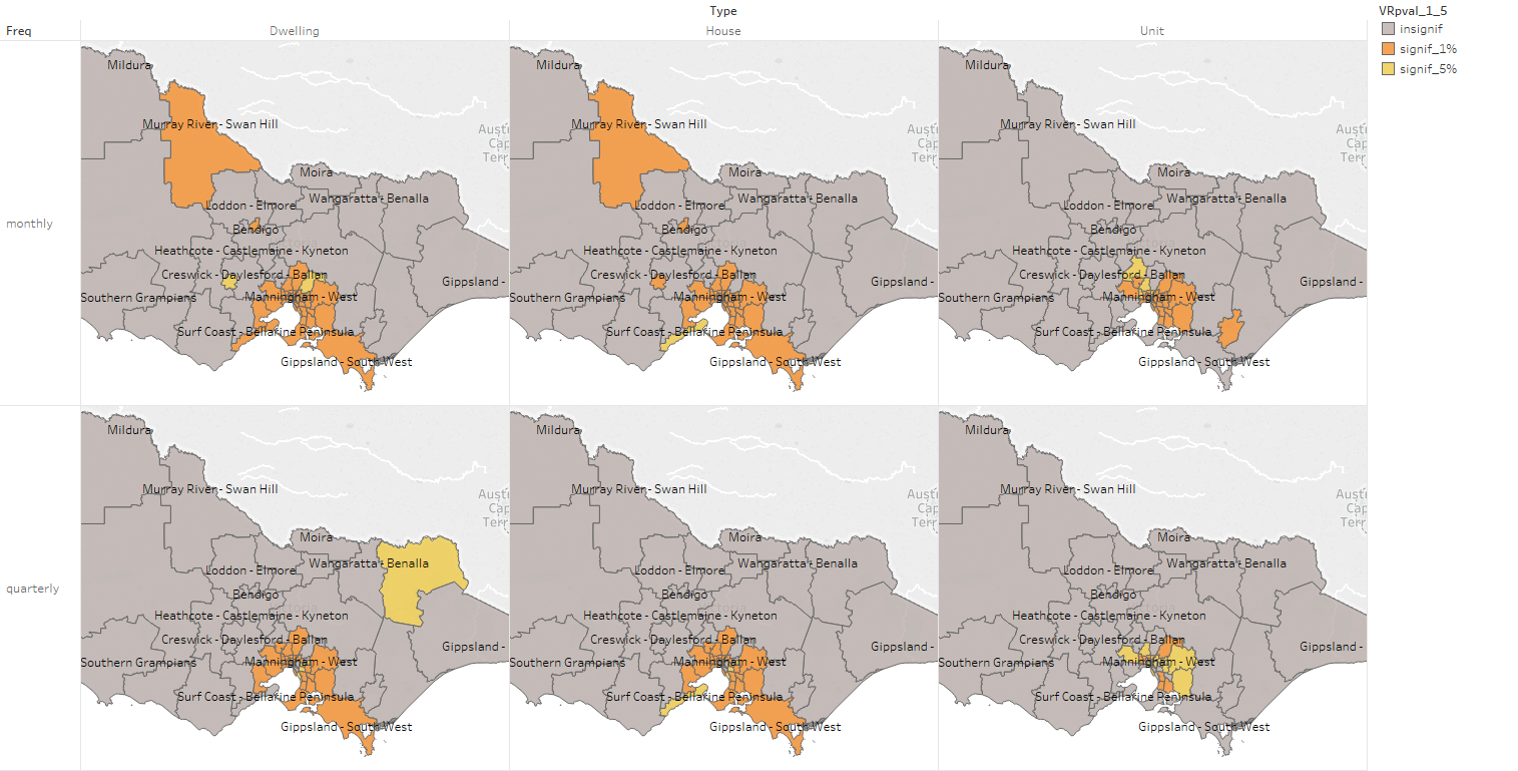
\includegraphics[width=\columnwidth]{Figures/maps_r_vic.png}
 \caption{Persistence in Rental Returns at SA3 geographic level - Victoria}
 \label{fig:maps_r_vic}
\end{sidewaysfigure}

\begin{sidewaysfigure}[!htbp]
    \centering
     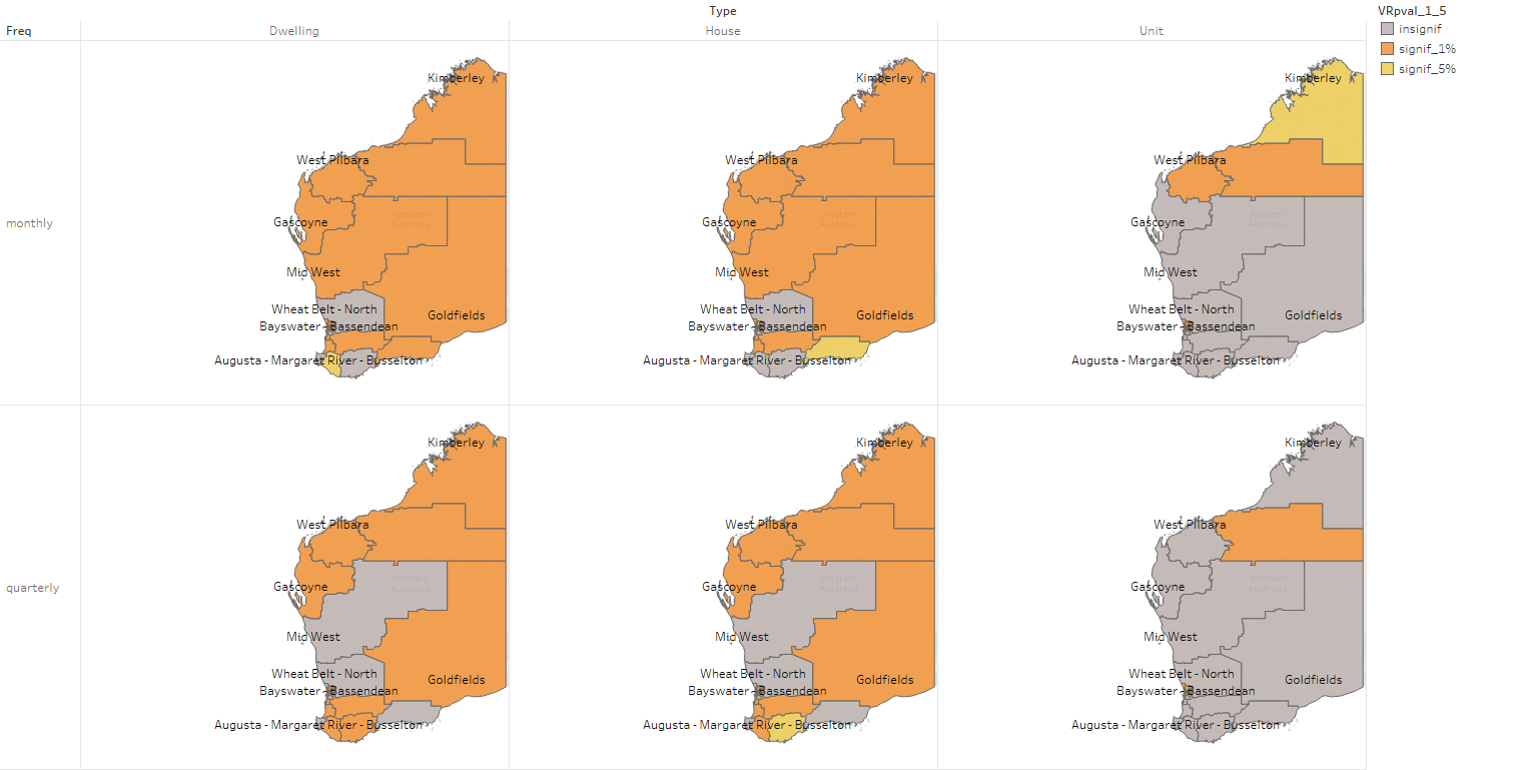
\includegraphics[width=\columnwidth]{Figures/maps_r_wa.png}
 \caption{Persistence in Rental Returns at SA3 geographic level - Western Australia}
 \label{fig:maps_r_wa}
\end{sidewaysfigure}

\restoregeometry
\end{comment}


\end{document}

